\documentclass[letterpaper,12pt,oneside,final]{book}
%%
%%  Template de mémoire de maîtrise ou thèse de doctorat.
%%  Normalement, il n'est pas nécessaire de modifier ce document
%%  sauf pour changer les noms des fichiers à inclure.
%%
%%  Version: 2014-10-28
%%
%%  Accepte les caractères accentués dans le document (UTF-8).
\usepackage[utf8]{inputenc}
%%
%% Support pour l'anglais et le français (français par défaut).
%\usepackage[cyr]{aeguill}
\usepackage{lmodern}      % Police de caractères plus complète et généralement indistinguable visuellement de la police standard de LaTeX (Computer Modern).
\usepackage[T1]{fontenc}  % Bon encodage des caractères pour qu'Acrobat Reader reconnaisse les accents et les ligatures telles que ffi.
\usepackage[english,frenchb]{babel} % le langage par défaut est le dernier de la liste, c'est-à-dire français
%%
%% Charge le module d'affichage graphique.
\usepackage{graphicx}
\usepackage{epstopdf}  % Permet d'utiliser des .eps avec pdfLaTeX.
\usepackage[author={Andre Nguyen}]{pdfcomment}
\usepackage{svg}
%%
%% Recherche des images dans les répertoires.
\graphicspath{{./images/}{./dia/}{./gnuplot/}}
%%
%% Un float peut apparaître seulement après sa définition, jamais avant.
\usepackage{flafter,placeins}
%%
%% Utilisation de natbib pour les citations et la bibliographie.
\usepackage{natbib}
%%
%% Autres packages.
\usepackage{amsmath,amssymb,color,soulutf8,longtable,colortbl,setspace,ifthen,xspace,url,pdflscape,bm}
\usepackage{mathtools}
\usepackage[linesnumbered,lined,boxed,commentsnumbered,ruled,vlined,french]{algorithm2e}

\newlength{\commentWidth}
\setlength{\commentWidth}{7cm}
\newcommand{\atcp}[1]{\tcp*[r]{\makebox[\commentWidth]{#1\hfill}}}
\newenvironment{sbmatrix}[1]
 {\def\mysubscript{#1}\mathop\bgroup\begin{bmatrix}}
 {\end{bmatrix}\egroup_{\textstyle\mathstrut\mysubscript}}

\def\code#1{\texttt{#1}}
\newcommand{\vect}[1]{\mathbf{#1}}
\DeclareMathOperator{\atantwo}{atan2}
\usepackage[group-separator={,}]{siunitx}

\newcommand\incomplete{\color{red}Incomplete\color{black}}
%%
%% Support des acronymes.
\usepackage[nolist]{acronym}
\onehalfspacing                % Interligne 1.5.
%%
%% Définition d'un style de page avec seulement le numéro de page à
%% droite. On s'assure aussi que le style de page par défaut soit
%% d'afficher le numéro de page en haut à droite.
\usepackage{fancyhdr}
\fancypagestyle{pagenumber}{\fancyhf{}\fancyhead[R]{\thepage}}
\renewcommand\headrulewidth{0pt}
\makeatletter
\let\ps@plain=\ps@pagenumber
\makeatother
%%
%% Module qui permet la création des bookmarks dans un fichier PDF.
%\usepackage[dvipdfm]{hyperref}
\usepackage{hyperref}
\usepackage{caption}  % Hyperlien vers la figure plutôt que son titre.
\makeatletter
\providecommand*{\toclevel@compteur}{0}
\makeatother
%%
%% Définitions spécifiques au format de rédaction de Poly.
\usepackage{MemoireThese}
%%
%% Définitions spécifiques à l'étudiant.
% !TEX root = Document.tex
% !TeX spellcheck = fr
%% -----------------------------------
%% ---> A MODIFIER PAR L'ETUDIANT <---
%% -----------------------------------
%%
%% Commandes qui affichent le titre du document, le nom de l'auteur, etc.
\newcommand\monTitre{Méthodes d'inspection automatique d'infrastructure par robot mobile}
\newcommand\monPrenom{Andre Phu-Van}
\newcommand\monNom{Nguyen}
\newcommand\monDepartement{Génie Électrique}
\newcommand\maDiscipline{génie électrique}
\newcommand\monDiplome{M}        % (M)aîtrise ou (D)octorat
\newcommand\anneeDepot{2017}
\newcommand\moisDepot{décembre}
\newcommand\monSexe{M}           % "M" ou "F"
\newcommand\PageGarde{O}         % "O" ou "N"
\newcommand\AnnexesPresentes{O}  % "O" ou "N". Indique si le document comprend des annexes.
\newcommand\mesMotsClef{Liste,de,mot-clés,séparés,par,des,virgules}
%%
%%  DEFINITION DU JURY
%%
%%  Pour la définition du jury, les macros suivantes sont definies:
%%  \PresidentJury, \DirecteurRecherche, \CoDirecteurRecherche, \MembreJury, \MembreExterneJury
%%
%%  Toutes les macros prennent 4 paramètres: Sexe (M/F), Prénom, Nom, Titres
\newcommand\monJury{\PresidentJury{M}{Richard}{Gourdeau}{Ph.~D.}\\
\DirecteurRecherche{M}{Jérôme}{Le ny}{Ph.~D.}\\
\CoDirecteurRecherche{M}{David}{SAUSSIÉ}{Ph.~D.}\\
\MembreJury{M}{Liam}{Paull}{Ph.~D.}}

\ifthenelse{\equal{\monDiplome}{M}}{
\newcommand\monSujet{Mémoire de maîtrise}
\newcommand\monDipl{Maîtrise ès sciences appliquées}
}{
\newcommand\monSujet{Thèse de doctorat}
\newcommand\monDipl{Philosophi\ae{} Doctor}
}
%%
%% Informations qui sont stockées dans un fichier PDF.
\hypersetup{
  pdftitle={\monTitre},
  pdfsubject={\monSujet},
  pdfauthor={\monPrenom{} \monNom},
  pdfkeywords={\mesMotsClef},
  bookmarksnumbered,
  pdfstartview={FitV},
  hidelinks,
  linktoc=all
}
%%
%% Il y a un document par chapitre du mémoire.
%%
\begin{document}
%%
%% Page de titre du mémoire.
\frontmatter
% Compte optionellement la page de garde dans la pagination.
\ifthenelse{\equal{\PageGarde}{O}}{\addtocounter{page}{1}}{}
\thispagestyle{empty}%
\begin{center}%
\vspace*{\stretch{1}}
UNIVERSITÉ DE MONTRÉAL\\
\vspace*{\stretch{1}}
\MakeUppercase{\monTitre}\\
\vspace*{\stretch{1}}
\MakeUppercase{\monPrenom~\monNom}\\
DÉPARTEMENT DE \MakeUppercase{\monDepartement}\\
ÉCOLE POLYTECHNIQUE DE MONTRÉAL\\
\vspace*{\stretch{1}}
\ifthenelse{\equal{\monDiplome}{M}}{MÉMOIRE PRÉSENTÉ}{THÈSE PRÉSENTÉE} EN VUE DE L'OBTENTION\\
DU DIPLÔME DE \MakeUppercase{\monDipl}\\
(\MakeUppercase{\maDiscipline})\\
\MakeUppercase{\moisDepot} \anneeDepot
\end{center}%
\vspace*{\stretch{1}}
\copyright~\monPrenom~\monNom, \anneeDepot.
%%
%% Identification des membres du jury.
%%
\newpage\thispagestyle{empty}%
\begin{center}%
\vspace*{\stretch{2}}
\ul{UNIVERSITÉ DE MONTRÉAL}\\
\vspace*{\stretch{1}}
\ul{ÉCOLE POLYTECHNIQUE DE MONTRÉAL}\\
\vspace*{\stretch{2}}
Ce\ifthenelse{\equal{\monDiplome}{M}}{~mémoire intitulé}{tte thèse intitulée}:\\
\vspace*{\stretch{1}}
\MakeUppercase{\monTitre}\\
\vspace*{\stretch{2}}
\end{center}%
\begin{flushleft}
présenté\ifthenelse{\equal{\monDiplome}{M}}{}{e}
par:~\ul{\mbox{\MakeUppercase{\monNom} \monPrenom}}\\
en vue de l'obtention du diplôme de:~\ul{\mbox{\monDipl}}\\
a été dûment accepté\ifthenelse{\equal{\monDiplome}{M}}{}{e} par le jury d'examen constitué de:\end{flushleft}
\vspace*{\stretch{2}}
\monJury
%%
\pagestyle{pagenumber}%
%% Dédicace
%%
%% La dédicace est un hommage que l'auteur souhaite
%% rendre à une ou plusieurs personnes de son choix.
%%
\chapter*{DÉDICACE}\thispagestyle{headings}
\addcontentsline{toc}{compteur}{DÉDICACE}
\begin{flushright}
  \itshape
  Je dédie ce travail à la mémoire de Dopey,\\
  ami, frère, chien,\\
  woof woof.
\end{flushright}
\setcounter{page}{3}
          % Dédicace du document.
% !TEX root = Document.tex
%!TeX spellcheck = fr
% Remerciements
%
%   Grâce aux remerciements, l'auteur attire l'attention du lecteur
% sur l'aide que certaines personnes lui ont apportée, sur leurs
% conseils ou sur toute autre forme de contribution lors de la
% réalisation de son mémoire. Le cas échéant, c'est dans cette section
% que le candidat doit témoigner sa reconnaissance à son directeur de
% recherche, aux organismes dispensateurs de subventions ou aux
% entreprises qui lui ont accordé des bourses ou des fonds de
% recherche.
\chapter*{REMERCIEMENTS}\thispagestyle{headings}
\addcontentsline{toc}{compteur}{REMERCIEMENTS}
%
%Je remercie mon chien Dopey pour le support émotionel à travers tout ce périple. Pour avoir toujours cru en moi et m'avoir supporté en temps de besoin.

Je tiens d'abord à remercier mes amis et collègues de laboratoire Alexandre Borowczyk, Dang Quang Nguyen, Duc Tien Nguyen et Gabriel Guilbert pour les fructueuses discussions théoriques et surtout pour avoir participé avec moi au DJI Challenge 2016. Ce fut la compétition d'ingénierie la plus difficile à laquelle j'ai participé durant mon cheminement académique et ce fut un honneur de l'avoir fait avec vous.

Je remercie aussi mes collègues Olivier Gougeon, Justin Cano, Jérémie Pilon, Catherine Massé et Juliette Tibayrenc pour les bons moments passés dans le Laboratoire de Robotique Mobile et des Systèmes Autonomes.

\newcommand{\RNum}[1]{\uppercase\expandafter{\romannumeral #1\relax}}

Je remercie Laurence Lebel, Alexandre Marceau-Gozsy, Simon Dufour, Mélanie Harvey, Simon Bourgault-Côté, Yoann Arpin, Marie Tardif-Drolet, Gabriel Brassard, Khaldoun El-Hajj, Marc Castanet, Alessandro Scola, Hubert Courteau-Godmaire, Félix Amyot et toutes les autres personnes que j'ai pu côtoyer lors de la construction de la voiture solaire Esteban \RNum{6}. Les deux années que j'ai passé dans l'équipe avec vous étaient essentielles à ma formation d'ingénieur et m'ont amenées à étendre mes connaissances bien au-delà des sujets de l'informatique.

Je remercie Antoine Mignon, Marc-André Ruel, David Thibodeau, Laurier Loiselle, Antonio Sanniravong, Constant Rietsch, Jean-Aleandre Barszcz, Quentin Gili, Alexandre St-Onge, David Binet et toutes les autres personnes qui on aidé de près ou de loin à la formation et l'opération de l'équipe du multirotor autonome Élikos. Je suis fier d'avoir bâti avec vous un projet d'envergure dont la pérenité est maintenant assurée par une fortre tradition d'excellence. Mes deux ans en tant que directeur du projet (et nos deux premières place à l'\emph{International Aerial Robotics Competition}) ont été un facteur décisif dans ma poursuite du sujet de la robotique aérienne aux cycles supérieurs.

%Je remercie aussi Maude Carrier, le temps que l'on a passé ensemble dans le cours de Traitement des Signaux et d'Images fût bien amusant.

Finalement j'aimerais remercier mes directeurs de recherche Jérôme Le Ny et David Saussié pour avoir accepté de superviser mes travaux de maîtrise et pour m'avoir aidé sans relâche à travers tout mon parcours de maîtrise.
     % Remerciements.
% !TEX root = Document.tex
% !TeX spellcheck = fr
% Résumé du mémoire.
%
%   Le résumé est un bref exposé du sujet traité, des objectifs visés,
% des hypothèses émises, des méthodes expérimentales utilisées et de
% l'analyse des résultats obtenus. On y présente également les
% principales conclusions de la recherche ainsi que ses applications
% éventuelles. En général, un résumé ne dépasse pas quatre pages.
%
%   Le résumé doit donner une idée exacte du contenu du mémoire ou de la thèse. Ce ne
% peut pas être une simple énumération des parties du document, car il
% doit faire ressortir l'originalité de la recherche, son aspect
% créatif et sa contribution au développement de la technologie ou à
% l'avancement des connaissances en génie et en sciences appliquées.
% Un résumé ne doit jamais comporter de références ou de figures.
\chapter*{RÉSUMÉ}\thispagestyle{headings}
\addcontentsline{toc}{compteur}{RÉSUMÉ}

La robotique est un domaine voué à la création de machines permettant d'aider
ou de remplacer les humains lors de tâches difficiles ou dangereuses. Plus souvent
utilisés dans le secteur manufacturier ou la recherche et sauvetage, les robots
trouvent maintenant leur place dans les secteurs de l'arpentage et l'inspection
d'infrastructure civile grâce à leur mobilité et leur capacité à effectuer des
tâches répétitives. Cependant, ces robots sont souvent encore opérés à distance
et ne possèdent que de l'autonomie partielle, étant toujours incapable de prendre
des décisions eux-mêmes.

Dans ce mémoire, nous tentons de répondre à ce problème en présentant deux
méthodes permettant de guider un robot autour d'une structure pour en faire
l'inspection. Premièrement, nous attaquons le problème d'inspection au sol de
structures fermées. Fonctionnant au moyen d'un robot terrestre équipé d'une
caméra de profondeur, notre méthode permet de cartographier la surface visible
d'une structure fermée. En particulier, nous proposons un système qui cherche
à effectuer l'inspection tout en minimisant la possibilité d'erreur sur le système
de localisation du robot. Deuxièmement, nous proposons un système spécifiquement
pour l'inspection d'éoliennes. Au moyen d'un véhicule aérien
non habité et de scanneurs lasers 2D, notre méthode permet à un quadricoptère de décoller
du sol et suivre la tour pour ensuite automatiquement parcourir la surface avant
des pales d'une éolienne.

Nos systèmes sont tous les deux implémentés et démontrés dans des environnements
de simulation. L'inspection terrestre est démontrée sur un vrai robot dans un
scénario d'inspection intérieur et nous présentons des résultats préliminaires
sur le déploiement de l'inspection aérienne.
      % Résumé du sujet en français.
% !TEX root = Document.tex
% !TeX spellcheck = en
% Abstract
%
%   Résumé de la recherche écrit en anglais sans être
% une traduction mot à mot du résumé écrit en français.

\chapter*{ABSTRACT}\thispagestyle{headings}
\addcontentsline{toc}{compteur}{ABSTRACT}
%
\begin{otherlanguage}{english}

Robotics is a branch of engineering dealing with the creation of machines capable
of helping or even replacing humans in tasks which can be dull, dirty or dangerous.
Most commonly used in the fields of manufacturing and search and rescue, in recent
years robotics has found its place in surveying and infrastructure inspection
thanks to their increased mobility and their ability to tackle repetitive tasks.
However, today's robots are still often remote controlled with only
partial autonomy and still aren't capable of decision making and navigation.

In this thesis, we address this problem by presenting two methods allowing a robot
to navigate around a structure to inspect its surface. First, we tackle
the problem of ground based inspections of the visible part of a bounded closed
structure. Using an unmanned ground vehicle equipped with a depth sensor, our
method allows us to map the entire surface of the structure. Our specific
contribution here, is a system capable of performing the inspection while also
minimizing errors on the robot's localization system. Also known as "active slam",
we perform path planning for exploration while also performing SLAM. Second, we
propose a system specifically tailored to the inspection of wind turbines. Using
an unmanned aerial vehicle equipped with 2D laser scanners, our method allows
a quadcopter to take off, climb up the tower and inspect the front facing
surface of the turbine's blades.

Both of our systems are implemented and shown to work within simulation environments.
Our ground based inspection is also demonstrated in real indoor experiments where
we show how to deal with noise not accounted for in simulation.
Finally, we also show preliminary results on the deployment of our wind turbine inspection
system.

\end{otherlanguage}
          % Résumé du sujet en anglais.

{\setlength{\parskip}{0pt}
%%
%% Table des matières.
\renewcommand\contentsname{TABLE DES MATIÈRES}
\tableofcontents
%%
%% Liste des tableaux.
\renewcommand\listtablename{LISTE DES TABLEAUX}
\listoftables
%%
%% Table des figures.
\renewcommand\listfigurename{LISTE DES FIGURES}
\listoffigures
%%
%% Liste des annexes au besoin.
}

% !TEX root = Document.tex
% Liste des sigles et abbréviations
\newcommand\abbrevname{LISTE DES SIGLES ET ABRÉVIATIONS}
\chapter*{\abbrevname}
\addcontentsline{toc}{compteur}{\abbrevname}
\pagestyle{pagenumber}
%
\begin{acronym}
  \acro{SLAM}{Simultaneous Localization And Mapping}
  \acro{UAV}{Unmanned Aerial Vehicle}
  \acro{UGV}{Unmanned Ground Vehicle}
\end{acronym}
%
\begin{longtable}{lp{3in}p{3in}}
          & English & Français\\
\hline          
GIS       & Geographical Information System & Système d'Information Géographique\\
GPS       & Global Positioning System & Système de Positionnement Global\\
IMU       & Inertial Measurement Unit & Centrale Inertielle\\
SLAM      & Simultaneous Localization And Mapping & Locatisation et Cartographie Simultanée\\
UAV       & Unmanned Aerial Vehicle & Véhicule Aérien Non-Habité\\
UGV       & Unmanned Ground Vehicle & Véhicule Terrestre Non-Habité\\
\end{longtable}
       % Liste des sigles et abréviations.
% !TEX root = Document.tex
\chapter*{Liste des publications}

\begin{longtable}{lp{5in}}
  [Journal]     & A. Borowczyk, D.-T. Nguyen, \textbf{A. Phu-Van Nguyen}, D. Q. Nguyen, D. Saussié and J. Le Ny, \textit{Autonomous Landing of a Quadcopter on a High-Speed Ground Vehicle}. AIAA Journal of Guidance, Control and Dynamics, In Press, 2017.\\

  [Conférence]  & A. Borowczyk, D.-T. Nguyen, \textbf{A. Phu-Van Nguyen}, D. Q. Nguyen, D. Saussié and J. Le Ny, \textit{Autonomous Landing of a Multirotor Micro Air Vehicle on a High Velocity Ground Vehicle}. Proceedings of the IFAC World Congress, Toulouse, France, July 2017.\\

  [Journal]      & M. S. Ramanagopal, \textbf{A. Phu-Van Nguyen} and J. Le Ny, A Motion Planning Strategy for the Active Vision-Based Mapping of Ground-Level Structures. Accepted by Transactions on Automation Science and Engineering, November 2017.
\end{longtable}

Le travail des deux premières publications à propos de l'atterrissage d'un quadricoptère sur une voiture en mouvement a été réalisé dans le cadre de la participation du \textit{Mobile Robotics and Autonomous Systems Laboratory} au DJI Challenge lors des session d'hiver et d'été 2016. N'étant pas directement liées au présent mémoire, elles sont mentionnées ici car plusieurs des méthodes de contrôle de véhicule aérien et de traitement d'images ont été apprises lors de notre participation à cette compétition.

La dernière publication intitulée \textit{A Motion Planning Strategy for the Active Vision-Based Mapping of Ground-Level Structures} a été initialement soumise en février 2016 par M. S. Ramanagopal et J. Le Ny au journal \textit{Transactions on Automation Science and Engineering} (T-ASE). Lors du retour de l'évaluation par les pairs, il a été demandé entres autres d'ajouter un volet expérimental à l'article afin de prouver la validité des algorithmes développés dans l'article. C'est à ce moment, lors de la session d'automne 2016 et au début de la session d'hiver 2017 que je me suis ajouté au projet pour faire l'implémentation sur un robot physique. Au moment de l'écriture du présent mémoire, l'article a été accepté pour publication dans une édition future du journal T-ASE. Nous présentons le travail réalisé dans le cadre de ce projet au Chapitre \ref{sec:ugv}.
       % Liste des sigles et abréviations.
\ifthenelse{\equal{\AnnexesPresentes}{O}}{\listofappendices}{}
\mainmatter
% !TEX root = Document.tex
%   Dans l'introduction, on présente le problème étudié et les buts
% poursuivis. L'introduction permet de faire connaître le cadre de la
% recherche et d'en préciser le domaine d'application. Elle fournit
% les précisions nécessaires en ce qui concerne le contexte de
% réalisation de la recherche, l'approche envisagée, l'évolution de
% la réalisation. En fait, l'introduction présente au lecteur ce
% qu'il doit savoir pour comprendre la recherche et en connaître la
% portée.
\Chapter{INTRODUCTION}\label{sec:Introduction}  % 10-12 lignes pour introduire le sujet.
Le domaine de la robotique s'applique à ce qui est communément appelé les trois \emph{D} de l'industrie \emph{Dull}, \emph{Dirty} et \emph{Dangerous}, c'est-à-dire les tâches ennuyantes, sales et dangereuses. L'inspection d'infrastructures civiles rentre dans la première et la dernière de celles-ci. Ennuyante car elle implique la cueillette répétitive de données et dangereuse car elle implique parfois l'obligation de grimper dans des structures hors de portée ou difficiles à atteindre.

En général, le but de ces inspections est multiple: outre la recherche de défauts dans l'infrastructure, elles peuvent aussi servir à suivre de près l'évolution d'un chantier de construction, faire de l'arpentage ou planifier de futurs projets de développement. L'intérêt de faire exécuter l'inspection par un robot autonome est d'une part d'accélérer la collecte de données par un robot plus mobile qu'un humain, et d'autre part de réduire les coûts liés à la collecte d'informations.

%\section{Problématique considérée}

%Dans ce projet nous distinguons deux types d'inspections: les inspections de structures au sol effectuées par un robot terrestre non-habité (UGV) et les inspections en hauteur effectuées par un robot aérien non-habité (UAV). Les deux cas comportent des similarités notamment par leurs besoin de systèmes de positionnement et de systèmes de planification de trajectoire.

\section{Objectif de recherche}

L'objectif principal de la recherche est de développer des méthodes d'inspection d'infrastructures adaptées aux robots terrestres non-habités (UGV) ainsi qu'aux robots aériens non-habités (UAV). La définition d'inspection peut varier d'un domaine à l'autre mais elle peut se résumer au déplacement d'un capteur quelconque pour recueillir de l'information sur l'entièreté d'un certain espace. Dans notre cas, nous traitons spécifiquement des scénarios où le capteur est une caméra ou une caméra de profondeur devant être déplacée pour capter la surface d'une structure et en reconstruire en modèle 3D.

Alors que la navigation du robot se fait entièrement de façon autonome, il est attendu qu'un opérateur intervienne seulement lors de la phase d'analyse des données et dans le cas d'un UAV qu'il intervienne dans la prise de photos.

\subsection{Inspections au sol}
Dans un premier lieu, nous nous attardons au problème de la création de cartes 3D précises de structures au sol. Ces cartes peuvent être utilisées pour une variété d'applications telles que la réalité virtuelle \citep{googlevr2017}, la navivation de véhicules autonomes \citep{deepmap2017} et la surveillance du progrès d'un chantier de construction \citep{Omar2018}. Cette dernière application, étant bien établie en industrie, se fait habituellement par l'une des trois méthodes suivantes: la photogrammétrie ou vidéogrammétrie \citep{BRILAKIS2011884}, les scanner lasers \citep{Turkan2012} ou même des caméras installées sur des véhicules aériens non-habités \citep{lin2015framework}. Chacune d'entres elles demande qu'un opérateur humain parcourt le chantier en cherchant les meilleurs points de vues avec les capteurs appropriés en main pour la collecte de données. En particulier, dû à la relative courte portée de capteurs d'images de profondeur, elles demandent aux opérateurs de parcourir une plus grande distance et plus de prises de vue.

C'est dans ce contexte que nous posons notre objectif de recherche qui est de guider un UGV pour faire l'inspection de la partie visible d'une structure au sol, au moyen d'un capteur de profondeur, sans aucune information \textit{a priori}. Pour commencer, nous nous basons sur des algorithmes de navigation et de localisation existants tels que les champs de potentiel, le Simultaneous Localization and Mapping (SLAM) visuel et la fusion d'odométrie de roues avec une centrale inertielle (IMU) pour effectuer le contrôle du véhicule. L'objectif est d'avoir une méthode de génération de trajectoires en temps réel qui, dans un premier temps, garanti la couverture entière de la surface de l'édifice, et dans un deuxième temps assure la précision du système de SLAM. Cet objectif secondaire complémente l'objectif primaire car la précision de la localisation a un effect direct sur la qualité de reconstruction du modèle.

\subsection{Inspections aériennes}
Dans un second lieu, nous considérons le cas où un UAV fait l'inspection de la surface d'une éolienne. Cette partie du projet, réalisée conjointement avec une compagnie privée opérant dans le secteur des véhicules aériens non habités,
%réalisée conjointement avec la compagnie Microdrones Canada,
s'inscrit dans le cadre d'un plus large projet de développement qui vise à développer une solution complète d'inspection d'éoliennes par UAV autonome permettant de réduire le temps nécessaire à une inspection. Tout d'abord, une inspection sert à repérer des défauts dans la structure d'une éolienne. Laissés seuls, ces défauts peuvent se traduirent en perte d'efficacité et dans le pire cas, en un bris fatal.

En temps normal, une inspection implique qu'un employé fasse tourner les pales de l'éolienne pour en positionner une vers le bas. L'employé grimpe en haut de la tour pour ensuite faire une descente en rappel le long de la pale pour inspecter visuellement et tactilement la surface de la pale. Ce processus devant être répété pour chaque pale, il peut prendre entre 2 et 4 heures dépendamment de la quantité de défauts à documenter. Plus récemment, nous notons un immense essor dans le nombre de compagnies offrant des services d'inspection par UAV qui ne requièrent pas l'ascention de la tour. Étant plus rapide, plus sécuritaire et moins dispendieuse, cette méthode est rapidement adoptée par l'industrie de l'énergie. Un rapport publié en 2015 par la firme d'études de marché Navigant Research prédit que le revenu global lié aux ventes d'UAV et de services d'inspection atteindra près de 6 milliards USD en 2024 \citep{navigant2015}.

Le problème de ces systèmes est qu'ils demandent habituellement une équipe d'au moins deux personnes dont un pilote habile et un opérateur de caméra pour fonctionner. Le but général du projet est de rendre l'utilisation de l'UAV plus accessible afin de retirer le besoin d'un pilote et réduire la taille de l'équipe à une seule personne. Il faut noter que le but n'est pas encore de remplacer complètement une inspection manuelle par un humain. En effet, puisque la peinture reposant sur la surface d'une pale est moins flexible que le composite de la structure qui se retrouve en-dessous, un défaut dans la structure implique une fissure dans la peinture. L'inverse n'étant pas nécessairement vrai, une inspection visuelle par UAV demandera un deuxième passage de près par un humain pour confirmer l'existence du défaut et éliminer toute fausse alarme.

En somme, le but final du projet est de produire un système autonome plus facile d'utilisation pour l'inspection d'éoliennes et pouvant être déployé par un seul opérateur.

\section{Plan du mémoire}

Avant tout, nous commençons par une revue de littérature dans le Chapitre \ref{sec:RevLitt} pour passer en revue quelques concepts importants se rapportant à la vision par ordinateur et la navigation pour robots autonomes. Par la suite, nous présentons l'essentiel de notre travail en trois volets. Dans le Chapitre \ref{sec:capteurs} nous faisons l'étude des capteurs existant sur le marché avec une comparaison des avantages et des désavantages de ceux-ci par rapport à l'inspection d'infrastructure. Au Chapitre \ref{sec:ugv}, nous présentons notre travail réalisé dans le cadre de nos recherches sur l'inspection d'infrastructures par UGV qui s'est culminé en un article soumis en mars 2016 au journal \textit{Transactions on Automation Science and Engineering}. En dernier lieu, au Chapitre \ref{sec:uav}, nous présentons notre travail réalisé lors du projet Mitacs Accelerate IT08812 en collaboration avec la compagnie Microdrones à propos de l'inspection d'éoliennes par drone autonome.


%Débutant par les bases d'un véhicule autonome, nous survolons les méthodes d'estimation d'état tant au niveau de l'estimation de l'attitude de notre véhicule qu'au niveau de la position de notre véhicule par rapport à un référentiel quelconque près de la structure à inspecter. Ensuite nous examinons le travail existant relatif à la planification de trajectoires et de couverture de surface. Les ouvrages examinés nous permettent de mieux situer la contribution exacte du volet UGV de notre projet, dans le corps de travail existant. Puisqu'il doit y avoir un moyen pour nos véhicules d'exécuter les dites trajectoires, nous survolons rapidement certaines méthodes de navigation pour le suivi de trajectoires et le contrôle des véhicules. Finalement, nous terminons la revue de littérature par une vue d'ensemble sur les méthodes de cartographie pour la reconstruction 3D.

% Sachant la géométrie approximative de la structure nous pouvons en profiter pour développer un système se basant sur une simple machine à états finis. De plus, les requis du projet étants relativement ouverts, nous examinons aussi les types de charge utile permettant l'accomplissement de l'inspection pour expliquer notre choix final d'une combinaison de télémètres lasers et d'une caméra RGB. Le fonctionnement du système est prouvé dans une variété d'environnements de simulation réalistes et certaines fonctions sont démontrés hors ligne sur des ensembles de données prises lors d'un vol manuel.
       % Introduction au sujet de recherche.
% !TEX root = Document.tex
\Chapter{REVUE DE LITTÉRATURE}\label{sec:RevLitt}

Bien que les deux types d'inspections traités dans cet ouvrage sont exécutées sur des véhicules entièrements différents, les concepts utilisées lors de ces opérations se recoupent énormément. Dans ce chapitre nous présentons d'abord dans la section \ref{subsec:positionnement} diverses méthodes de positionnement couramment utilisées par les robots mobiles pour naviguer leur environnement. Dans le même ordre d'idées nous présentons ensuite dans la section \ref{subsec:reconstruction} diverses façons pour un robot de résoudre le problème de \textit{Simultaneous Localization and Mapping} (SLAM) pour calculer la position relative du robot dans son environnement. La section \ref{subsec:generation} présente l'état de l'art en termes de génération de trajectoires pour la couverture de surfaces et de volumes. Puis la section \ref{subsec:navigation} présente quelques algorithmes couramment utilisés pour la navigation de robots moviles. Finalement dans la section \ref{subsec:eolienne} nous abordons le sujet spécifique de l'inspection d'éoliennes au moyen de robots autonomes.

\section{Méthodes de positionnement}\label{subsec:positionnement}

Selon \citep{Borenstein1997} les systèmes de positionnement se regroupent dans l'une de deux catégories:

\begin{enumerate}
  \item Les systèmes absoluts fonctionnant grâce à de l'information externe tel que les GNSS reposant sur les données de satellites.
  \item Les systèmes à l'estime fonctionnant par l'intégration d'une mesure à travers le temps tel que l'odométrie provenant des roues d'un robot ou la double intégrale d'une accélération pour estimer une position.
\end{enumerate}

\subsection{Systèmes de positionnement inertiel et par GNSS}

Les systèmes de navigation complets vont habituellement se doter d'une combinaison des deux types de capteurs pour obtenir une estimation de la pose (position et orientation) du robot dans l'espace. Les systèmes de positionnement absolus tel que le GPS ayant normalement des fréquences de mise à jour lentes, autour de 1 Hz, ils sont souvent jumelés à une centrale inertielle (IMU), c'est-à-dire un combinaison de gyroscopes et d'accéléromètres permettant de mesurer la vitesse angulaire et l'accélération d'un corps rigide \citep{Noureldin2013}. Bien que les capteurs inertiels permettent d'estimer la position à de hautes fréquences, parfois même 1 kHz, en prenant l'intégrale de ceux cis, une accumulation d'erreur peut rapidement faire diverger l'estimation d'état. Ainsi, un système inertiel à l'estime et un système GPS absolut jouent des rôles complémentaires où le système inertiel calcule la position à haute fréquence puis une correction est faire par GPS à basse fréquence.

On appelle tout système reposant sur des capteurs inertiels un Système de Navigation Inertiel (INS). De nos jours, ceux-cis sont faciles d'accès et peuvent êtres achetés pour quelques milliers de dollars. La fusion de ces différents capteurs peut se faire au travers de différents moyens tels que les filtres à particules \citep{Carvalho1997} ou les graphes de facteurs \citep{Indelman2012} mais l'outil normalement utilisé est le filtre de Kalman \citep{Noureldin2013}.

De base, le filtre de Kalman (KF) est un algorithme récursif permettant de faire une estimation aux moindres carrés d'un vecteur d'états au travers d'une procédure de prédiction de l'évolution du vecteur d'état suivant un modèle du système suvit de la correction de celui-ci par les mesures entrantes au filtre. Cet algorithme fonctionne pourvu que la transformation entre l'état et les mesures en entrées soit linéaire. Dans le cas d'un système non-linéaire, une linéarisation par un développement de Taylor autour de l'estimé optimal courant du vecteur d'état est effectuée, résultant en un filtre de Kalman étendu (EKF) \citep{Chui2017}.

Les GNSS n'étant pas la seule façon de corriger l'erreure cumulative d'un INS, certains auteurs proposent des filtres de Kalman modulaires permettant de fusionner une quantité arbitraire de capteurs hétérogènes tels que des IMU, l'odométrie d'encodeurs de roues, l'odométrie visuelle, receveurs GNSS, etc. \citep{MooreEkf2014} pour estimer la position et l'orientation du robot. Pour le cas spécifique des UAV \citep{Lynen2013} proposent aussi une architecture modulaire pour un filtre de Kalman étendu itéré qui permet de faire une calibration inter-capteurs en-ligne pour estimer les délais temporels et les différences en d'échelle des mesures, chose importante dans le cas d'odométrie visuelle monoculaire où l'échelle des mesures est arbitraire et peut dériver avec le temps.

\section{\textit{Simultaneous Localization and Mapping} et reconstruction 3D}\label{subsec:reconstruction}

Les GNSS permettent de localiser un robot sur la surface de la terre, mais qu'en est-il des situations dépouvu de réception satellite adéquate tel que les environnements intérieurs ou les \guillemotleft canyons urbains \guillemotright ? De plus, nous sommes souvent plus intéressés à savoir la position du robot par rapport à son environnement plutôt que sa latitude et longitude. Nous cherchons dont à répondre à \guillemotleft Comment localiser un robot dans son environnement sans une carte de celle-ci?\guillemotright; Une question qui est l'essence du problème de localisation et cartographie simultanée (SLAM).

Un système de SLAM cherche donc à créer une représentation de l'environnement pour ensuite s'y localiser. Cette représentation peut prendre plusieurs formes dépendamment du capteur utilisé mais elle cherche habituellement à extraire des points de repère de l'environnement pour former une carte dans laquelle le robot sera localisé. Pour une caméra RGB ces points de repère pourraient être des caractéristiques visuelles extraites des images \citep{Mur-Artal2017}. Une particularité des systèmes de SLAM entièrement visuel et monoculaire est que la carte construite sera à une échelle arbitraire et ne peut donc pas être utilisée pour la navigation d'un robot. Ces dernières années beaucoup de travail a été réalisé pour combiner une caméra monoculaire à une centrale inertielle pour résoudre cette abiguïté d'échelle \citep{muratal2017vimonoslam}. Une autre façon d'éviter le problème est d'utiliser une caméra RGB-D ou une caméra stereo où la forme des objets en plus des caractéristiques visuelles peut-être utilisée \citep{henry2014rgb} pour cartographier. \cite{Zhang2017} montrent que du SLAM peut aussi être réalisé grâce à un lidar 3D en faisant l'extraction de caractéristiques planaires et de contours. 

Bref, une multitude d'approches existe pour l'extractions des points de repère mais ces données seules ne sont pas suffisantes pour la localisation du robot. Les données captées doivent ensuite être traitées par un quelconque mécanisme d'estimation d'état. \cite{Grisetti2010} expliquent que les systèmes se séparent habituellement en deux catégories, ceux par filtrage et ceux par optimisation (Grisetti réfère au \textit{lissage}). Les systèmes par filtre cherchent à estimer l'état courant du robot par rapport à la carte et peuvent utiliser par exemple un filtre à particules \citep{Grisetti2007} ou un EKF \citep{Montemerlo03a}. En revanche, les méthodes par optimisation cherchent à estimer la trajectoire complète du robot au moyent de l'ensemble complet des observations qu'il a recueillit. Pour ce faire, il est intuitif de modéliser le problème de SLAM par un graphe de poses où les connexions entre les noeuds représentent des observations de l'environnement. Ces observations imposent donc des contraintes sur le graphe sur lequel nous cherchons à effectuer une minimisation de l'erreur suivant une formulation par moindres carrés. Cette méthode est utilisé par beaucoup des systèmes de SLAM proposés récemment \citep{Labbe2014, Hess2016}.

\section{Méthodes de représentation de l'environnement}\label{subsec:representations}

Pour faire naviguer un robot mobile dans un environnement inconnu il est impératif d'avoir une représentation de l'environnement dans laquelle la planification de trajectoire et la vérification de collision est possible. L'important est d'utiliser la représentation appropriée correspondante aux mouvements possibles du robot. Pour la navigation en 3D le cadriciel OctoMap de \cite{Hornung2013} est particulièrement populaire de par son code à source ouverte, sa représentation probabiliste de l'environnement connu et inconnu et son efficacité en termes de mémoire. Une OctoMap représente l'espace volumique par une Octree, subdivisant ainsi récursivement l'espace par un arbre d'octants. Chaque niveau de l'arbre représente une résolution différente de l'espace tel que l'on peut voir dans la Figure \ref{fig:octree}.

\begin{figure}[h]
  \centering
  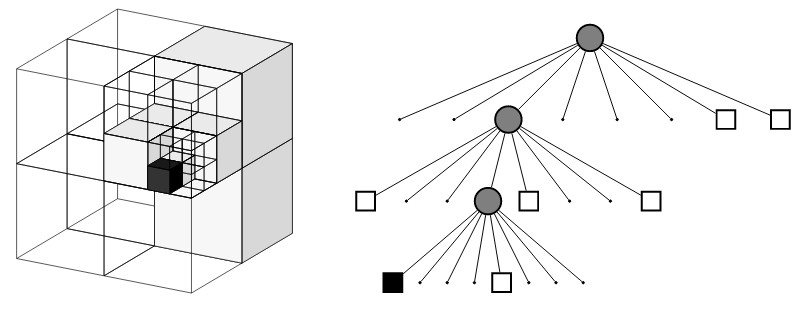
\includegraphics[width=0.5\linewidth]{images/octree.jpg}
  \caption[Représentation graphique d'une Octree]{L'octree est une structure en arbre souvent utilisé pour partitionner un espace tri-dimentionel. Figure prise de \citep{Hornung2013}.}
  \label{fig:octree}
\end{figure}

La structure Octree rend l'OctoMap particulièrement efficace en termes de mémoire comparativement à une séparation naïve de l'espace en voxels car l'arbre n'est étendu qu'au besoin. Alors que certaines représentations de l'espace utilisent une forme binaire où tout voxel est soit occupé ou libre, OctoMap utilise une forme probabiliste où chaque voxel est inconnu ou a une probabilité d'être occupé ou libre permettant donc l'OctoMap de représenter l'incertitude et le bruit de mesure sur le capteur utilisé pour construire la carte. L'OctoMap peut ensuite être utilisé par divers algorithmes de génération de trajectoire tel que les RRT ou A*.

Par contre, une OctoMap n'est pas particulièrement bien adapté aux méthodes de planification de trajectoire par optimisation qui ont besoin de savoir la distance aux obstacles en tout point de la carte ainsi que les gradients de distance \citep{ratliff2009chomp, Oleynikova2016}. Ce calcul pouvant être coûteux, \cite{oleynikova2017voxblox} propose d'utiliser une représentation des surface par des fonctions de distance signées tronquées offrant une accélération par la suite dans le calcul des champs de distance euclidiennes signées.

Dans un autre ordre d'idées \cite{Fridovich-Keil2017AtomMap} abandonnent complètement la représentation par grille et proposent d'utiliser des sphères (des \guillemotleft atômes \guillemotright) organisés dans un arbre $k$-d. Ceci permet une représentation plus précise de l'espace libre tangeant aux surfaces en plus de faire l'estimation de fonctions de distance signées en temps réel.

\section{Génération de trajectoires d'exploration et couverture de surfaces}\label{subsec:generation}

En général, le but des générateurs de trajectoire est d'optimiser une certaine métrique permettant de décider à quel endroit il faut placer le véhicule et son capteur pour faire l'inspection de la structure.

Tout d'abord, considérant le cas d'une mission sans information \textit{a priori}. Il s'agit d'une mission d'exploration où la génération de trajectoire doit se faire itérativement en temps réel pour envoyer le robot aux confins de l'espace connu. On tente en fait de répondre à la question:

\begin{quote}
  Given what you know about the world, where should you move to gain as much new information as possible? (Sachant ce que nous savons à propos du monde, où devrions nous aller pour gagner le plus d'information possible?) \citep{Yamauchi1997}.
\end{quote}

Pour ce faire Yamauchi introduit le concept de \textit{frontier-based exploration} qui cherche à guider un robot vers la frontière entre l'espace connu et libre et l'espace inconnu. Suivant cette idée plusieurs chercheurs proposent des fonctions de coût à minimiser permettant de choisir à quel endroit de la frontière explorer. \citep{Wirth2007} proposent de subdiviser une carte 2D en celulles pour lesquelles une fonction de coût est calculée en prenant en compte non seulement la plus courte distance par rapport au robot mais aussi la distance par rapport à l'obstacle le plus proche. Chaque nouvelle position objectif minimise ainsi la distance pour s'y rendre mais aussi le risque encouru par le robot. Au lieu d'utiliser les \textit{frontier} comme objectifs \citep{Dornhege2011} proposent une formulation du problème utilisant les \textit{frontier} en tant que candidats possibles d'ouvertures dans les murs qui permetteraient à une caméra de cartographier l'espace vide se retrouvant derrière.

\citep{Bircher2016} proposent une méthode d'exploration 3D basé sur l'algorithme \textit{Rapidly exploring Random Trees} (RRT) où un arbre est grandit dans l'espace ouvert connu. À chaque sommet, l'angle de vue de la caméra est utilisé pour estimer le gain exploratoire de la position. Une fois l'arbre construit, le véhicule exécute la première étape de la branche possédant le plus grand gain total. L'arbre complet est ensuite recalculé en utilisant la branche choisie comme point de départ. En d'autres mots, leur méthode tente de maximiser le gain exploratoire en prenant aussi en compte les gains futurs d'une trajectoire. Outre les gains exploratoires, certains auteurs tentent aussi de prendre en compte l'effet des trajectoires sur leurs systèmes de navigation. Par exemple \citep{Papachristos2017} améliorent la méthode de Bircher en sélectionnant un trajectoire qui permet aussi de minimiser l'incertitude sur leur système de cartographie et d'odométrie visuelle. \citep{Wirth2007} notent d'ailleurs que la proximité d'un obstacle est un danger (de collision) mais l'éloignement des obstacle en est aussi puisque la portée limitée des capteurs pourrait rendre un système de SLAM temporairement aveugle.

Alors que les méthodes précédentes se préoccupent de maximiser le gain d'information, elles ne prennent pas en compte les contraintes de temps liées à l'autonomie des robots; Un problème qui affecte grandement les véhicules aériens multi-rotors. En combinant une fonction d'entropie calculée dans un voisinage local avec le coût en distance d'une trajectoire, \citep{Wang2017} proposent une méthode d'exploration se basant sur les \textit{Information Potential Fields} (les champs de potentiels d'information). Similaire à la méthode des champs de potentiels pour l'évitement d'obstacles, le robot fini par être attiré aux régions les plus proches à haut gain d'information. Toutefois, minimiser la longueur de la trajectoire n'assure pas nécessairement une minimisation du temps d'exploration si nous prenons aussi en compte l'accélération ou le jerk requis pour exécuter celle-ci. Pour résoudre ce problème \citep{Cieslewski2017} proposent une extension de la méthode de \citep{Yamauchi1997} où le prochain \textit{frontier} choisi est sélectionné dans le champ de vision du véhicule et de tel sorte qu'il minimise le changement de vitesse requis au robot. Ainsi, la trajectoire exécutée peut être plus longue que les méthodes conventionnelles mais elle permet de maintenir une vitesse de navigation plus élevée.

Dans un autre ordres d'idée, une trajectoire complète et globalement optimale peut être générée au préalable si de l'information \textit{a priori} est disponible. Pour une mission où la géométrie de la structure à inspecter est connue \citep{Bircher2015} proposent de résoudre le problème en deux temps. En subdivisant le modèle en un maillage de triangles, on obtient pour chaque face un ensemble de points de vues admissibles. À chaque itération, des point de vus sont choisis séquentiellement en résolvant un problème d'optimisation QP où la fonction de coût minimise la distance par rapport aux points de vue voisin et où les contraintes assurent que la surface soit visible par le véhicule. Une fois l'ensemble choisi, une recherche heuristique est effectuée pour résoudre un problème du commis voyageur à travers l'ensemble. Bircher réexécute les deux étables jusqu'à ce qu'une trajectoire satisfaisante soit trouvée.

Comparativement à l'inspection par exploration (en temps réel) la génération de trajectoire hors-ligne permet de créer des plans plus optimals en termes de temps et de distance à parcourir. Par contre, cette trajectoire peut avoir un risque de collision s'il s'avère que le modèle utilisé diffère de la structure réelle, par exemple dans la cas d'un édifice partiellement endommagé par un désastre naturel ou une variation dans l'angle des pales d'une éolienne. \citep{Hepp2017} présentent un système faisant une première passe à haute altitude pour construire une carte rudimentaire dans laquelle la seconde inspection de près est planifiée suivant une maximization du gain d'information.

\section{Méthodes de navigation}\label{subsec:navigation}

Champs de potentiel

\section{Méthodes automatiques d'inspection d'éoliennes}\label{subsec:eolienne}

L'inspection d'éoliennes par UAV autonome étant une application relativement nouvelle, peu de travail a été publié à ce sujet particulier et à ce jour, la majorité du travail demeure théorique, en simulation seulement ou en environnements à petite échelle. Avant tout, \citep{Zhang2014} démontrent la faisabilité de repérer automatiquement des craques sur la surface d'une éolienne au moyen des détecteurs de bordures bien connus Canny et Sobel. Du travail préliminaire a été réalisé sur les éléments de base requis pour faire une inspection autonome. Notamment au niveau de l'utilisation du principe du flux optique pour l'estimation de la vitesse relative entre un véhicule aérien et une éolienne \citep{Hoglund2014} ainsi que l'utilisation de la transformée de Hough linéaire et de traitements géométriques pour la reconaissance automatique d'éoliennes \citep{Stokkeland2015}. Stokkeland explique qu'une inspection entièrement visuelle est difficile à réaliser dû à la grande quantité de bruit et de sources d'erreurs présentes sur le terrain. Par exemple, la segmentation entre la surface blanche de l'éolienne et les nuages en arrière plan est extrêmement sensible au réglage des paramètres du filtre de couleur. C'est pourquoi \citep{Heggem2017} fait usage de vision active au moyen d'un projecteur laser et de caméras stereo pour détecter la distance et la forme de la pale. Avec une matrice de seulement 11x11 points, Heggem parvient ensuite à calculer dans quelle direction son UAV doit se diriger pour poursuivre son inspection.

Du côté commercial, peu de compagnies se sont aventurées dans le domaine \footnote{Nous notons la présence de SkySpecs aux États-Unis, Pro-Drones en Italie et Perceptual Robotics en Angleterre.} mais tous semblent faire usage de radars lasers et de caméras sous une forme ou une autre.

\section{Traitement d'images}

\subsection{Modèle de caméra}
\label{subsec:modele_camera}

Il arrive souvent dans des applications de traitement d'image de devoir passer du domaine 3D à 2D et vice-versa. Pour ce faire, il est important de passer en revue les modèles de projection et de distortion d'images courramment utilisés. Tout point 3D $p_w$ à coordonnées connues peut être projetté sur le plan image à un point en coordonnées en pixels $\boldsymbol{x_s}$ par l'équation \ref{eq:pinhole_projection}.
\begin{align}
\boldsymbol{x_s} = K[R|t]p_w = P p_w
\label{eq:pinhole_projection}
\end{align}
On nomme la matrice $3\times4$ $P$ la matrice de caméra, la matrice $3\times3$ $K$ la matrice des paramètres intrinsèques, $R$ est une rotation othogonale et $t$ est une translation. Dépendamment des auteurs $K$ peut être posé différemment, l'équation \ref{eq:intrinsics} présente sa forme générale où $f_{[x,y]}$ sont la distance focale en pixels, $(c_x, c_y)$ le centre optique en pixels, $s$ le \textit{skew} prenant en compte l'angle possible entre les axes du capteur et les axes optiques et finalement $\alpha$ est le facteur de forme.
\begin{align}
  K = \begin{bmatrix}
  f_x & s & c_x \\
  0   & \alpha f_y & c_y \\
  0  &  0  & 1
\end{bmatrix}
\label{eq:intrinsics}
\end{align}
En pratique la majorité des application tel quel la librairie de traitement d'images OpenCV vont simplifier $K$ au moyen de $s = 0$ et $\alpha = 1$ \citep{itseez2015}. Il est aussi utile de passer aux coordonnées homogènes au moyen d'une matrice $\boldsymbol{\tilde{P}}$ $4\times4$ en ajoutant une ligne à $P$,
\begin{align}
  \boldsymbol{\tilde{P}} = \begin{bmatrix}K & \boldsymbol{0} \\ \boldsymbol{0} & 1\end{bmatrix}
  \begin{bmatrix}R & t \\ \boldsymbol{0} & 1\end{bmatrix} = \boldsymbol{\tilde{K}} \boldsymbol{E}
    \label{eq:homogeneous_projection}
\end{align}
où $\boldsymbol{E}$ est une matrice de transformée 3D. La projection se fait de la même façon qu'à l'équation \ref{eq:pinhole_projection} avec $\boldsymbol{\bar{p}_w} = \begin{bmatrix}p_w^\top & 0 \end{bmatrix}^\top$ et $\boldsymbol{x_s} = \begin{bmatrix}x_s & y_s & 1 & d\end{bmatrix}^\top$
\begin{align}
  \boldsymbol{x_s} \sim \boldsymbol{\tilde{P}} \boldsymbol{\bar{p}_w}
\end{align}
où le symbole $\sim$ indique une égalité à l'échelle et $\boldsymbol{x_s}$ doit être normalisé après la multiplication pour que la troisième composante soit $1$ \citep{Szeliski2011}.

Ces formules sont valides dans le cas de projections entièrement linéaires, par contre les systèmes optiques vont habituellement introduire une certaine distortion de l'image. Par exemple dans la Figure \label{fig:distortion} les lentilles de la caméra Zed avec un angle de vue de $110^\circ$ (D) introduisent beaucoup de distortion courbant ainsi des lignes qui devraient normalement êtres droites.

\begin{figure}[htp]
  \centering
  \begin{minipage}{0.4\textwidth}
    \centering
    
\includegraphics[width=\linewidth]{images/placeholder.png}
    (A)
  \end{minipage}
  \begin{minipage}{0.4\textwidth}
    \centering
    
\includegraphics[width=\linewidth]{images/placeholder.png}
    (B)
  \end{minipage}
  \caption{Exemple de distortion introduite par une lentille à grand angle. (A) l'image originale (B) l'image rectifiée}
  \label{fig:distortion}
\end{figure}

Plusieurs modèles de distortion ont été proposés à travers le temps mais le plus répandu est celui radial-tangentiel, radial puisqu'il dépend de la distance du pixel par rapport au centre optique et tangentiel pour le déplacement des rayons tangentiel au cercle autour du centre optique. La distortion radiale-tangentielle peut-être exprimé par un polynôme permettant de mettre en correspondance les pixels de l'image originale $(x_c, y_c)$ en coordonnées normalisées aux pixels de l'image rectifiée $(u, v)$.

\begin{equation}
\begin{aligned}
  \hat{x}_c &= x_c\left(\frac{1 + \kappa_1r_c^2 + \kappa_2r_c^4 + \kappa_3r_c^6}{1 + \kappa_4r_c^2 + \kappa_5r_c^4 + \kappa_6r_c^6}\right) + 2p_1 x_c y_c + p_2(r_c^2 + 2 x_c^2) \\
  \hat{y}_c &= y_c\left(\frac{1 + \kappa_1r_c^2 + \kappa_2r_c^4 + \kappa_3r_c^6}{1 + \kappa_4r_c^2 + \kappa_5r_c^4 + \kappa_6r_c^6}\right) + p_1 (r_c^2 + 2 y_c^2) + 2p_2 x_c y_c \\
  r_c^2     &= x_c^2 + y_c^2
  \label{eq:rectification}
\end{aligned}
\end{equation}
\begin{equation}
\begin{aligned}
  u & = f_x \hat{x}_c + c_x\\
  v &= f_y \hat{y}_c + c_y
  \label{eq:focal_scaling}
\end{aligned}
\end{equation}
Les paramètres $\kappa_{[1-6]}$ sont les coefficients de distortion radial et $p_{[1,2]}$ les coefficients de distortion tangentiel. L'équation \ref{eq:focal_scaling} permet de mettre à l'échelle les coordonnées normalisées en coordonnées en pixels. Les paramètres de distortion et intrinsèques peuvent être estimés conjointement suivant la résolution d'un problème des moindres carrés non-linéaire \citep{Zhang2000}.

Bien que le modèle radial-tangentiel soit le plus populaire, entres-autres par sa présence dans la librairie de traitement d'images OpenCV, plusieurs auteurs proposent de nouveaux modèles avec divers avantages. Par exemple le modèle de distortion équidistant proposé par \cite{Kannala2006} est apte à modéliser la distortion à la fois de lentilles normales et de lentilles ultra-grand angle et le modèle par fonction rationelle de \cite{Claus2005} adapté aux lentilles grand-angle et catadioptriques.

\subsection{Vision stereo}

\begin{figure}[h]
  \centering
  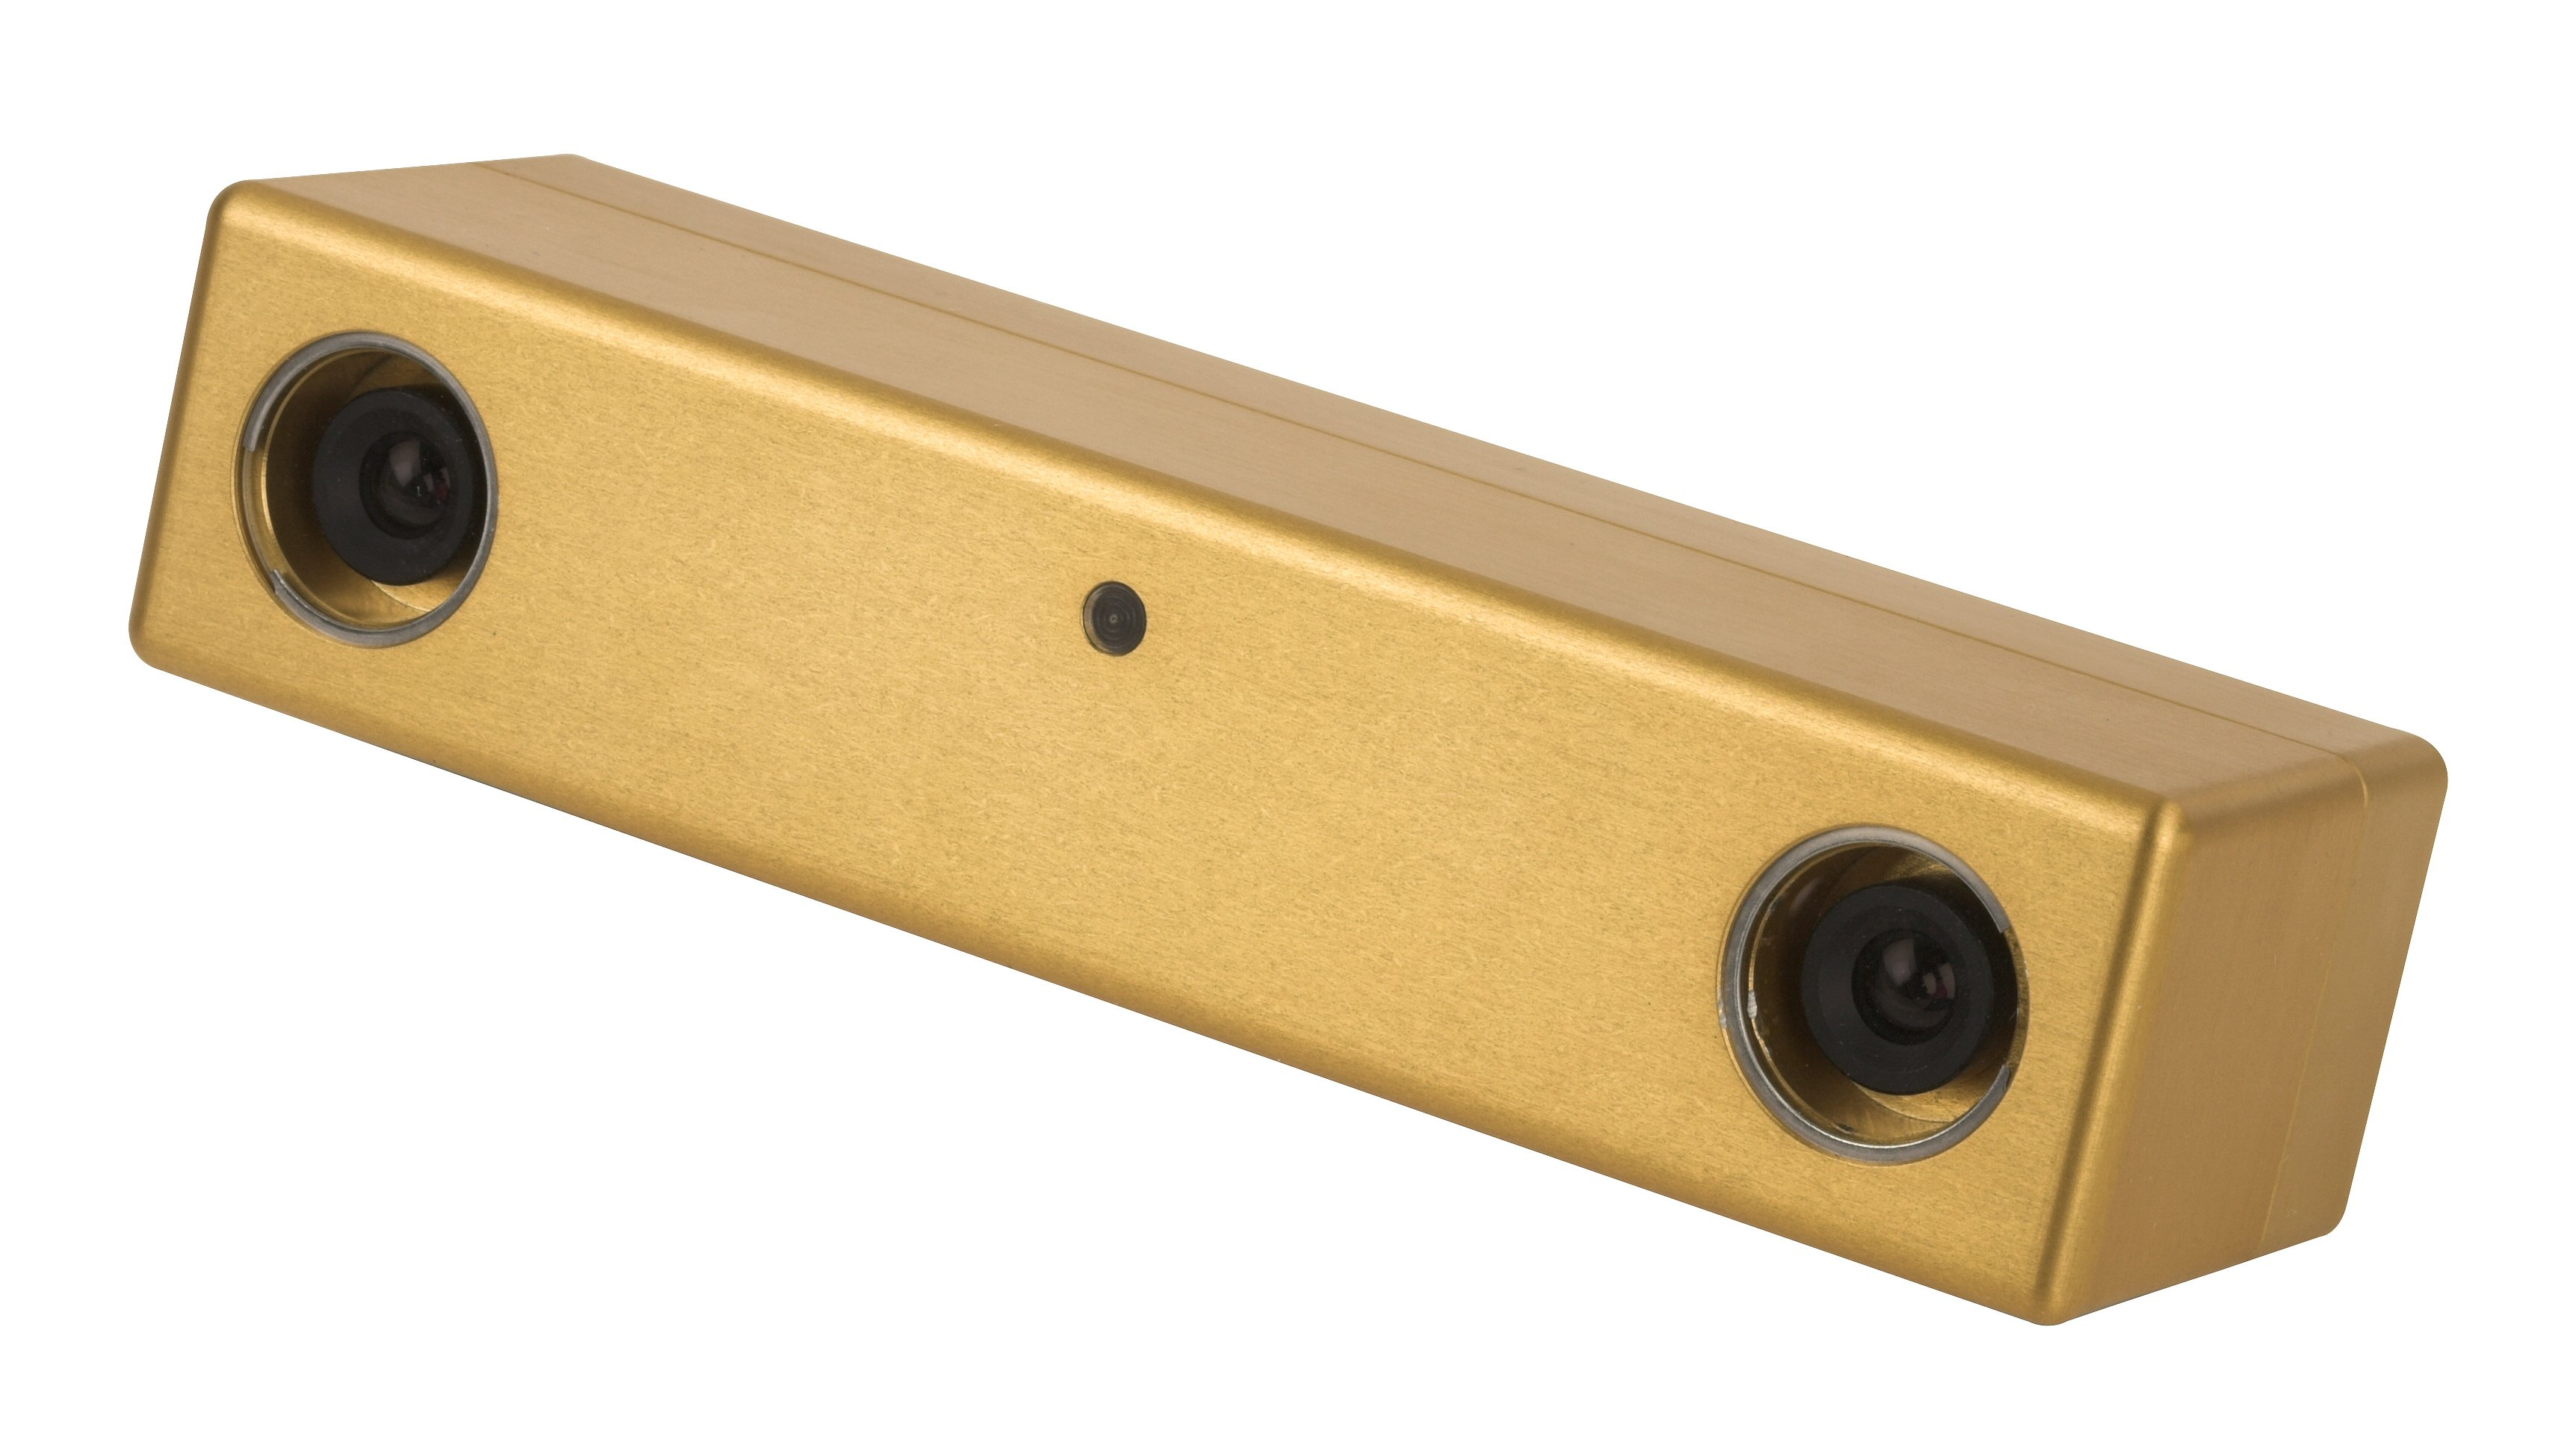
\includegraphics[width=0.5\linewidth]{images/bumblebee2.jpg}
  \caption[Exemple de caméra stereo]{Exemple de caméra stereo PointGrey Bumblebee2}
  \label{fig:stereo_camera}
\end{figure}

La vision stereo est un sujet qui est étudié depuis longtemps pour diverses utilisations tel que la cueillette d'objets par bras manipulateur \citep{Hernandez2017}, l'effacement d'arrière-plan \citep{Kanade1996Stereo} et la navigation de robots \citep{Fraundorfer2012}. Sans aller dans les détails de la géométrie épipolaire permettant de trianguler un point dans l'espace, l'idée générale derrière la vision stereo est de comparer les images de deux caméras pour calculer la distance entre deux points correspondants. Cette distance, que l'on nomme la disparité, est directement liée à la position 3D du point dans le monde selon la relation
\begin{align}
  d = f \frac{B}{Z}
\end{align}
où $d$ est la disparité, $f$ est la longueur focale en pixels, $B$ est la distance entre les deux caméras et $Z$ est la profondeur du point. Diverses méthodes existent pour mettre en correspondance les points (ou plus souvent des blocks de plusieurs pixels) entre les deux images. Nous avons par exemple les algorithmes locaux cherchant le plus petit coût de correspondance suivant une métrique tel que la différence absolue ou la somme des différences au carré calculée sur l'intensité des pixels d'un bloc \citep{Szeliski2011}. Ces coûts locaux peuvent aussi être optimisés globalement par \textit{belief propagation} pour obtenir une image de disparité cohérente \citep{Klaus2006}. L'approche utilisée dans la librairie de traitement d'images OpenCV est en fait une approximation de l'optimisation globale où la programmation dynamique est utilisé pour optimiser une fonction d'énergie \citep{Hirschmuller2008}.

Cependant, peu importe l'algorithme utilisé, il sera toujours important d'avoir de la texture dans l'image, sans quoi il existera une incertitude sur la correspondance des blocs et le calcul de disparité échouera. Outre les filtres lisseurs tentant de remplir les trous dans une image de disparité où la recherche de correspondance aurait échoué, les avancées récentes dans le domaine tendent vers l'utilisation de l'apprentissage machine pour prédire l'image de disparité en entier \citep{Kendall_2017_ICCV}. \cite{meier2017real} proposent une solution plus classique où l'échec de correspondance est prédit et corrigé au moyen d'une caméra stereo secondaire placée orthogonalement à la caméra principale.

\subsection{Détection de lignes}

La méthode la plus connue pour la détection de contours dans une image reste à ce jour celle proposée par \cite{Canny1986} qui consiste brièvement en un calcul de gradient suivit d'une suppresion des non-maxima. Avec la popularité grandissante de l'apprentissage machine, certaines nouvelles méthodes ont été proposées pour la détection de contours à base de réseau de neuronnes. Par exemple \textit{Holistically-Nested Edge Detection} proposé par \cite{Xie2015} est un réseau de neuronnes entièrement convolutionnel qui faut aussi usage d'apprentissage multi-échelle de caractéristiques imbriquées. L'avantage majeur des méthodes par apprentissage machine est qu'elles ne requirent pas la calibration de de paramètres.

Une fois les contours détectés et inscrits dans une image binarisée, il devient possible d'appliquer une transformée de Hough pour la détection de lignes droites \citep{Duda:1972}. Avec le temps, plusieurs améliorations ont été proposées pour accélérer le calcul de la transformée, nottamment l'introduction de méthodes probabilistes utilisant qu'un sous-ensemble des données pour la détection des lignes \citep{Matas2000}. \citep{Herout2013} Dénombrait 39 différentes variantes de la transformée de Hough incluant des variantes faisant usage de matériel spécialisé tel que des GPU ou des FPGA.

D'autres méthodes de détection de ligne ont aussi été proposées sans le besoin de passer par une transformée de Canny. Par exemple le \textit{Line Segment Detector} de \citep{Gioi2012lsd} fonctionnant par régions de support de ligne. D'un autre côté, EDLines proposé par \citep{AKINLAR20111633} fonctionne directement sur une image à tons de gris, des points d'ancrage sont calculés sur une image gradient pour effectuer un traçage de contours. LSD et EDLines ont tous les deux l'avantage d'être rapides et ont étés conçus pour ne pas avoir besoin de réglage de paramètres.
  % Revue de littérature.
% !TEX root = Document.tex
\Chapter{Choix de capteurs}\label{sec:capteurs}
\color{red}
Intégrer ce chapitre à la revue de littérature? Ou faire un chapitre très court.
\color{black}

\section{Systèmes passifs}

\section{Systèmes actifs}

\subsection{Time-of-flight}

\subsection{Projection laser}

\subsection{subsubsection name}
             % Premier thème (Doctorat) ou "Détails de la Solution" (Maîtrise).
\Chapter{SECOND THÈME}\label{sec:Theme2}
Texte.
             % Second thème (Doctorat) ou "Résultats théoriques et expérimentaux" (Maîtrise).
% !TEX root = Document.tex
\Chapter{Inspection d'éoliennes par UAV}\label{sec:uav}

Dans ce chapitre nous traitons du projet de l'automatisation d'inspection d'éoliennes par un véhicule aérien autonome réalisé conjointement avec la compagnie Microdrones Canada Inc.

\section{Description du problème et méthode d'inspection}

Les éoliennes doivent régulièrement être inspectées pour détecter et réparer le plus tôt possible des failles structurelles sur leurs pales qui peuvent apparaître avec le temps dû aux intempéries ou même quand elles sont frappées par la foudre. La peinture recouvrant celles-cis étant moins élastique que le composite de fibre de verre dont elles sont construites, un défaut structurel se manifeste inévitablement à la surface de la pale sous la forme de craques ou de trous. C'est pourquoi une inspection visuelle doit être régulièrement faite pour déceler et réparer toute irrégularité dans la structure avant qu'un bris catastrophique ne se produise.

En temps normal, une inspection se fait par une équipe d'une ou deux personnes devant grimper l'éolienne. D'abord, l'équipe attend que le vent fasse tourner le rotor jusqu'à ce que la pale devant être examinée pointe vers le sol. À ce moment, le frein est enclenché et l'angle d'inclinaison des pales est ajusté pour que le vent ne créé pas de couple sur le rotor. L'équipe grimpe ensuite la tour jusqu'au sommet, ce qui peut prendre une dizaine de minutes si l'ascenceur est non fontionnel, chose qui arrive fréquemment. Une fois rendu au rotor, un frein mécanique secondaire est activé pour manuellement bloquer la rotation des pales. L'équipe fait ensuite une descente en rappel le long de la pale pour faire leur inspection visuelle et tactile de la surface. Une fois l'inspection terminée le processus est recommencé pour les deux autres pales. En tout, inspecter une éolienne peut prendre entre deux et quatre heures dépendamment du nombre bris à documenter.

%En plus de prendre beaucoup de temps, les inspection d'éoliennes posent un réel risque au niveau de la santé et sécurité des travailleurs nottament à cause des chutes possibles dans la tour pouvant faire plus d'une centaine de pieds de haut ou aussi par le fait de devoir naviguer des espaces confins pour se rendre au sommet de la tour \citep{Osha2017}. Ainsi, automatiser les inspections bénéfierait directement la santé des travailleurs et permetterait de sauver du temps et de l'argent.

Certains opérateurs d'UAV offrent maintenant des services d'inspection d'éoliennes. Une caméra haute définition est montée sur un cardan stabilisateur à trois axes qui est à son tour monté sur le véhicule. Ce dernier est desfois aussi augmenté d'un télémètre permettant au pilote de savoir à quelle distance il est de la structure, chose difficile à estimer lorsque le véhicule est à 100 mètres d'altitude. Ces inspections peuvent prendre jusqu'à trois employés dont un pilote, un opérateur pour la caméra et un observateur sous l'éolienne.

Le but du projet est d'explorer les solutions possibles pour réaliser un système capable de naviguer un quadricoptère autour des pales d'une éolienne à l'aide de capteurs peu coûteux avec seulement le pilote de sécurité de présent et le moins d'information \textit{a priori} possible. Ce projet peut aussi servir de tremplin vers un projet futur dans lequel aucun humain n'interviendrait, par exemple pour une flotte d'UAV chargée d'inspecter régulièrement un parc éolien entier. Puisque maneuvrer précisément autour des pales demanderait l'usage de capteurs dépassant le budget du projet et nécessiterait que l'UAV soit équipé de capteurs de position haute précision tel qu'un GPS différentiel, nous simplifions le problème en un problème à deux dimensions où le véhicule cheche à suivre le bord d'attaque (ou le bord de fuite) des pales. Deux approches ont été développées, l'une entièrement au moyen de scanners lasers et l'autre par caméras stereo.

La mission se divise en deux phases: l'approche du rotor et le suivit de ses pales qui peuvent être gérées par une simple machine à états finis. Pour l'approche du rotor nous comparons une approche à longue distance au moyen de traitement d'images à une approche à tâtons où l'UAV remonte la tour au moyen de scanner lasers. Pour le suivit des pales, nous comparons encore une méthode par traitement d'images à une méthode de suivit à tâtons. Puisque ce projet est réalisé conjointement avec la compagnie Microdrones, le quadricoptère md4-1000 a été choisi sur lequel nous installons deux scanners lasers LeddarTech Vu8, l'un horizontal et l'autre vertical et puis une caméra stereo ZED. Il est à noter que ces capteurs ne servent qu'à la navigation de l'UAV alors que la caméra haute définition sur stabilisateur resterait le moyen par lequel prendre des photos de défauts à la surface des pales.

\begin{figure}[htp]
  \centering
  
\includegraphics[width=0.5\linewidth]{images/placeholder.png}
  \caption{Systèmes de coordonnées sur le md4-1000}
  \label{fig:md41000}
\end{figure}

\begin{table}[htp]
  \centering
  \setlength{\tabcolsep}{12pt}
  \begin{tabular}[htp]{|c|l|p{10cm}|}
    \hline
    Symbole & Nom                   & Description\\\hline
    $W$     &  \textit{World}       & Suivant la convention \textit{East-North-Up} (ENU), centré au point de décollage du véhicule avec l'axe $x$ pointant vers l'est, $y$ pointant vers le nord et $z$ pointant vers le haut.\\ \hline
    $B$     &  \textit{Body}        & Encore suivant la convention ENU, l'axe $x$ pointant vers la droite, $y$ vers l'avant et $z$ vers le haut. \\ \hline
    $\mathit{BT}$  &  \textit{Body Tangent} & Repère centré sur $B$ mais compensé pour ses angles de roulis et de tangage (mais pas de lacet). En d'autres mots, le repère ${BT}$ est donc tangent à la surface de la Terre et centré sur $B$. \\ \hline
    $\mathit{C[L,R]}$ & \textit{Camera} & Suivant la convention de représentation d'images, nous avons l'axe $x$ vers la droite, $y$ vers le bas et $z$ sortant de la caméra. Les suffixes $L$ et $R$ indiquent la caméra gauche et droite respectivement. Par souci de brièveté si le repère est écrit $C$ sans préciser la caméra gauche ou droite, il indique la caméra droite.   \\ \hline
    $\mathit{L[H,V]}$ & \textit{Laser}& Les lasers aussi suivent un repère main droite avec $x$ vers l'avant, $y$ a gauche et $z$ vers le haut. Les données de distance du laser se situe tous sur son plan $XY$. Les suffixes $H$ et $V$ indique la direction du scan, horizontal et vertical, par rapport au repère $B$. \\ \hline
    $\mathit{T}$ & \textit{Turbine} & Le système de coordonnées de la turbine est centré sur le rotor avec $x$ vers la droite (vu de devant), $y$ vers l'intérieur de la nacelle et $z$ vers le haut. \\ \hline
  \end{tabular}
  \setlength{\tabcolsep}{6pt}
  \caption{Repères présents dans le système d'inspection d'éoliennes}
  \label{table:coordinate_frames}
\end{table}

\section{Approche du rotor}

\subsection{Approche de loin}
\label{subsec:approche_loin}

L'approche à longue distance comporte plusieurs avantages dont l'absence du besoin d'information \textit{a priori} à propos du placement des pales. Avec une vue d'ensemble de l'éolienne à inspecter, il devient possible de mesurer l'angle des pales, une information cruciale qui sera exploitée lorsque l'UAV devra choisir où se diriger lorsqu'il est près du rotor. Le deuxième avantage est qu'il est possible de mesurer l'angle de lacet relatif entre l'UAV et l'éolienne, permettant ainsi de placer le véhicule perpendiculaire à la surface des pales. Cette méthode requiert tout de même la présence d'un détecteur de proximité avec une portée d'au moins 10 mètres, par contre ça reste beaucoup moins dispendieux qu'un scanner laser.

Dans cette section nous détaillons une méthode légèrement modifiée de celle de \citep{Stokkeland2015} pour détecter le centre du rotor d'une éolienne à partir d'une image. En somme les étapes restent les mêmes mais de la robustesse additionnelle est introduite au moyen d'algorithmes de regroupement, une représentation différente des pales détectées est utilisée et un filtre de Kalman non-linéaire (au lieu d'un filtre de Kalman linéaire) est proposé.

La méthode de détection du rotor se divise en 6 étapes et repose majoritairement sur des raisonnements géométriques.

%\begin{enumerate}
%  \item Prétraitement de l'image
%  \begin{enumerate}
%    \item Conversion de l'image couleur à une échelle de gris
%    \item Suppression du bruit par un filtre à convolution Gaussien
%    \item Correction du contraste par égalisation de l'histogramme
%  \end{enumerate}
%  \item Détection de contours par l'algorithme de Canny
%  \item Détection de lignes par transformée de Hough probabiliste
%  \item Trouver la tour de l'éolienne en cherchant des segments verticaux débutant au bas de l'image avec compensation de l'angle de roulis du véhicule.
%  \item Trouver les candidats de segments de pales. Ce sont les segments ayant un sommet près du plus haut point détectable de la tour.
%  \item Regroupement des segments par l'algorithme DBSCAN suivit du rejet de données aberrantes par une procédure de vote.
%  \item Moyenner les segments de pales et trouver le rotor par l'intersection du prolongement des pales.
%\end{enumerate}

\subsubsection{Étape 1: Prétraitement de l'image} Avant de commencer la détection, quelques corrections à l'image doivent être apportées. Puisque la procédure ne requiert pas de données de couleur, une conversion RGB à échelle de gris est effectuée au moyen de la transformée
\begin{align}
 Y \leftarrow 0.299 R + 0.587 G + 0.114 B
 \label{eq:rgb2gray}
\end{align}
où $Y$ est le niveau de gris du pixel entre $0$ et $255$ ce qui donne comme résultat l'image de la Figure \ref{fig:detection_pretraitement} (B). Pour éliminer la présence de bruit et atténuer les textures à haute fréquence pouvant donner lieu à une sur détection de lignes lors de la transformée de Hough, nous appliquons un filtre moyenneur 3x3 par convolution. Pour l'image floutée $F$ nous avons donc
\begin{align}
  F = \Bigg(\frac{1}{9}
    \begin{bmatrix}
      1 & 1 & 1\\
      1 & 1 & 1\\
      1 & 1 & 1
    \end{bmatrix}
  \Bigg) * H
  \label{eq:boxfilter}
\end{align}
avec le résultat visible à la Figure \ref{fig:detection_pretraitement} (C) Pour les convolutions sur les bords de l'image nous répétons la valeur du pixel du bord pour les données manquantes dans l'opération de convolution. Pour augmenter le contraste et corriger les erreures d'exposition de la caméra, une égalisation d'histogramme est appliquée. Pour l'image originale $I$ et l'image égalisée $H$ que l'on peut voir dans la Figure \ref{fig:detection_pretraitement} (D), nous avons
\begin{align}
  p_n &= \frac{\text{\# de pixels d'intensité } n }{\text{\# de pixels total}}, \ \ n = 0, \ldots, 255 \\
  H_{i,j} &= \text{floor}(255 \sum_{n=0}^{I_{i,j}} p_n)
  \label{eq:egalisation_histogramme}
\end{align}
Où floor est l'opérateur arondissant à la baisse à l'entier le plus proche.
\begin{figure}[htp]
\centering
\begin{minipage}{0.49\textwidth}
  \centering
  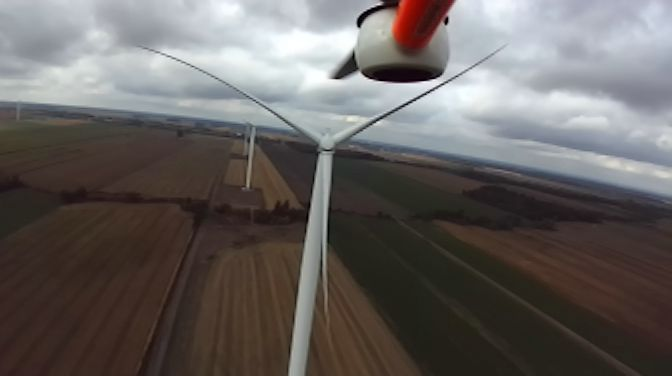
\includegraphics[width=\linewidth]{images/preprocess_original.png}
  (A)
\end{minipage}
\begin{minipage}{0.49\textwidth}
  \centering
  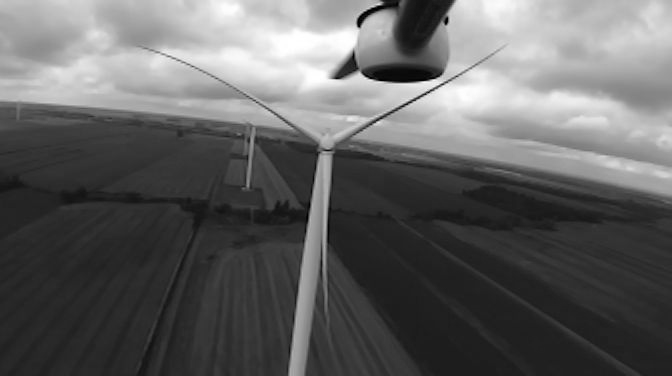
\includegraphics[width=\linewidth]{images/preprocess_gray.png}
  (B)
\end{minipage}
\vskip 1em
\begin{minipage}{0.49\textwidth}
  \centering
  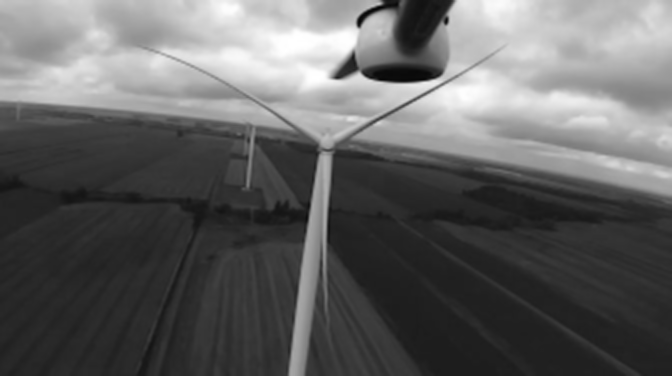
\includegraphics[width=\linewidth]{images/preprocess_blur.png}
  (C)
\end{minipage}
\begin{minipage}{0.49\textwidth}
  \centering
  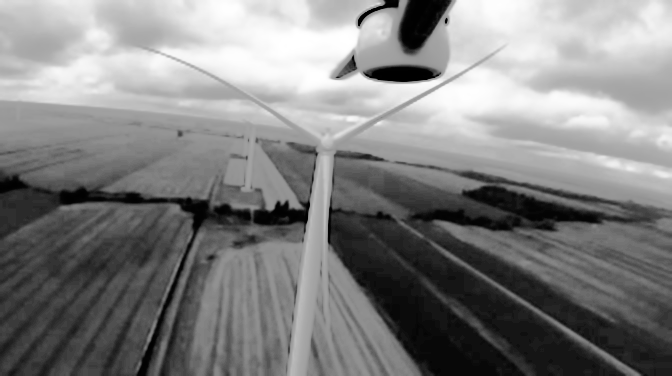
\includegraphics[width=\linewidth]{images/preprocess_histogram.png}
  (D)
\end{minipage}
\caption{(A) Image originale (B) Image en tons de gris (C) Image floutée par un filtre moyenneur (D) Image avec égalisation d'histogramme}
\label{fig:detection_pretraitement}
\end{figure}

\subsubsection{Étape 2: Détection de contours}
La détection de contours se fait au moyen de l'algorithme de \citep{Canny1986} et résultat de la procédure est visible dans la Figure \ref{fig:canny}.

% qui à son tour se fait en une série de 4 étapes:
%
% \begin{enumerate}
%   \item Un filtre Gaussien par convolution est appliqué pour atténuer le bruit. Pour générer un masque Gaussien $H$ en deux dimensions il suffit de suivre l'équation:
%   \begin{align}
%     H_{ij}= \frac{1}{2\pi\sigma^2}\exp \left(-\frac{(i-(k+1))^2+(j-(k+1))^2}{2\sigma^2} \right) ; 1 \leq i, j \leq (2k + 1)
%   \end{align}
%   où $k$ est la taille du masque, $\sigma$ est l'écart type de la distribution et $i$ et $j$ sont les indexes de rangée et de colonne respectivement. Pour $k = 5$ et $\sigma = 1.4$ nous avons
%   \begin{align}
%     I_{\text{floue}} = \frac{1}{159} \begin{bmatrix}
%       2 & 4 & 5 & 4 & 2\\
%       4 & 9 & 12 & 9 & 4\\
%       5 & 12 & 15 & 12 & 5\\
%       4 & 9 & 12 & 9 & 4\\
%       2 & 4 & 5 & 4 & 2
%     \end{bmatrix} * I_{\text{originale}}
%   \end{align}
%   \item Pour chaque pixel le gradient $G$ et l'angle du gradient $\Theta$ est calculé à partir des quantitées $G_x$ le gradient horizontal et $G_y$ le gradient vertical suivant les équations:
%   \begin{align}
%     G_x =  \begin{bmatrix} -1 & 0 & 1 \\
%     -2 & 0 & 2 \\
%     -1 & 0 & 1
%   \end{bmatrix} * I_{\text{floue}}
%   \end{align}
%   \begin{align}
%     G_y = \begin{bmatrix}
%     -1 & -2 & -1\\
%     0 & 0 & 0 \\
%     1 & 2 & 1
%   \end{bmatrix} * I_{\text{floue}}
%   \end{align}
%   \begin{align}
%     G = \sqrt{G_x^2 + G_y^2}
%   \end{align}
%   \begin{align}
%     \Theta = \atantwo(G_y^2, G_x^2)
%   \end{align}
%   \item Une suppression des non-maxima est appliquée. Pour un pixel de l'image gradient $G_{ij}$ nous comparons la valeurs aux deux pixels adjacents dans les directions $\pm\Theta$, si la valeur de $G_{ij}$ est plus grande que les deux autres, il est gardé, sinon il est mit à $0$.
%   \item Un double seuil, l'un haut $T_h$ et l'autre bas $T_b$, est appliqué par hystérésis pour atténuer les pixels de contours trop faibles. Un pixel $G_{ij}$ plus fort que $T_h$ est marqué comme un pixel au contour fort. Les pixels plus faibles que $T_b$ sont supprimés (mise à $0$). Les pixels entre les deux sont gardés seulement s'ils sont adjacents à un pixel fort. Canny suggère que le ratio $T_b$ à $T_h$ soit entre $1:2$ et $1:3$.
% \end{enumerate}

\begin{figure}[htp]
  \centering
  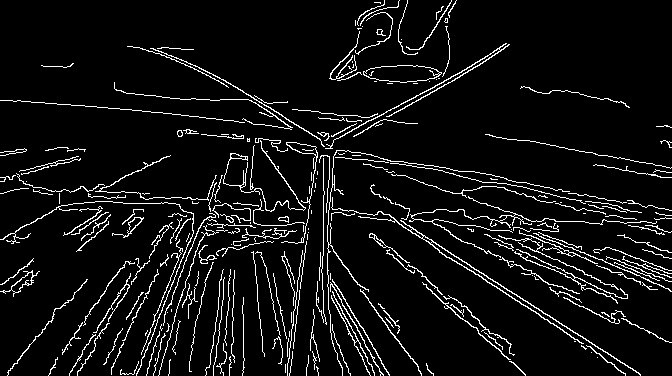
\includegraphics[width=0.6\linewidth]{images/canny.png}
  \caption{Résultat de l'application du filtre de Canny avec $T_b = 27$ et $T_h = 81$}
  \label{fig:canny}
\end{figure}

Outre la méthode de Canny, il existe des méthodes modernes plus performantes que celle de Canny, par exemple \citep{Xie2015} proposent un réseau de neuronnes entièrement convolutionel capable de détecter beaucoup mieux les contours, et ce, sans avoir à manuellement ajuster des paramètres. Par contre dans nos tests, la haute précision de la méthode retournait trop de données et il devenait difficile de passer aux prochaines étapes de la détection.

\subsubsection{Étape 3: Détection de lignes}

Une fois les contours trouvés, nous pouvons les utiliser pour détecter des segments de droite dans l'image. Dans le cas où des parties du véhicule sont visibles dans l'image, il suffit d'appliquer un masque avant de débuter cette étape. Pour trouver les segments, nous appliquons la transformée de Hough probabiliste \citep{Matas2000} pour détecter des segments de droites dans l'image de contours.

\subsubsection{Étape 4: Recherche de la tour}
\label{subsubsec:approach4}

Stokkeland explique que la partie la plus facile à détecter est la tour puisqu'elle est toujours verticale et répond fortement à la détection de lignes. Pour la trouver, il suffit de chercher une ligne verticale (compensée pour l'angle de roulis de l'UAV) dont l'un des sommets repose dans le base de l'image. Puisqu'il arrive parfois que la détection de ligne défait la tour en plusieurs segments, une fois le segment initial choisit on recherche aussi des prolongements de ce segment à une certaine distance du plus haut sommet.

\subsubsection{Étape 5: Recherche des pales}

À la fin de l'étape 4 nous avons un ensemble de segments appartenant à la tour. À partir du plus haut point de ces segments nous recherchons tout autre segment ayant un sommet dans un certain rayon du point. Ces segments sont considérés en tant que candidats à être des segments d'une pale.

Nous divergeons de la méthode proposée par Stokkeland où il tente de regrouper les segments selon l'angle par rapport à la tour; Au travers d'une procédure vorace simple où un nouveau groupe est créé lorsqu'un segment est à un angle au dessus d'un certain seuil du groupe courant. Nous notons que ceci fonctionne acceptablement sur le jeu de données à Stokkeland où le ciel est clair et son éolienne est sur une colline près de la mer, mettant donc l'horizon bien en dessous du rotor. Lors de nos essais tant en simulation que sur le terrain, nous avons noté que l'horizon était très proche de rotor donnant lieu à une grande présence de segments près du rotor faussant ainsi les résultats de la recherche de pales. C'est pourquoi nous implémentons l'étape 5 avec un algorithme de groupage formel qui inclut la résistance au bruit de mesure nommé \textit{Density-based spatial clustering of applications with noise} (DBSCAN) proposé par \citep{Ester1996}.

La particularité de DBSCAN par rapport à d'autres algorithmes de partionnage tel que $k$-means est que nous n'avons pas à fournir le nombre $k$ de partitions recherchées. À la place, nous fournissons que deux paramètres $\epsilon$ (eps) la distance d'un point à son entourage et MinPts le nombre minimum de points pour qu'une partition soit formée. Pour chaque segment, nous projettons leur angle par rapport à la tour sur un cercle unitaire. Ceci permet d'exécuter DBSCAN dans un espace euclidien pour regrouper les segments adjacents.

Une fois les groupes formés, Stokkeland utilise une stratégie de vote pour éliminer les fausses détections. La moyenne des angles est calculée et une procédure de vote débute s'il y a plus de 2 groupes. Nous choisissons 2 au lieu de 3 tel que proposé par Stokkeland pour prendre en compte le cas où 1 pale est vis-à-vis la tour. Sachant que les éoliennes ont toujours 3 pales espacées de $120$ degrés, chaque groupe calcule sa distance angulaire par rapport aux autres et vote pour les groups n'étant pas à $120$ degrés de eux-mêmes. Dans le cas où DBSCAN ressort que 2 groupes, la direction de la troisième pale est approximée à 120 degrés des deux autres pales.

\subsubsection{Étape 6: Recherche du rotor et filtrage}

L'étape 5 nous a donc fournis 3 groupes de segments représentant chacuns les pales de l'éolienne. Le centre do rotor peut donc être calculé en moyennant chaque groupe puis en prenant la moyenne de l'intersection des prolongements de chaque segment.

\begin{figure}[htb]
  \centering
  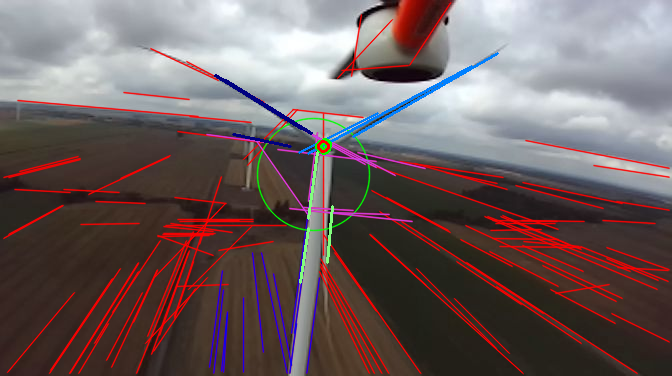
\includegraphics[width=0.8\linewidth]{images/turbine_detect_result.png}
  \caption{Résultat d'une détection réussis à la fin de la procédure.}
  \label{fig:detect_result_step6}
\end{figure}

Dans la Figure \ref{fig:detect_result_step6} nous pouvons observer les étapes $3$ à $6$ en opération. Toutes les lignes sont le résultat de la transformée de Hough appliqué à l'image des bordures suite à l'application de l'algorithme de Canny. Au bas de l'image, les lignes mauves sont les candidats à être des lignes de la tour. Elles se font rejettées cas elle ne s'étendent pas assez haut dans l'image. Le grand cercle vert est celui tracé au plus haut point de la tour dans lequel les segments de pales sont recherchées. Les segments roses sont les candidats de pales rejettés par l'algorithme de partitionnage DBSCAN et la procédure de vote.
%C'est ici que nous voyons l'amélioration de l'algorithme par rapport à Stokkeland où malgré la grande quantité de segments provenant de l'arrière plan, les pales sont quand même bien choisies.
Les pales finales sont indiquées par les lignes bleus, bleu foncé et vert pâle. Finalement, avec l'application des étapes $5$ et $6$ on peut voir que l'intersection des pales croise bien sur le centre du rotor.

Le point détecté est ensuite entré dans un filtre de Kalman linéaire permettant ainsi de garder un estimé de la position du rotor dans l'image lorsque la détection échoue. Le vecteur d'état $\boldsymbol{x}_k$ contient la position et la vitesse de déplacement en coordonnées image du centre du rotor. La matrice de transition $\boldsymbol{F}_k$ contient les termes $\gamma_x, \gamma_y \in [0, 1]$ faisant décroitre la vitesse exponentiellement avec le temps. Ceci empêche l'estimé de diverger à l'infini quand aucune mesure n'entre dans le filtre pendant de longues périodes de temps.
\begin{align}
  \begin{sbmatrix}{\boldsymbol{x}_k}u \\ v \\ \dot{u} \\ \dot{v}\end{sbmatrix} =
  \begin{sbmatrix}{\boldsymbol{F}_k}
    1 & 0 & 1 & 0\\
    0 & 1 & 0 & 1\\
    0 & 0 &  \gamma_x & 0\\
    0 & 0 & 0 &  \gamma_y
  \end{sbmatrix} \begin{sbmatrix}{\boldsymbol{x}_{k-1}}u \\ v \\ \dot{u} \\ \dot{v}\end{sbmatrix}
  + \boldsymbol{w}_k
\end{align}
où $\boldsymbol{w}_k$ est un bruit blanc Gaussien. Le modèle de mesure inclut seulement la détection du point dans l'image.
\begin{align}
  \begin{sbmatrix}{\boldsymbol{z}_k}z_x \\ z_y\end{sbmatrix} =
  \begin{sbmatrix}{\boldsymbol{H}_k}
    1 & 0 & 0 & 0\\
    0 & 1 & 0 & 0
  \end{sbmatrix} \begin{sbmatrix}{\boldsymbol{x}_{k}}u \\ v \\ \dot{u} \\ \dot{v}\end{sbmatrix}
  + \boldsymbol{v}_k
\end{align}
Le terme d'entrée de commande $\boldsymbol{u}_k$ pourrait être utilisé pour prendre en compte les vitesses angulaires commandées au robot, par contre sachant qu'il ne seront pas disponibles par télémétrie dans le md4-1000 nous ne les prenons pas en compte. La meilleure façon d'améliorer le filtre serait d'ajouter une mesure de $\dot{u}$ et $\dot{v}$, chose qui pourrait être faite par des méthodes de calcul de flux optique.

Une fois le point $(u,v)$ dans l'image trouvé, il suffit d'appliquer le modèle de caméra sténopé de la section \ref{subsec:modele_camera} et sa matrice de paramètre intrinsèques $K$ pour obtenir un vecteur unitaire $u_C$ dans le repère caméra pointant vers le rotor. Puisque la distance entre l'UAV et le rotor est beaucoup plus grande que la distance entre la caméra ($C$) et le centre du véhicule ($B$) nous pouvons la négliger. Ce qui implique que nous pouvons appliquer quelques rotations pour remettre ce vecteur unitaire dans le système d'axes $W$ (centré sur $B$) à partir de $C$ pour obtenir $u_W$.

Pour se rendre au rotor, il suffit donc de commander une vitesse dans la direction $u_W$. Puisque nous n'avons pas de mesure de distance entre l'éolienne et l'UAV la vitesse demeure constante, elle peut être régulée que lorsque la surface entre dans la portée du capteur de proximité.

\subsection{Approche en remontant la tour}
\label{subsec:laser_tower}

Dans cette méthode le véhicule est placé à proximité de la tour de telle sorte que le scanner laser puisse capter la forme de la tour et de la discontinuité introduite à l'endroit où la tour rencontre le rotor. Cette méthode est plus simple et plus fiable que l'approche visuelle mais elle repose sur deux suppositions:
\begin{enumerate}
  \item Le véhicule est bien placé par l'opérateur devant l'éolienne de tel sorte les capteurs seront perpendiculaires au plan sur lequel les pales reposent.
  \item Aucune pale n'est placée ni proche, ni devant la tour et l'angle de chaque pale est connu d'avance.
\end{enumerate}

Le principe opérationel est simple et illustré dans la Figure \ref{fig:approach}, le scanner laser horizontal est utilisé pour centrer l'UAV devant la tour et garder une distance de sécurité alors que le scanner vertical est utilisé pour détecter le rotor. Pour ce faire il faut tout d'abord projetter le vecteur de distances à un nuage de points 3D au moyen de l'équation \ref{eq:scan2cloud} où $r_i$ est une distance, $\theta_i$ est l'angle correspondant à la mesure $i$ et $n$ est le nombre de mesures retournées par le laser.
\begin{align}
  {p_{L}}_i = \begin{bmatrix}
    {{p_L}_i}_x \\
    {{p_L}_i}_y \\
    {{p_L}_i}_z
  \end{bmatrix} = \begin{bmatrix}r_i \cos \theta_i \\ r_i \sin \theta_i \\ 0 \end{bmatrix} & \text{ où } i=1,\ldots,n
    \label{eq:scan2cloud}
\end{align}
\begin{figure}[htp]
  \centering
  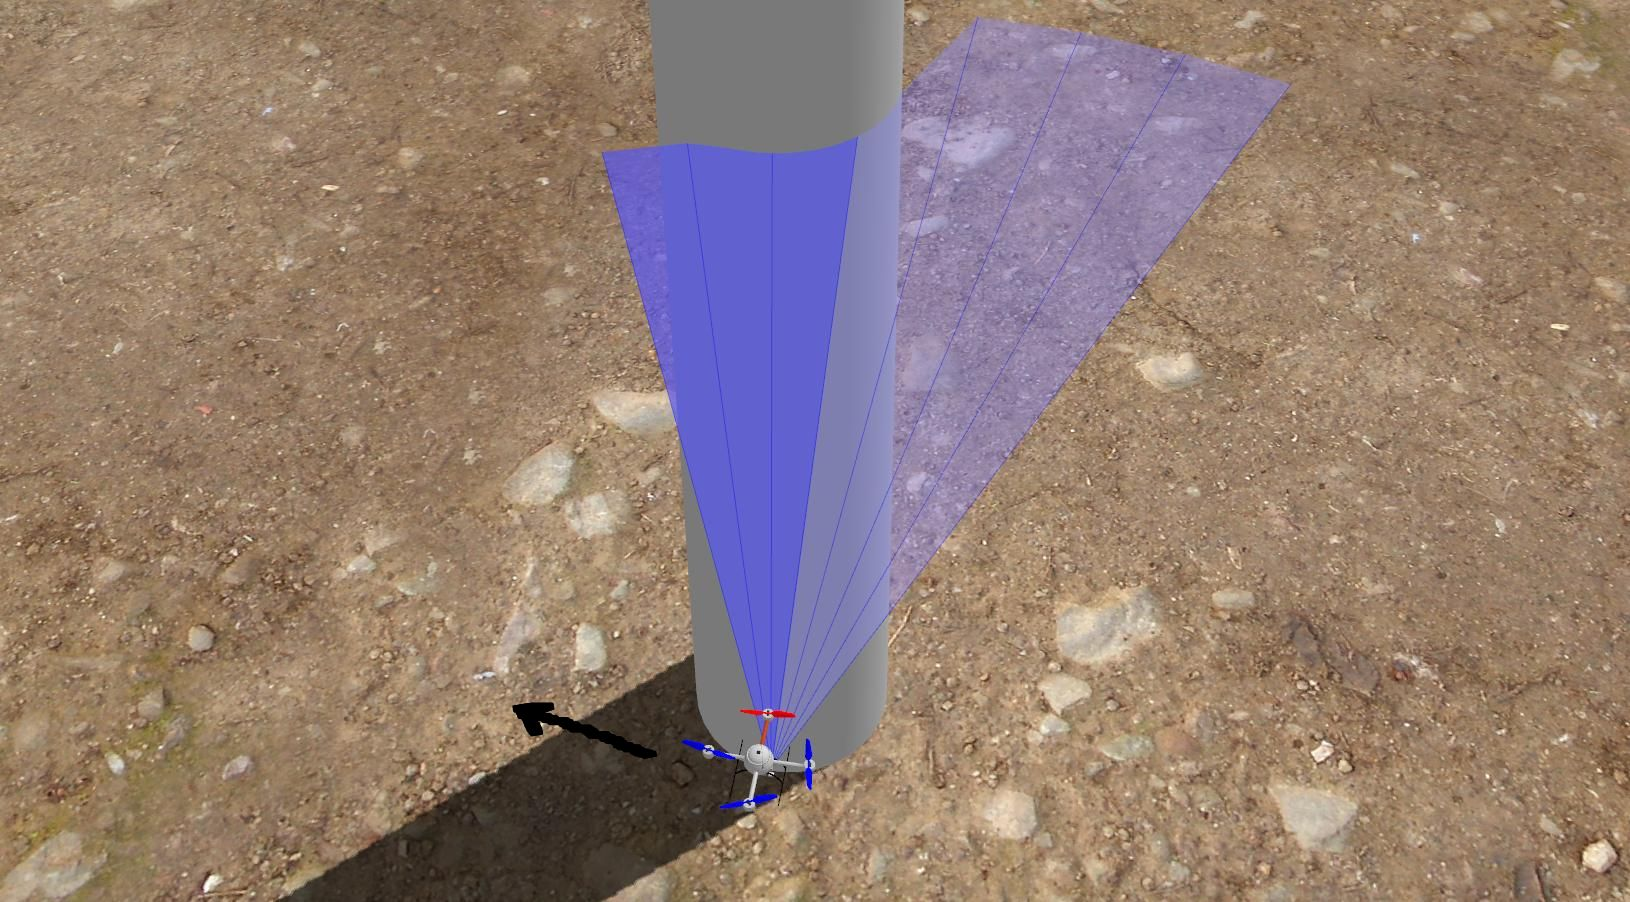
\includegraphics[width=0.8\linewidth]{images/principe_operation.jpg}
  \caption{Principe d'opération de l'approche du rotor par laser.}
  \label{fig:approach}
\end{figure}
L'équation \ref{eq:scan2cloud} nous donne des points dans le repère du laser correspondant, puisque les matrices de transformées homogènes $T_{LH}^B$, $T_{LV}^B$ ainsi que la rotation $R_B^{BT}$ sont connues, il suffit de transformer chaque $p_L$ au repère ${BT}$ suivant l'équation \ref{eq:pointcloud_bodytangent}.
\begin{align}
  \begin{bmatrix}{p_{BT}}_i \\ 1\end{bmatrix} = \begin{bmatrix}
    R_B^{BT} & 0 \\
    0 & 1
  \end{bmatrix} T_{L}^B\begin{bmatrix}{p_{L}}_i \\ 1\end{bmatrix}
  \label{eq:pointcloud_bodytangent}
\end{align}

Une fois ces mesures transformées dans le bon repère nous pouvons appliquer une loi de contrôle PID sur les axes $x$ et $y$ en plus d'une vitesse constante $v_z$ en $z$ pour calculer la commande de vitesse $u(t)$ dans le repère ${BT}$ à envoyer à l'UAV tel que présenté dans l'équation \ref{eq:tower_pid}.

\begin{align}
  u(t) = \begin{bmatrix}v_x(t)\\ v_y(t)\\ v_z(t)\end{bmatrix} =
  \begin{bmatrix}{K_p}_x e_x(t)\\ {K_p}_y e_y(t)\\ v_z\end{bmatrix} +
  \begin{bmatrix}{K_d}_x \dot{e}_x(t)\\ {K_d}_y \dot{e}_y(t)\\ 0\end{bmatrix} +
  \begin{bmatrix}{K_i}_x \int e_x dt\\ {K_i}_y \int e_y dt\\ 0\end{bmatrix}
  \label{eq:tower_pid}
\end{align}
\begin{align}
  e_x = \frac{1}{n} \sum_{i = 1}^n {{p_{BT}}_i}_x
  \label{eq:error_x}
\end{align}
\begin{align}
  e_y = d - {\text{min}}({{p_{BT}}_i}_y)
  \label{eq:error_y}
\end{align}

L'équation \ref{eq:error_x} présente le terme d'erreur $e_x$ calculé en moyennant la composante $x$ des points ${p_{BT}}_i$ provenant du laser horizontal pour déterminer si l'UAV doit bouger vers sa gauche ou sa droite pour se centrer devant la tour. L'équation \ref{eq:error_y} présente le terme d'erreur $e_y$ qui prend la plus petite mesure en $y$ pour savoir la distance par rapport à la surface de la tour et $d$ est la distance de sécurité à garder par rapport à la tour.

La détection du rotor se fait au moyen d'une détection de discontinuité en faisant une convolution (voir l'équation \ref{eq:gaussian_derivative_conv}) de la composante $y$ des points du laser vertical avec un filtre à dérivée de Gaussienne $\Gamma(x)$ discrétisé sur $n$ points pour $x=[-5\sigma,5\sigma]$ généré par l'équation \ref{eq:gaussian_derivative}. Une discontinuité est détectée si la réponse $r$ du filtre est plus haut qu'un certain seuil à déterminer de façon empirique.
\begin{align}
  \Gamma(x) = - \frac{x}{\sigma^3 \sqrt{2\pi}} \exp\left(\frac{-x^2}{2 \sigma^2}\right)
  \label{eq:gaussian_derivative}
\end{align}
\begin{align}
  r = {p_{BT}}_y * \Gamma(x)
  \label{eq:gaussian_derivative_conv}
\end{align}
Pour contrer le bruit de mesure et s'assurer que la détection est valide, le véhicule s'arrête que si la détection s'active plusieurs fois dans un certain lapse de temps. Un exemple de résultat en simulation est démontré dans la Figure \ref{fig:step_result}. Le masque de convolution est de taille $1\times8$ et $\sigma = 0.5$.

\begin{figure}[htp]
  \centering
  \begin{minipage}{0.4\textwidth}
    \centering
    
\includegraphics[width=\linewidth]{images/placeholder.png}
  \end{minipage}
  \begin{minipage}{0.4\textwidth}
    \centering
    
\includegraphics[width=\linewidth]{images/placeholder.png}
  \end{minipage}
  \caption{Résultat de la convolution sur un exemple de mesure.}
  \label{fig:step_result}
\end{figure}

\section{Suivit des pales}

Une fois devant le rotor le véhicule utilise l'information sur l'angle des pales acquise au préalable (visuellement ou par entrée utilisateur) pour savoir dans quelle direction se diriger. Il est important à cette étape de garder une grande distance de sécurité ($d_{grand} = 8$m ou plus) du rotor puisque celui-ci, constitué de multiples lignes électriques hautes tension et d'une grande quantité de métal, peut causer de l'interférence magnétique avec le magnétomètre de l'UAV qui peut potentiellement résulter en une perte de l'orientation. Cette distance peut être diminuée à $d_{petit} = 4$m lors du suivit une fois que le véhicule commence à s'éloigner du rotor.

Dans l'étape de suivit des pales, le principe est similaire à la montée de la tour, le robot cherche à suivre la pale à une vitesse constante tout en restant à une distance désiré de la pale. Nous présentons deux approches possibles, la première dans la Section \ref{subsec:pcl_blade} par nuage de point applicable à des scanner lasers 3D ou un capteur par vision active, la deuxième dans la Section \ref{subsec:laser_blade} usant que de scanner laser 2D.
%et la troisième dans la Section \ref{subsec:visual_blade} fonctionnant que visuellement.
Suivant la machine à états de la mission, une fois la fin de la pale détectée, le robot revient aux coordonnées GPS où le rotor a été détecté initialement. Puisque les pales d'une éolienne sont droites ou courbent vers l'avant, une trajectoire en ligne droite entre la fin de la pale et le devant du rotor est garantie d'être libre d'obstacles.

\subsection{Suivit par nuage de points}
\label{subsec:pcl_blade}

Dans cette méthode nous reprenons l'algorithme proposé dans le Chapitre \ref{sec:ugv} pour le suivit de mur par UGV. L'algorithme est d'ailleurs plus simple puisqu'il n'y aucun sol à filtrer du nuage de points, cependant l'avantage majeur de cette méthode est que avec le calcul de la normale de la surface il devient possible de toujour placer le véhicule perpendiculaire à celle-ci, améliorant ainsi la qualité des images prises pendant l'inspection.

\begin{figure}[htp]
  \centering
  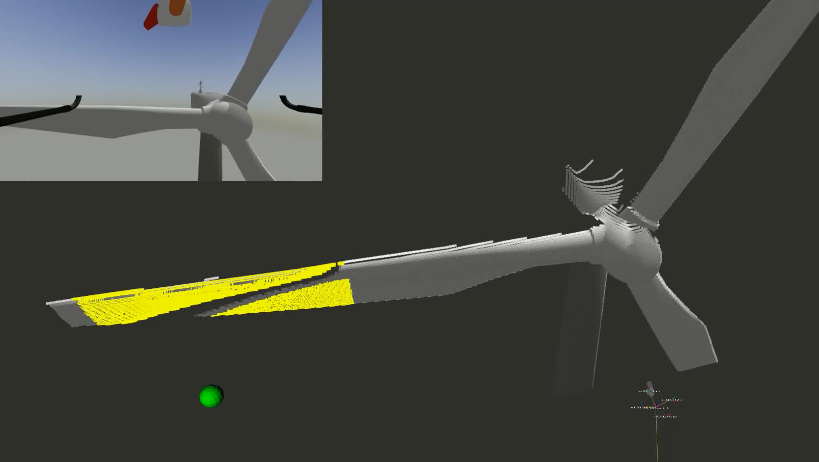
\includegraphics[width=0.7\linewidth]{images/suivit_nuage_points.png}
  \caption{Exemple de suivit de pale par nuage de points.}
  \label{fig:pcl_blade_follow}
\end{figure}

La fin de la pale est détecté de la même façon qu'un mur à angle aigü est détecté dans la section \color{red}XXX\color{black}. À mesure que le véhicule avance vers la fin de la pale, le nuage de points $\mathcal{S}$ devient de plus en plus petit, ainsi il devient possible de détecter la fin une fois que $\mathcal{S}$ passe un certain seuil. Dans la Figure \ref{fig:pcl_blade_follow} les points blancs sont le nuage de point perçu par l'UAV alors que les points jaunes représentent la tranche sélectionnée $\mathcal{S}$. La boule verte est la commande de position envoyée à l'UAV, perpendiculaire à $\mathcal{S}$.

\subsection{Suivit par scanner laser 2D}
\label{subsec:laser_blade}

Le suivit par scanner laser se fait de la même façon que la montée de la tour au moyen de deux scanner lasers perpendiculaires l'un à l'autre. Suivant les mêmes formules de projection 2D à 3D présentées dans la section \ref{subsec:laser_tower} le véhicule tente de se centrer par rapport à la pale en moyennant les points du nuage résultant tout en appliquant une vitesse constante $V_C$ dans la direction estimée de suivit. Dépendamment de l'angle de la pale seulement l'un des deux lasers est utilisé pour le suivit.

La loi de controle est donc encore un PID où les termes d'erreurs sont calculés à partir de la projection laser et la sortie est une commande de vitesse dans le repère ${BT}$.

\begin{align}
  u(t) = V_C(t) + K_P e(t) + K_D\dot{e}(t) + K_I\int{e(t)dt}
  \label{eq:pid_laser_blade}
\end{align}
$e(t)$ est calculé différemment selon la direction de la pale, en pratique, on peut utiliser la moyenne du laser horizontal si la pale est à $\pm15^{\circ}$ de la verticale et le laser vertical dans tous les autres cas. Pour une pale horizontale nous aurions par exemple
\[
e(t) = \begin{bmatrix}e_x(t) \\ e_y(t) \\ e_z(t)\end{bmatrix} =
\begin{bmatrix}
0 \\ d - \min(p_{{BT}_{i_y}}) \\ \frac{1}{n}\sum_{i=1}^{n}p_{{BT}_{i_z}}
\end{bmatrix} \text{ avec } i=1,\ldots,n
\]
Dans le cas où une erreur de capteur survient, par exemple si la pale devient assez mince pour passer entre deux rayons du laser, on répète la commande de vitesse précédente $u(t) = u(t-1)$. Ceci implique qu'une fois que le véhicule passe la fin de la pale, il continuera à voler dans le vide. La détection de fin de pale se fait donc aisément en comptant le nombre de lectures vides dans un certain lapse de temps avec un seuil à ajuster en prenant en compte que des lectures vides peuvent survenir pendant le suivit de la pale.

% \subsection{Suivit visuel pur}
% \label{subsec:visual_blade}
%
% \color{red}
% XXX drop this section?
% \color{black}

\clearpage
\section{Implémentation}

Pour l'implémentation la majorité de l'effort de développement a été dédié à l'approche purement par scanner laser suivant les sections \ref{subsec:laser_tower} et \ref{subsec:laser_blade} puisqu'elles s'avèrent à être les plus fiables, dépendent moins de paramètres à ajuster manuellement et sont peut coûteuses en termes de matériel comparé à une approche par scanner laser 3D. Le suivit par nuage de point de la section \ref{subsec:pcl_blade} a aussi été implémenté séparement pour nour permettre de vérifier la possibilité d'utiliser un capteur de profondeur. Cependant, nous posons l'hypothèse que cette méthode ne fonctionnerait pas avec une caméra stereo dût à la surface sans texture de l'éolienne ni avec un capteur fonctionnant par \textit{Time of Flight} de par leur portée limitée.
%Nous prouverons plus tard tant en simulation que sur le terrain qu'une approche par camera stereo n'est pas viable pour ce problème.
De plus, nous implémentons aussi la méthode de Stokkeland modifée décrite à la section \ref{subsec:approche_loin} pour la détection du rotor mais en vu des mauvais résultats obtenus nous n'avons pas poursuivi l'implémentation du contrôleur correspondant.

La simulation est donc développée en prévision d'un quadricoptère md4-1000 de Microdrones équipé de deux lidar LeddarVu8 de LeddarTech, une camera stereo Zed de ZedLabs et un ordinateur de bord Nvidia TX2. Les lidars Vu8 ont été sélectionnés avec un angle de vu de $48^{\circ}$ et ont la propriété particulière d'émettre des segments au lieu de faisceaux collimatés de la même manière que les lidars traditionnels. Par conséquent il devient improbable en pratique qu'une pale d'éolienne puisse se perdre entre deux rayons du lidar.

%Le md4-1000 possède une interface de communication mdSI$^{2}$ (\textit{System Integrator Interface}) permettant de recevoir la télémétrie du robot et de lui envoyer des commandes de vitesse dans le repère $BT$.
L'entièreté du logiciel a été développé en C++ à l'aide de l'interlogiciel
Robot Operating System\footnote{http://www.ros.org/} (ROS) incluant les pilotes pour les divers capteurs et la communication par UART au md4-1000. Le traitement d'images repose sur la librairie OpenCV \citep{itseez2015} et la machine à états faisant la gestion de la mission, présentée dans l'annexe \ref{annexe:state_machine}, a été écrite à l'aide de la librairie Boost \textit{Meta State Machine} \citep{Schling2011}. En tout temps la machine, que l'on nomme \code{Commander} garde un pointeur vers un objet implémentant l'interface \code{ControllerInterface}. Ces contrôleurs sont instanciés et détruits dynamiquement à chaque changement d'état, nous permettant ainsi d'avoir accès à une grande quantité de contrôleurs spécifiques tout en gardant l'utilisation de la mémoire vive à un minimum. Le \code{Commander} calcule les commandes de vitesse à une fréquence de $50$Hz, la même que la fréquence maximale de l'odométrie. Quand une mise à jour d'odométrie ou des lidars est reçue elle est mise dans un tampon en attente du prochain cycle de calcul.

\begin{figure}[htbp]
  \centering
  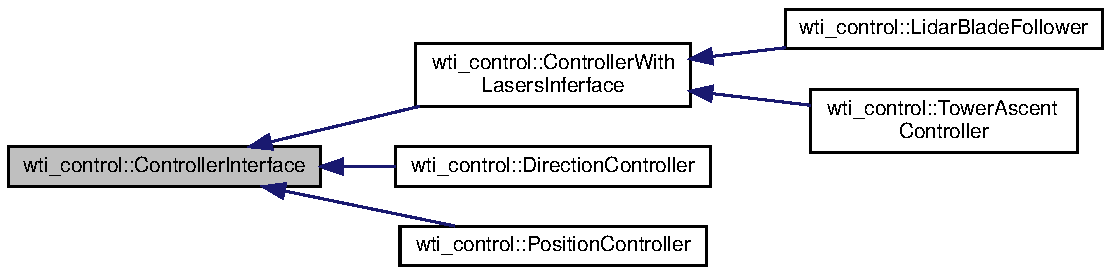
\includegraphics[width=\linewidth]{images/uml_controller.pdf}
  \caption{Diagramme de classe des différents contrôleurs utilisés par la machine à états.}
  \label{fig:uml_controller}
\end{figure}

La Figure \ref{fig:uml_controller} présente les contrôleurs utilisés dans le logiciel. Nous avons en particulier le \code{PositionController} pour la phase de retour au rotor, le \code{LidarBladeFollower} pour le suivit de pale et le \code{TowerAscentController} pour la montée de la tour. le \code{DirectionController} n'est utilisé que pendant de courts instants de contrôle en boucle ouverte par exemple la manoeuvre pour éviter la zone d'interférence magnétique devant la nacelle.

\subsection{Résultats en simulation}
\label{subsec:results_simu}
La simulation se base sur celle pour véhicules multi-rotors nommée RotorS développée par \citep{Furrer2016} dans l'environnement Gazebo\footnote{http://gazebosim.org}. Puisque le micrologiciel effectuant le contrôle de vol dans les véhicule de Microdrones demeurent un secret industriel la simulation a été développé au moyen de véhicules déjà présents dans RotorS.
%Le contrôleur est donc basé sur celui de \citep{lee2010}, puisque celui-ci prend des commandes de position, vitesse et d'accélération additive d'un coup, nous pouvons simuler l'interface du md4-1000 en inscrivant la position et une accélération additive nulle dans la commande.
Le but n'est donc pas de réaliser une simulation précise de la physique du véhicule. On se concentre plutôt sur la simulation des capteurs et des comportements autonomes de haut niveau.

\begin{figure}[htp]
  \centering
    \centering
    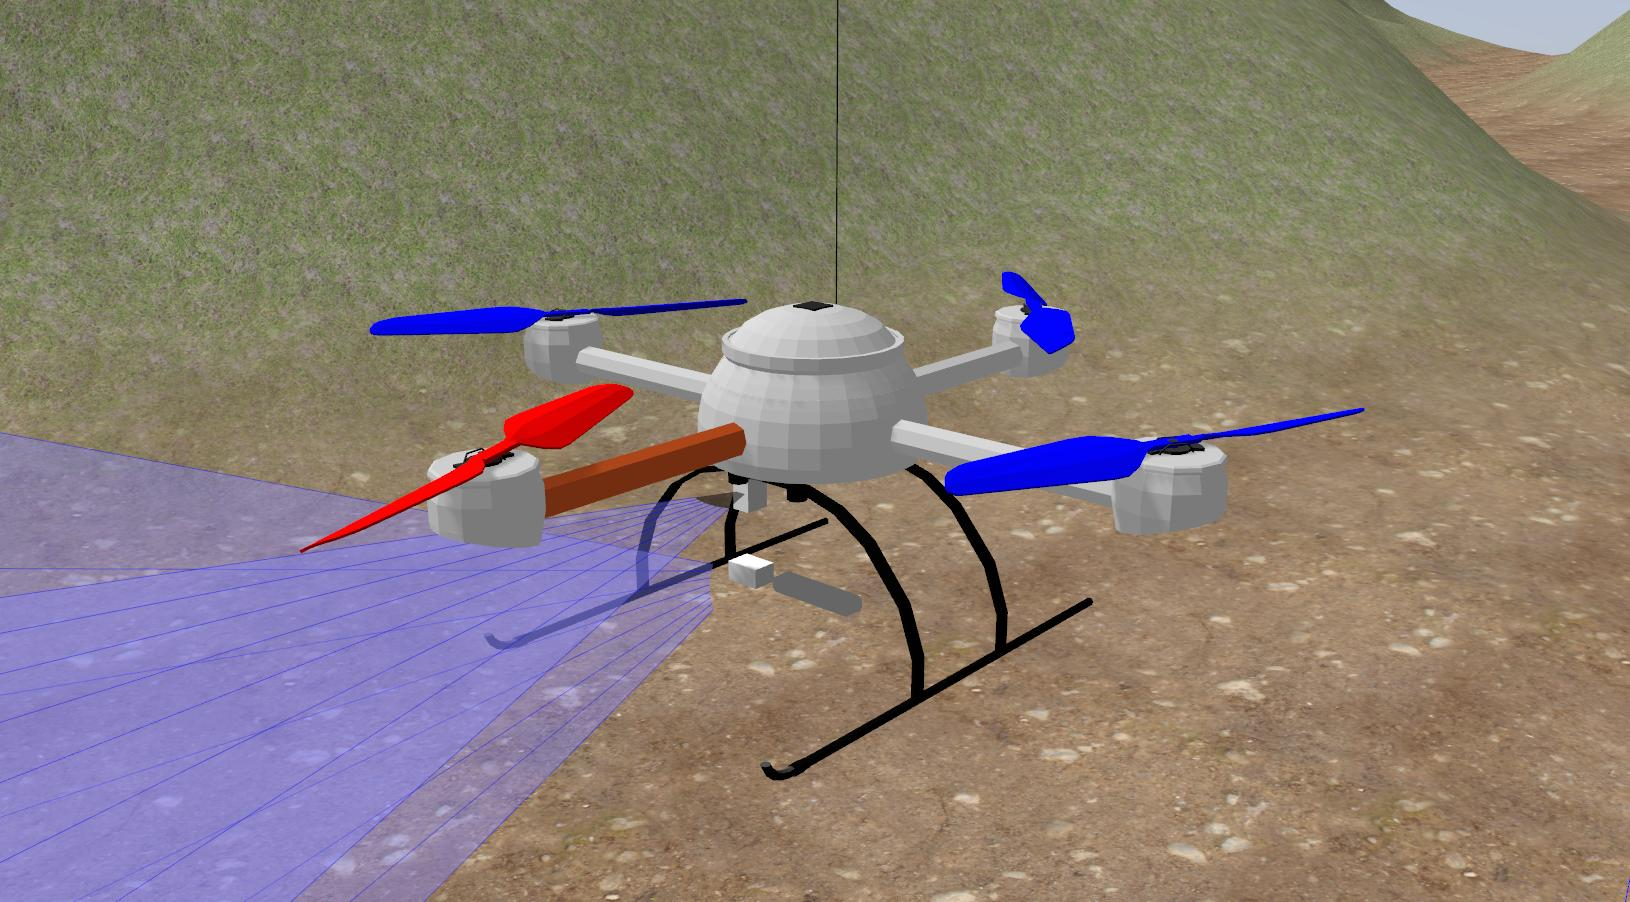
\includegraphics[width=0.7\linewidth]{images/sim_vehicle_closeup.jpg}
  \caption{Véhicule md4-1000 en simulation. Les rayons bleus sont les rayons projettés par les scanner lasers LeddarVu8.}
  \label{fig:sim_vehicle_closeup}
\end{figure}

Plusieurs environnements ont étés implémentés incluant un monde simulant un parc éolien avec plusieurs éoliennes alignées (Figure \ref{fig:sim_worlds} (B)) et un monde avec une seule éolienne avec une montage au loin (Figure \ref{fig:sim_worlds} (A)). La simulation suit le pire cas possible d'un parc éolien respectant les consignes du Département de l'Environnement du Royaume-Uni demandant un minimum de trois diamètres de rotor d'espacement entre chaque éolienne \citep{DOE2009}. Il faut noter que suite à des discussions avec des travailleurs de l'industrie, l'un des défauts de la simulation est que les pales des éoliennes sont normalement inclinées vers l'arrière de tel sorte qu'elles sont parallèles au sens du vent. Ceci permet au rotor de rester stationnaire lors des inspections.

\begin{figure}[htbp]
  \centering
  \begin{minipage}{0.49\textwidth}
    \centering
    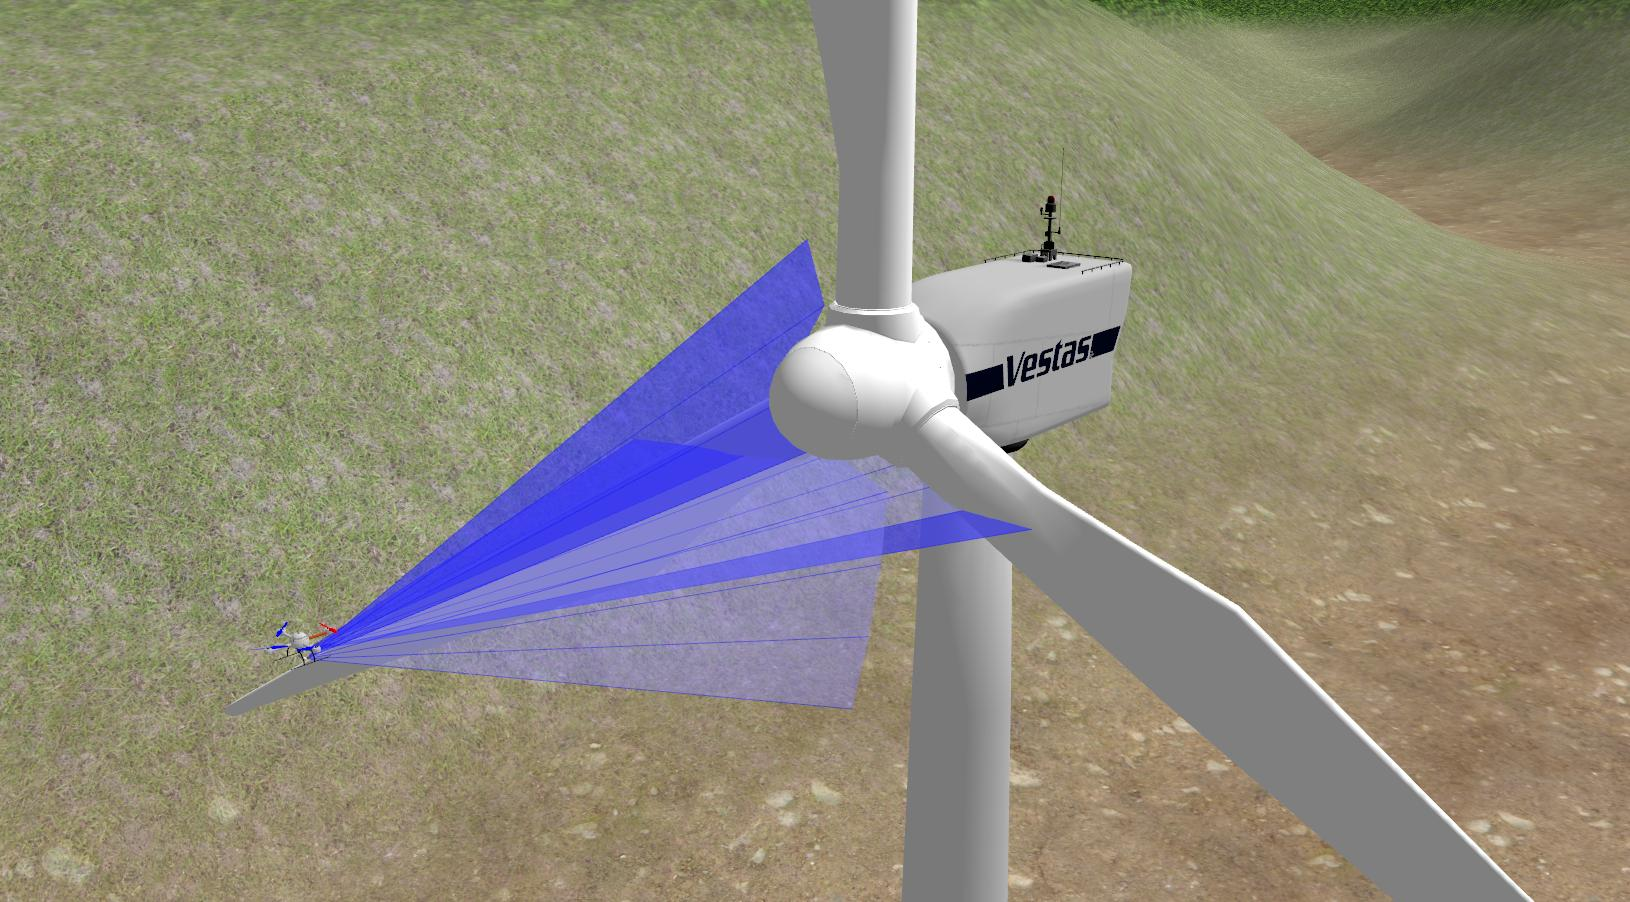
\includegraphics[width=\linewidth]{images/sim_vestas_closeup.jpg}
    (A)
  \end{minipage}
  \begin{minipage}{0.49\textwidth}
    \centering
    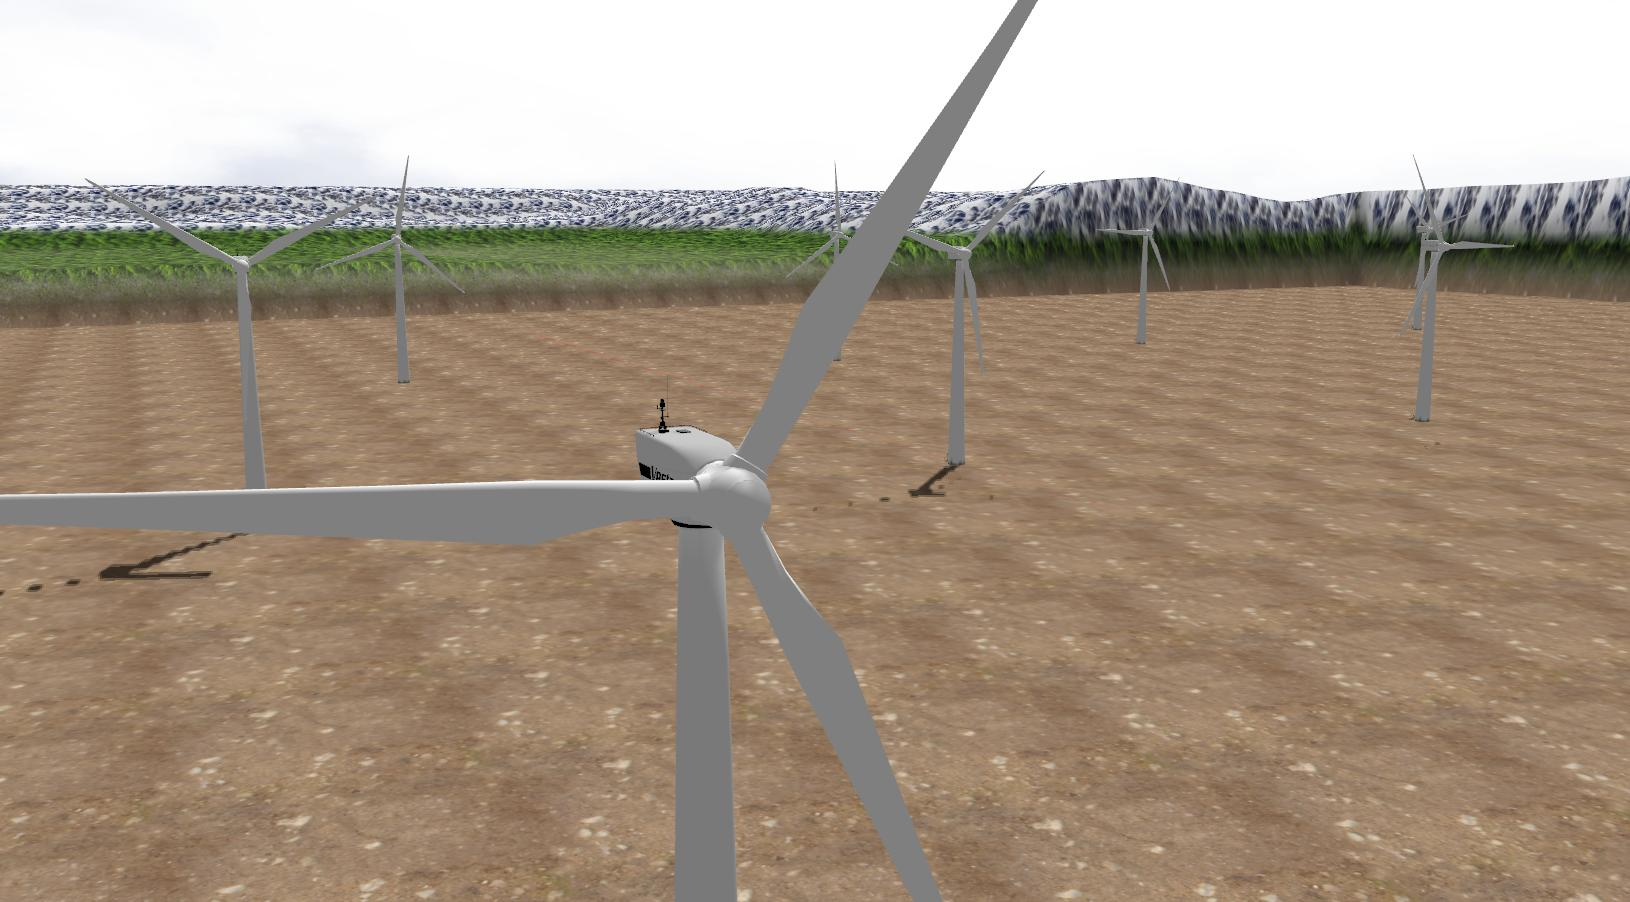
\includegraphics[width=\linewidth]{images/sim_vestas_multiple.jpg}
    (B)
  \end{minipage}
  \caption{Environnements de simulation.}
  \label{fig:sim_worlds}
\end{figure}

\subsubsection{Résultats par traitement d'images}

Tout d'abord nous testons en simulation la méthode de Stokkeland modifiée. Nous pouvons observer dans la Figure \ref{fig:sim_detection} (A) une détection réussie en présence d'un angle de roulis et dans la Figure \ref{fig:sim_detection} (B) une détection lorsque l'horizon est présent près du rotor. Le grand cercle vert représente le rayon de recherche autour du quel les segments de pale sont recherchés, les petits cercles verts sont les intersections des projections des pales, le cercle rouge est la moyenne des intersections (le centre du rotor) et le cercle rose est la sortie du filtre de Kalman.
\begin{figure}[htbp]
  \centering
  \begin{minipage}{0.49\textwidth}
    \centering
    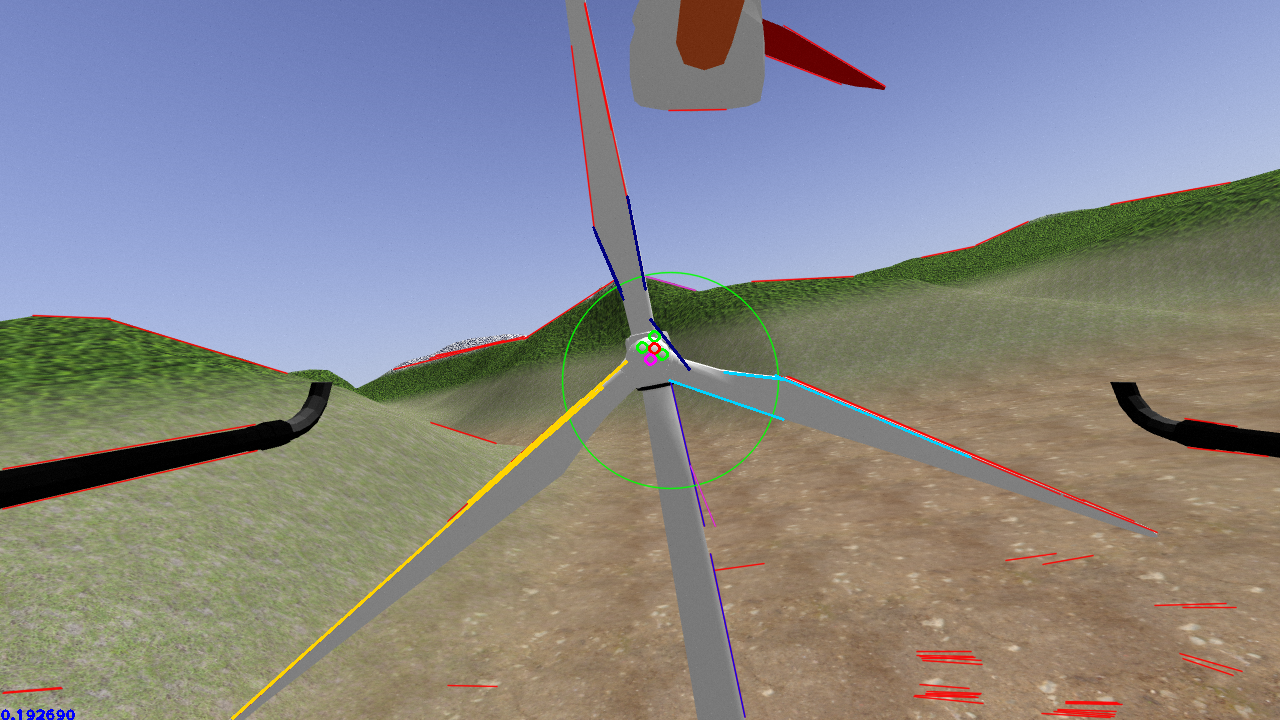
\includegraphics[width=\linewidth]{images/sim_detection.png} (A)
  \end{minipage}
  \begin{minipage}{0.49\textwidth}
    \centering
    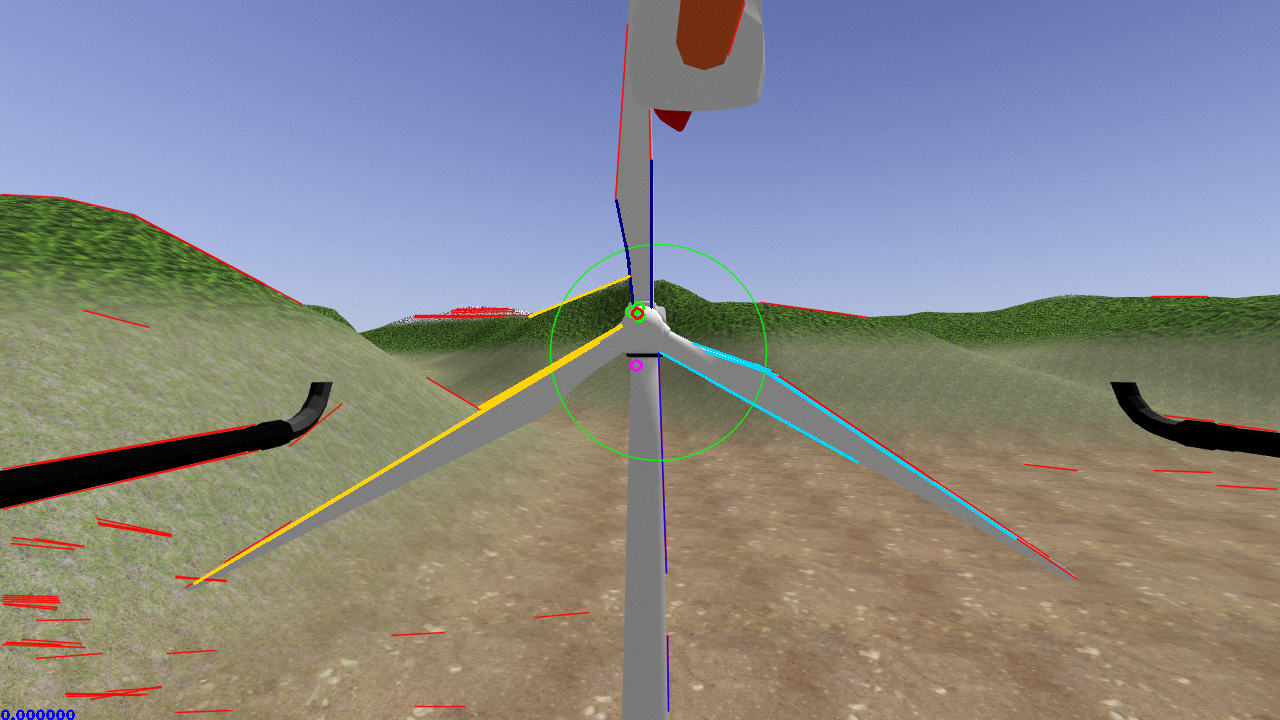
\includegraphics[width=\linewidth]{images/sim_detection3.png} (B)
  \end{minipage}
  \caption{Détections réussies en simulation.}
  \label{fig:sim_detection}
\end{figure}

Suite à beaucoup d'expérimentation, il devient difficile d'apprécier cette méthode et nous démontrons qu'une approche entièrement visuelle sans information au préalable n'est pas pratique. Dans nos tests en simulant une trajectoire d'avance manuellement à l'aide d'une manette, le taux de détection varie grandement entre 10\% et 60\% et dépend fortement du réglage des divers paramètres au niveau des filtres Gaussiens, de la détection des contours et des lignes et des divers paramètres de distance de recherche. De plus, une fois les paramètres règlés pour augmenter le taux de détection, ceux-cis deviennent invalides lorsque l'on modifie les paramètres de l'environnement de simulation tel que l'angle des pales, la texture du sol, les nuages dans le ciel et la position de la source de lumière. Un autre des problèmes rencontrées est la difficulté de choisir les paramètres du flou Gaussien tel que la texture de l'arrière plan est atténué tout en préservant les contours de l'éolienne pour l'algorithme de Canny. En somme, il est impossible de règler les paramètres au préalable pour accomoder toutes les conditions possibles qui seront rencontrés sur le terrain.

Nous profitons de la présence de la caméra stereo ZED simulée pour tester le fonctionnement de la résolution de la profondeur sur la surface de l'éolienne. Nous pouvons observer dans la Figure \ref{fig:stereo_fail} que la surface blanche de l'éolienne ne comporte pas assez de texture pour bien calculer la résolution de blocs. Résultat innatendu, le calcul de profondeur fonctionne parfois près de la bordure de l'objet où la transition entre la pale blanche et l'arrière plan donne une caractéristique pouvant être mis en correspondance dans l'image de droite. Par contre, lorsque la pale est horizontale, elle devient quasi-invisible du fait que la bordure est parallèle à la géométrie épipolaire. Ce problème est bien connu par les chercheurs utilisant la vision stéréoscopique pour le calcul de profondeur, certains tel que \citep{meier2017real} ont récemment proposé une solution possible à l'aide de caméras stereo orthogonales, cependant la résolution de ce problème sort du cadre de ce projet.

\begin{figure}[htb]
  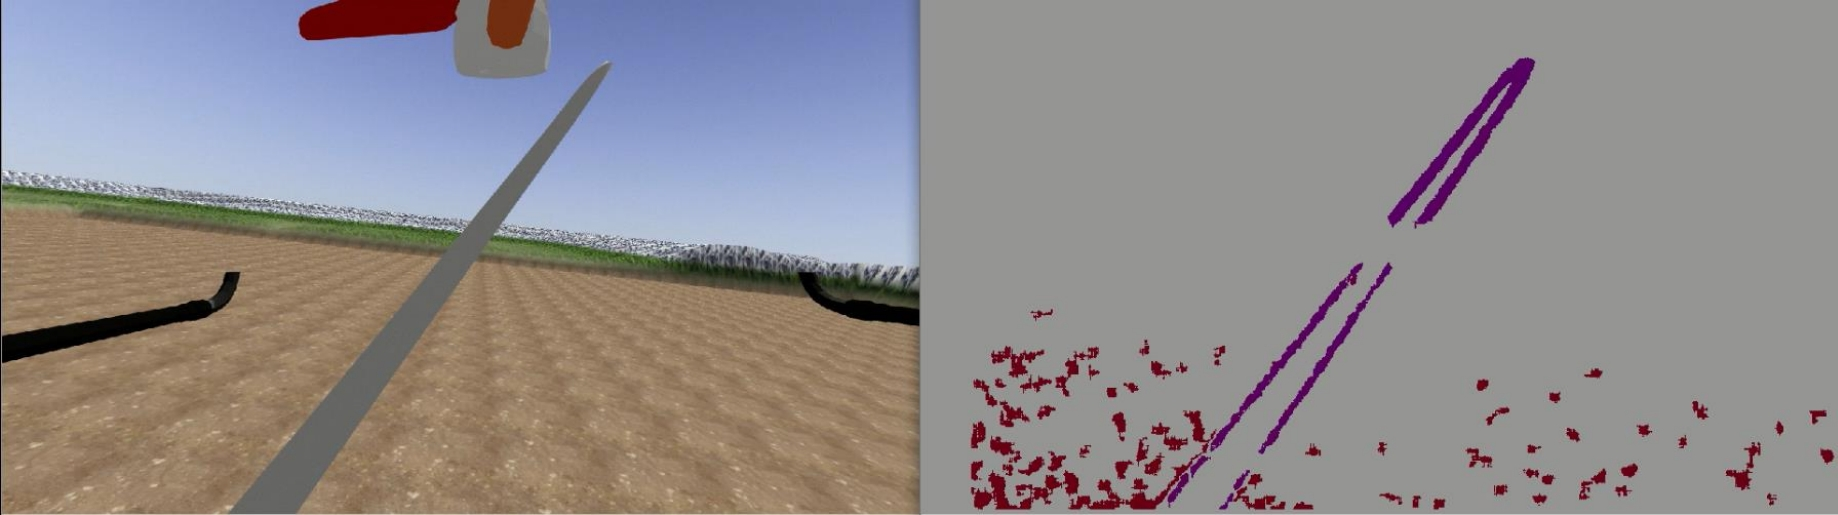
\includegraphics[width=\linewidth]{images/stereo_failure.jpg}
  \caption{Échec de la résolution de profondeur par correspondance de blocs.}
  \label{fig:stereo_fail}
\end{figure}

\subsubsection{Résultats du suivit par laser}

La mission d'inspection entièrement par laser se déroule avec succès dans une grande variété de scénarios. Dans cette section nous présentons et analysons l'un des vols effectués sur une éolienne avec pour seule information \textit{a priori} que l'une des pales a été placée vers le haut. Dans la Figure \ref{fig:sim_tower_total} on peut observer la trajectoire entière exécutée par l'UAV avec les différentes phases séparées par couleur. Outre une petite discontinuité dans la trajectoire de la pale 3, la majorité du vol s'exécute de façon lisse.
\begin{figure}[!htb]
  \centering
  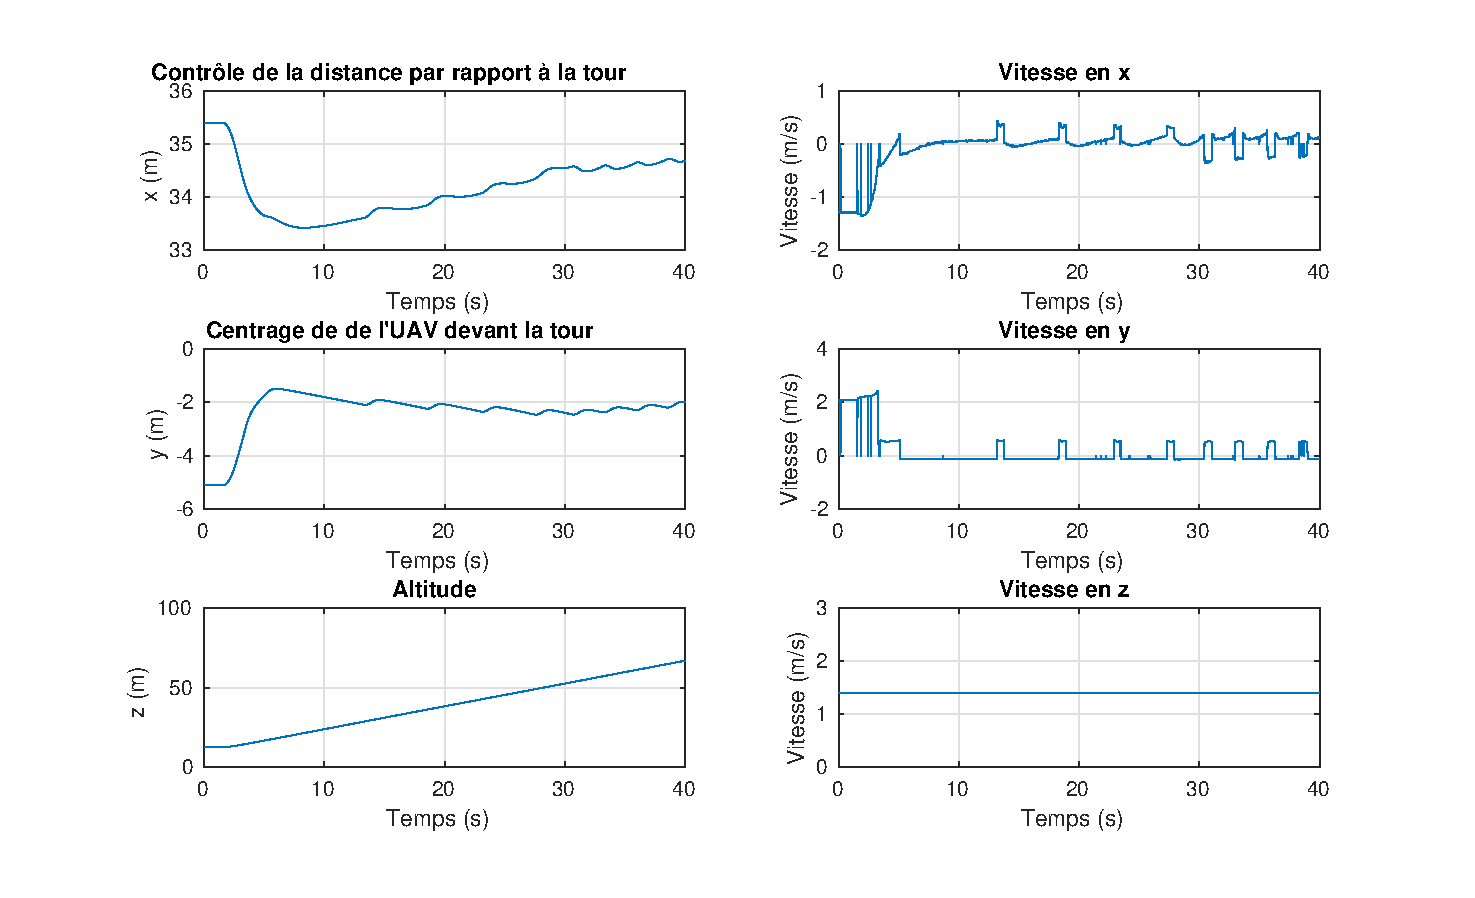
\includegraphics[width=\linewidth]{images/sim_tower_ascent}
  \caption{Trajectoire suivie pour la montée de la tour.}
  \label{fig:sim_tower_ascent}
\end{figure}

Dans la Figure \ref{fig:sim_tower_ascent} nous pouvons voir la décomposition de la trajectoire suivie pour monter la tour. L'UAV commence légèrement décentré par rapport à la tour et tente immédiatement de se centrer. La vitesse commandée en $z$ est constante et on voit que l'altitude augmente de façon lisse. Par contre on peut voir que la trajectoire en $x$ et en $y$ est légèrement saccadée. En $x$ la raison est une combinaison de gains PID légèrements trop aggressifs et du fait que le diamètre de la tour change au fur et à mesure qu'elle monte. En $y$ le problème provient plutôt de la faible résolution du scanner laser. Avec seulement 8 points, la bordure de la tour se retrouve entre deux rayons du laser, les différentes bosses dans la courbe $vy$ sont les instants où l'un des rayons adjacent au centre frappe la tour. À cet instant le terme d'erreur devient non nul et le robot bouge latéralement.
\begin{figure}[htb]
  \centering
  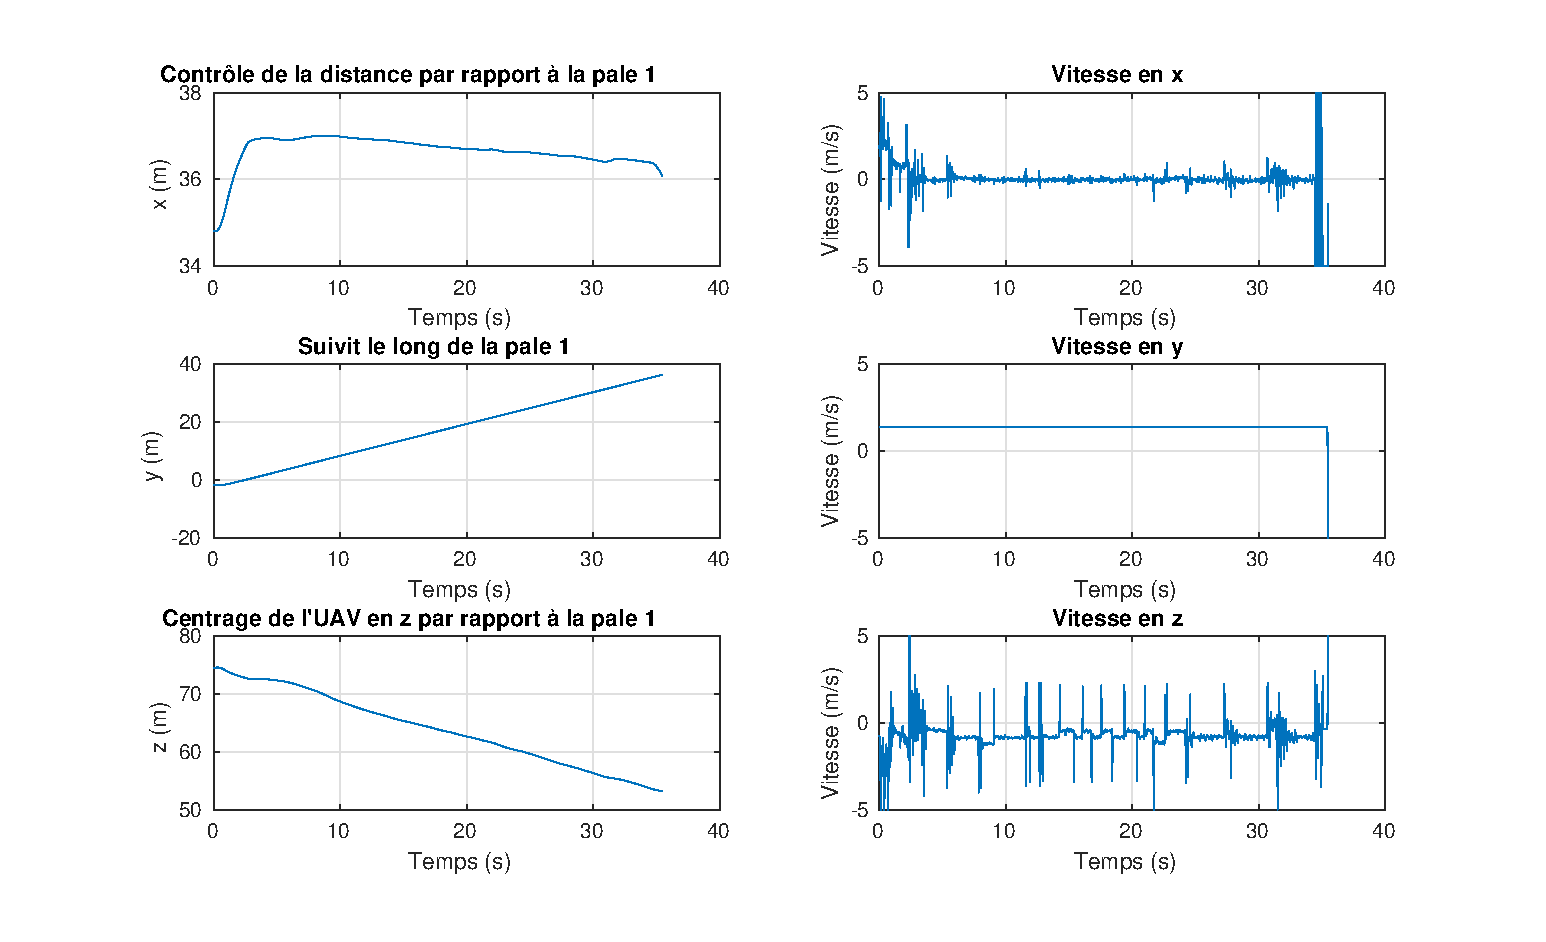
\includegraphics[trim=30 20 30 0, clip, width=\linewidth]{images/sim_suivit_pale}
  \caption{Trajectoire pour le suivit de la pale 1.}
  \label{fig:sim_suivit_pale}
\end{figure}

La Figure \ref{fig:sim_suivit_pale} présente la trajectoire et les commandes de vitesses pour le suivit de la pale 1. Nous voyons que les vitesses en $z$ semblent saccadées mais ceci est encore dût au petit nombre de rayons du scanner laser. Chaque petit pic est en fait un instant où un rayon supplémentaire du laser parvient à toucher la surface de la pale et influencer le calcul de son centre. Vers la fin de la courbe $vx$ nous pouvons observer une oscillation entre la commande $0$, $+5$ et $-5$ mètres par secondes. Ceci est dû au fait que la fin de la pale est assez petite pour passer entre deux rayons du scanner laser, combiné au mouvement de tangage du véhicule pour avancer et reculer le laser parvient momentanément à toucher la pale. En réalité ceci ne devrait pas être un problème car le LeddarVu8 ne souffre pas des angles morts entre ses rayons. Malgré cela, le robot poursuit son chemin jusquà ce que la fin de la pale soit officiellement détecté par le compteur de lectures vides.
\begin{figure}[htb]
  \centering
  \includegraphics[trim=30 10 10 50,clip,width=0.5\linewidth]{images/sim_tower_total}
  \caption{Trajectoire complète d'inspection.}
  \label{fig:sim_tower_total}
\end{figure}

\clearpage
\subsection{Résultats de tests sur le terrain}
\label{subsec:results_field}

\begin{figure}[htb]
  \centering
  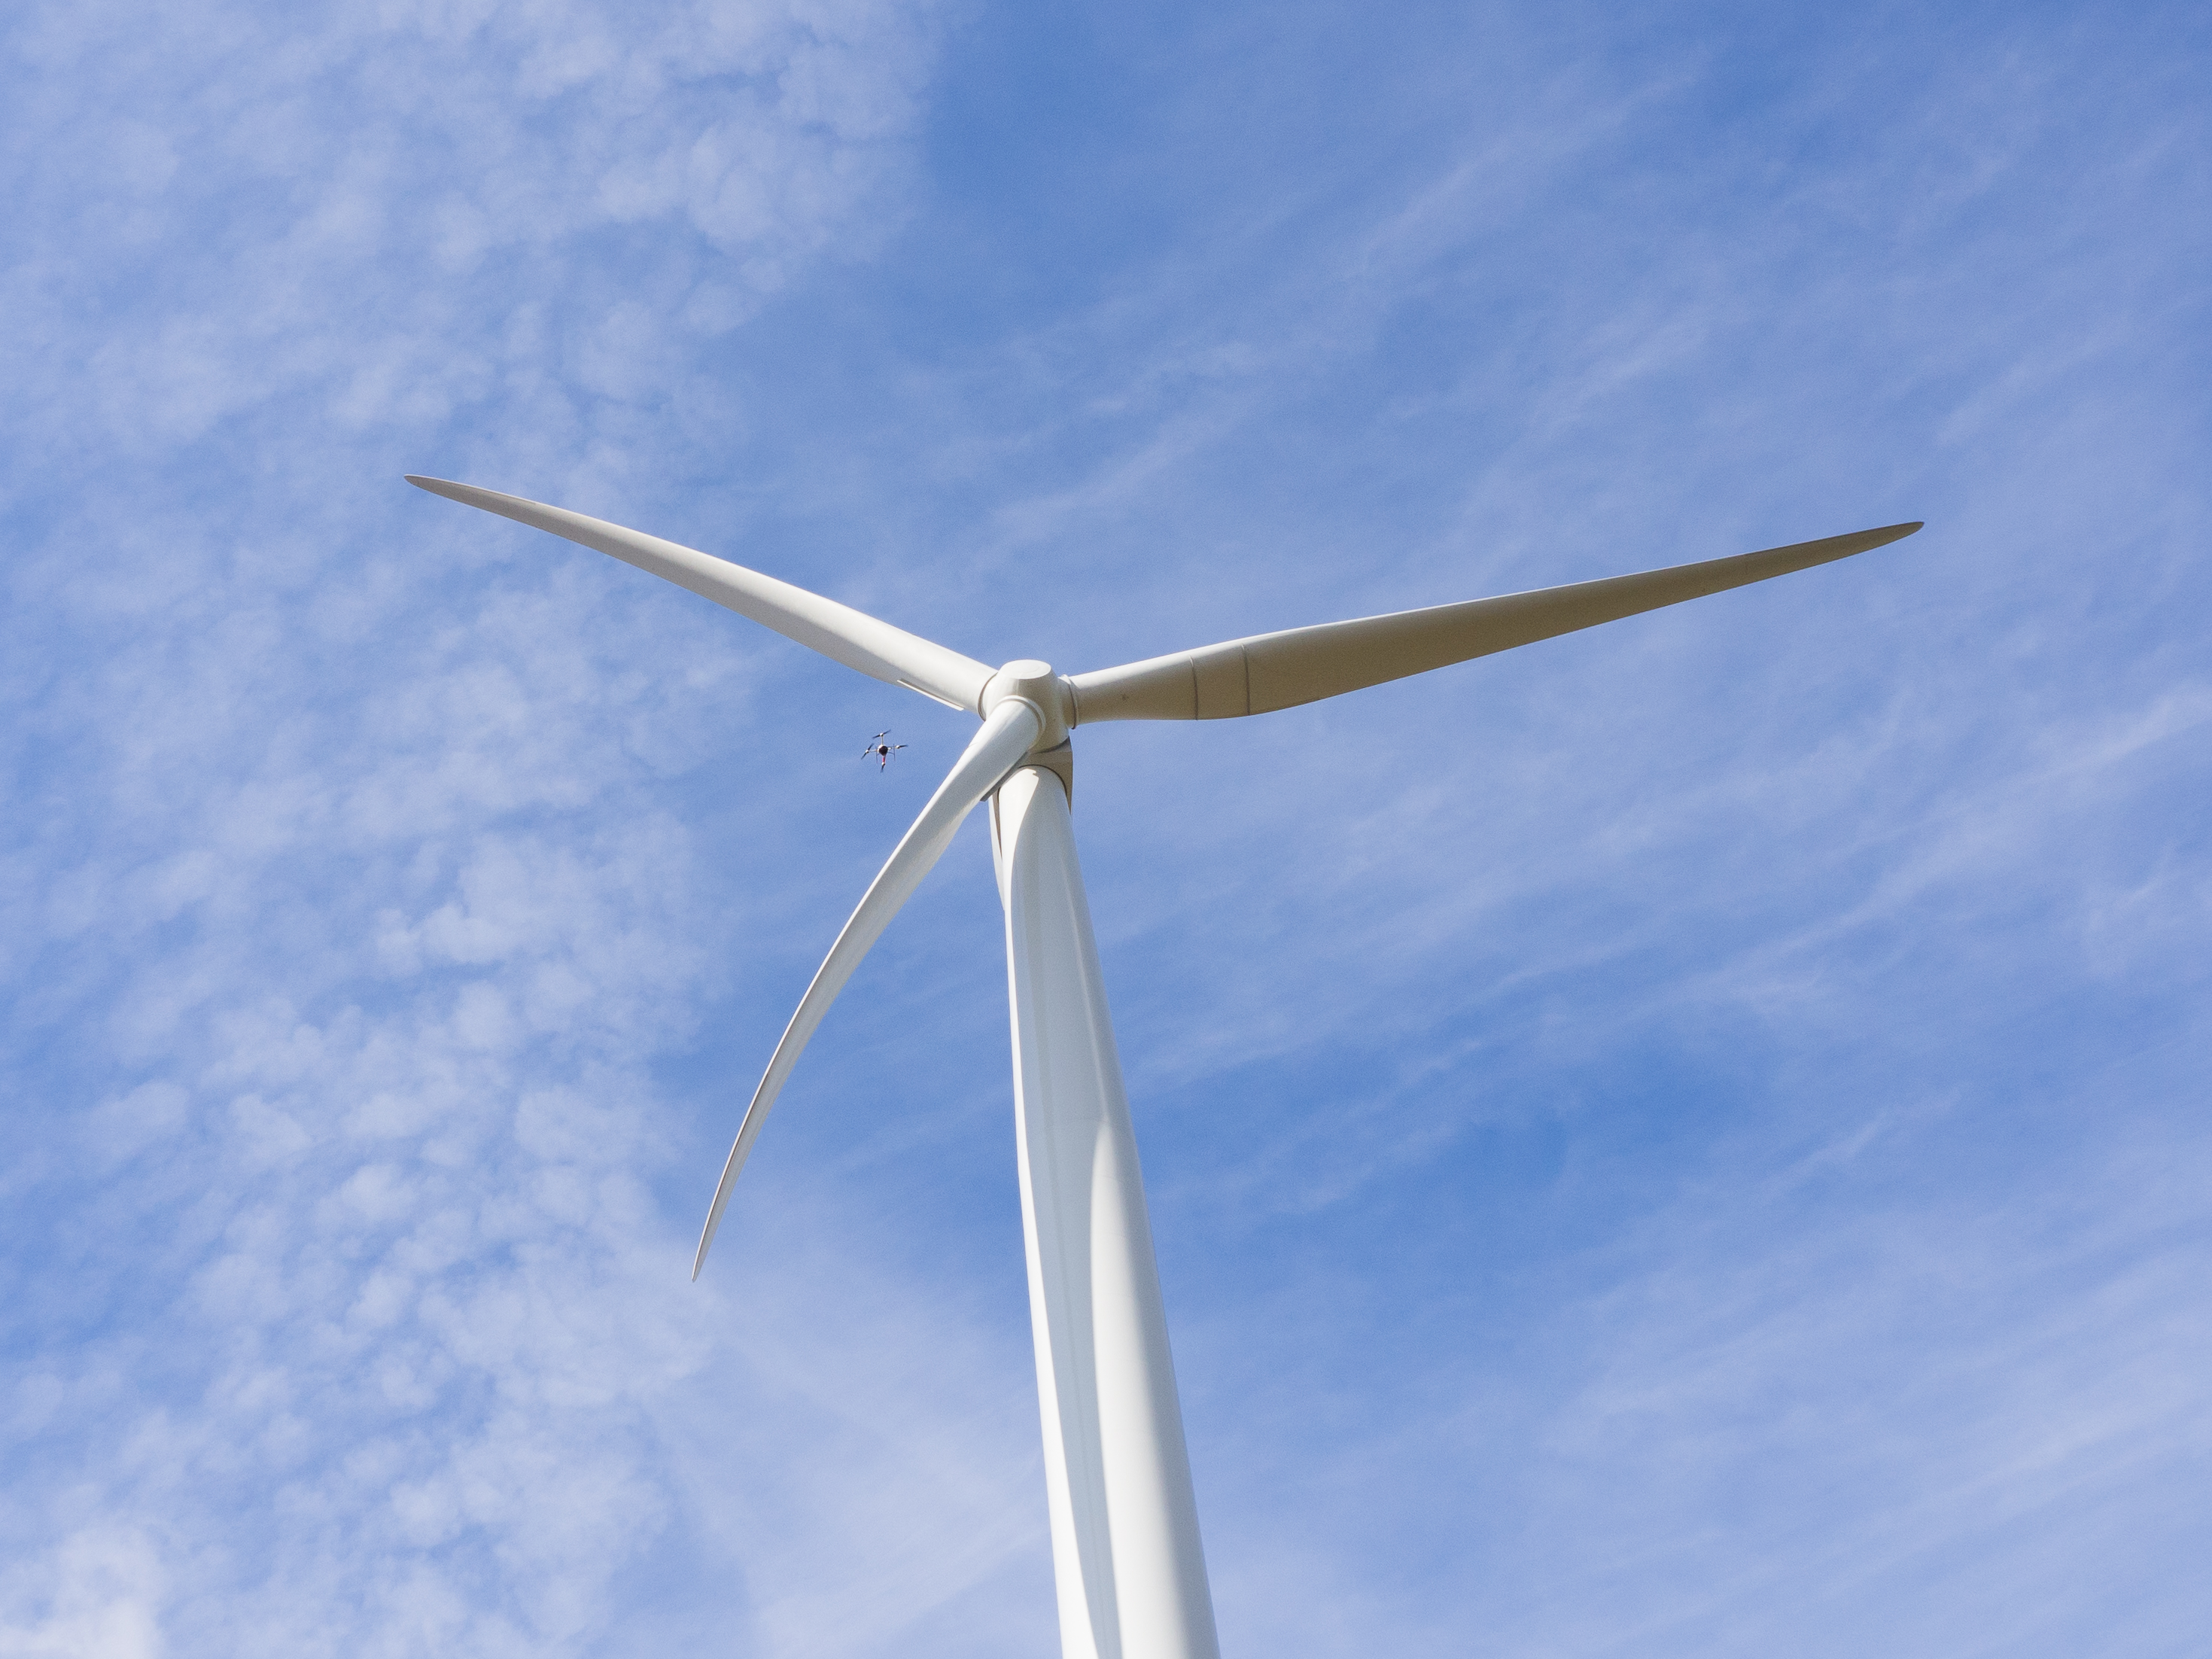
\includegraphics[trim=180 200 180 180,clip,width=\linewidth]{images/test_eolienne.jpg}
  \caption{Le md4-1000 en vol inspectant l'une des pales.}
  \label{fig:test_eolienne}
\end{figure}

Suivant les spécifications initiales, l'intégration des capteurs s'est faite sur un md4-1000 pris en photo dans la Figure \ref{fig:field_vehicle} pour faire un test de vol manuel nous permettant de confirmer certaines de nos hypothèses au niveau de la vision stereo. Le système d'exploitation Ubuntu 16.04 a été installé sur l'ordinateur Nvidia TX2 avec des modifications apportées au noyau Linux fourni par Nvidia à fin de permettre au TX2 d'interfacer avec les différents périphériques à bord de la planche de support AuvIdea J140. Les LeddarVu8 et la caméra ZED sont branchés par USB3 alors que la communication au md4-1000 se fait par UART.

\begin{figure}[htp]
  \centering
  \begin{minipage}{0.45\textwidth}
    \centering
    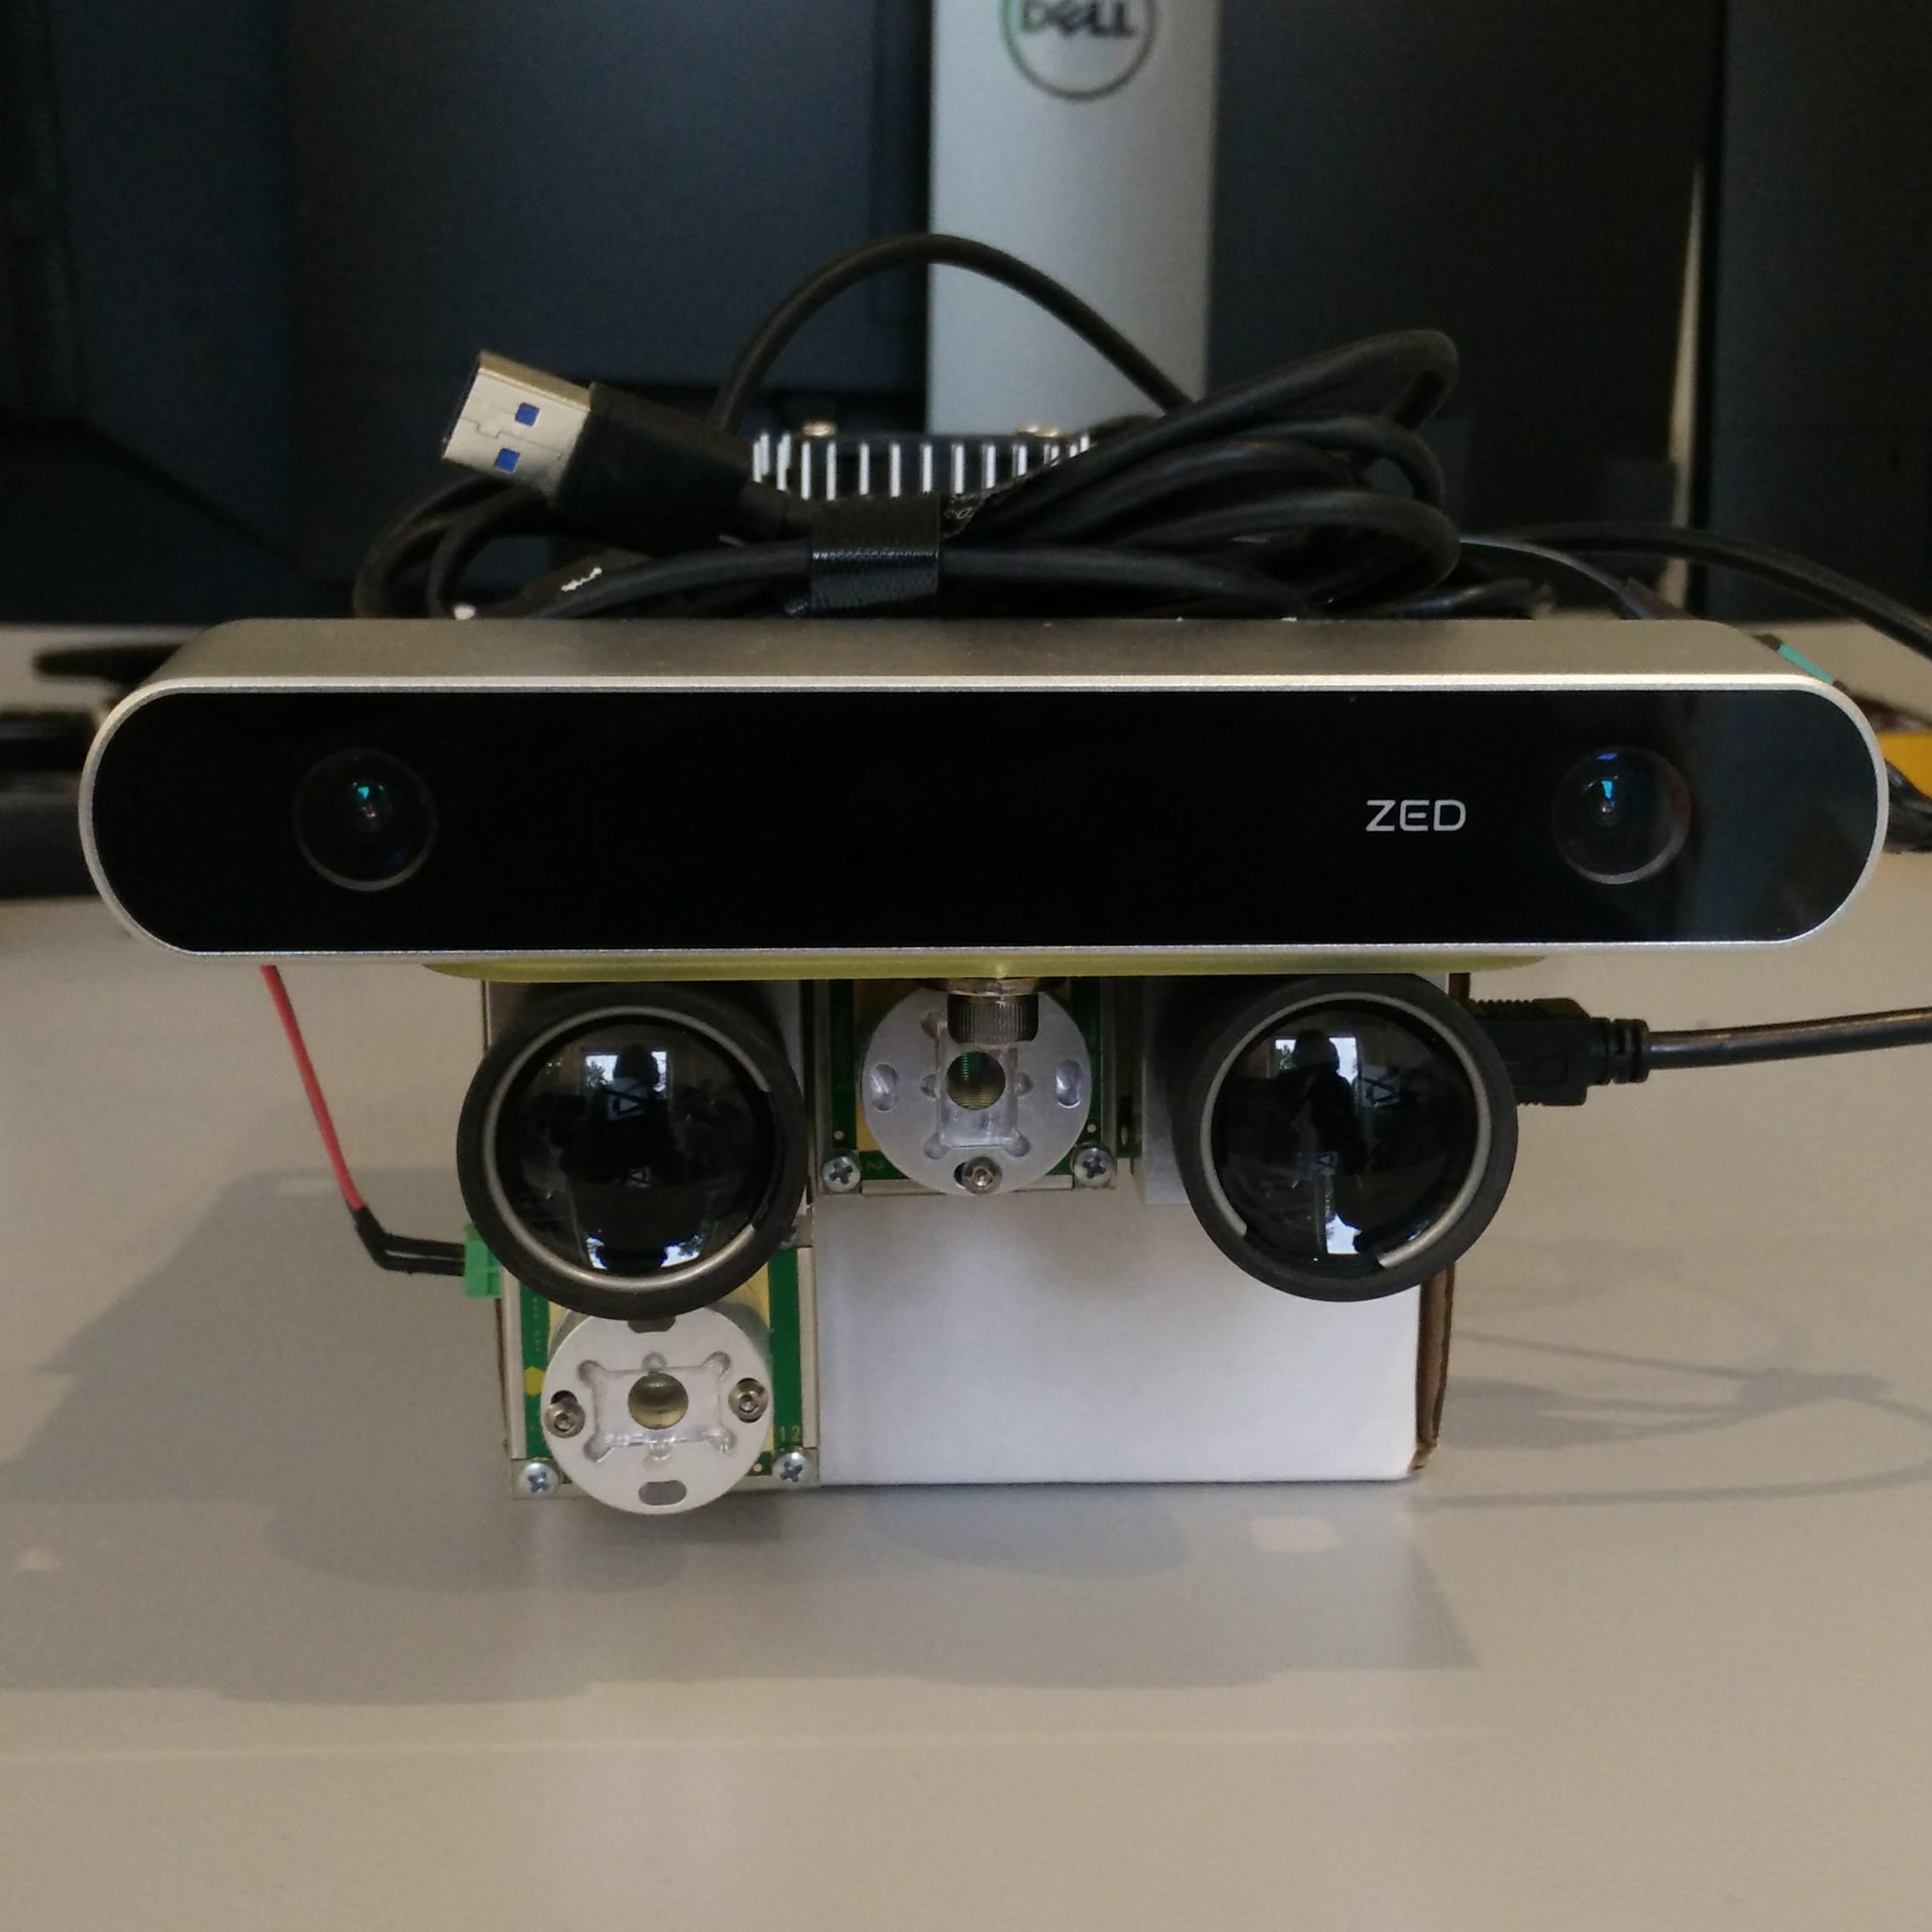
\includegraphics[width=\linewidth]{images/payload.jpg}
    (A)
  \end{minipage}
  \begin{minipage}{0.45\textwidth}
    \centering
    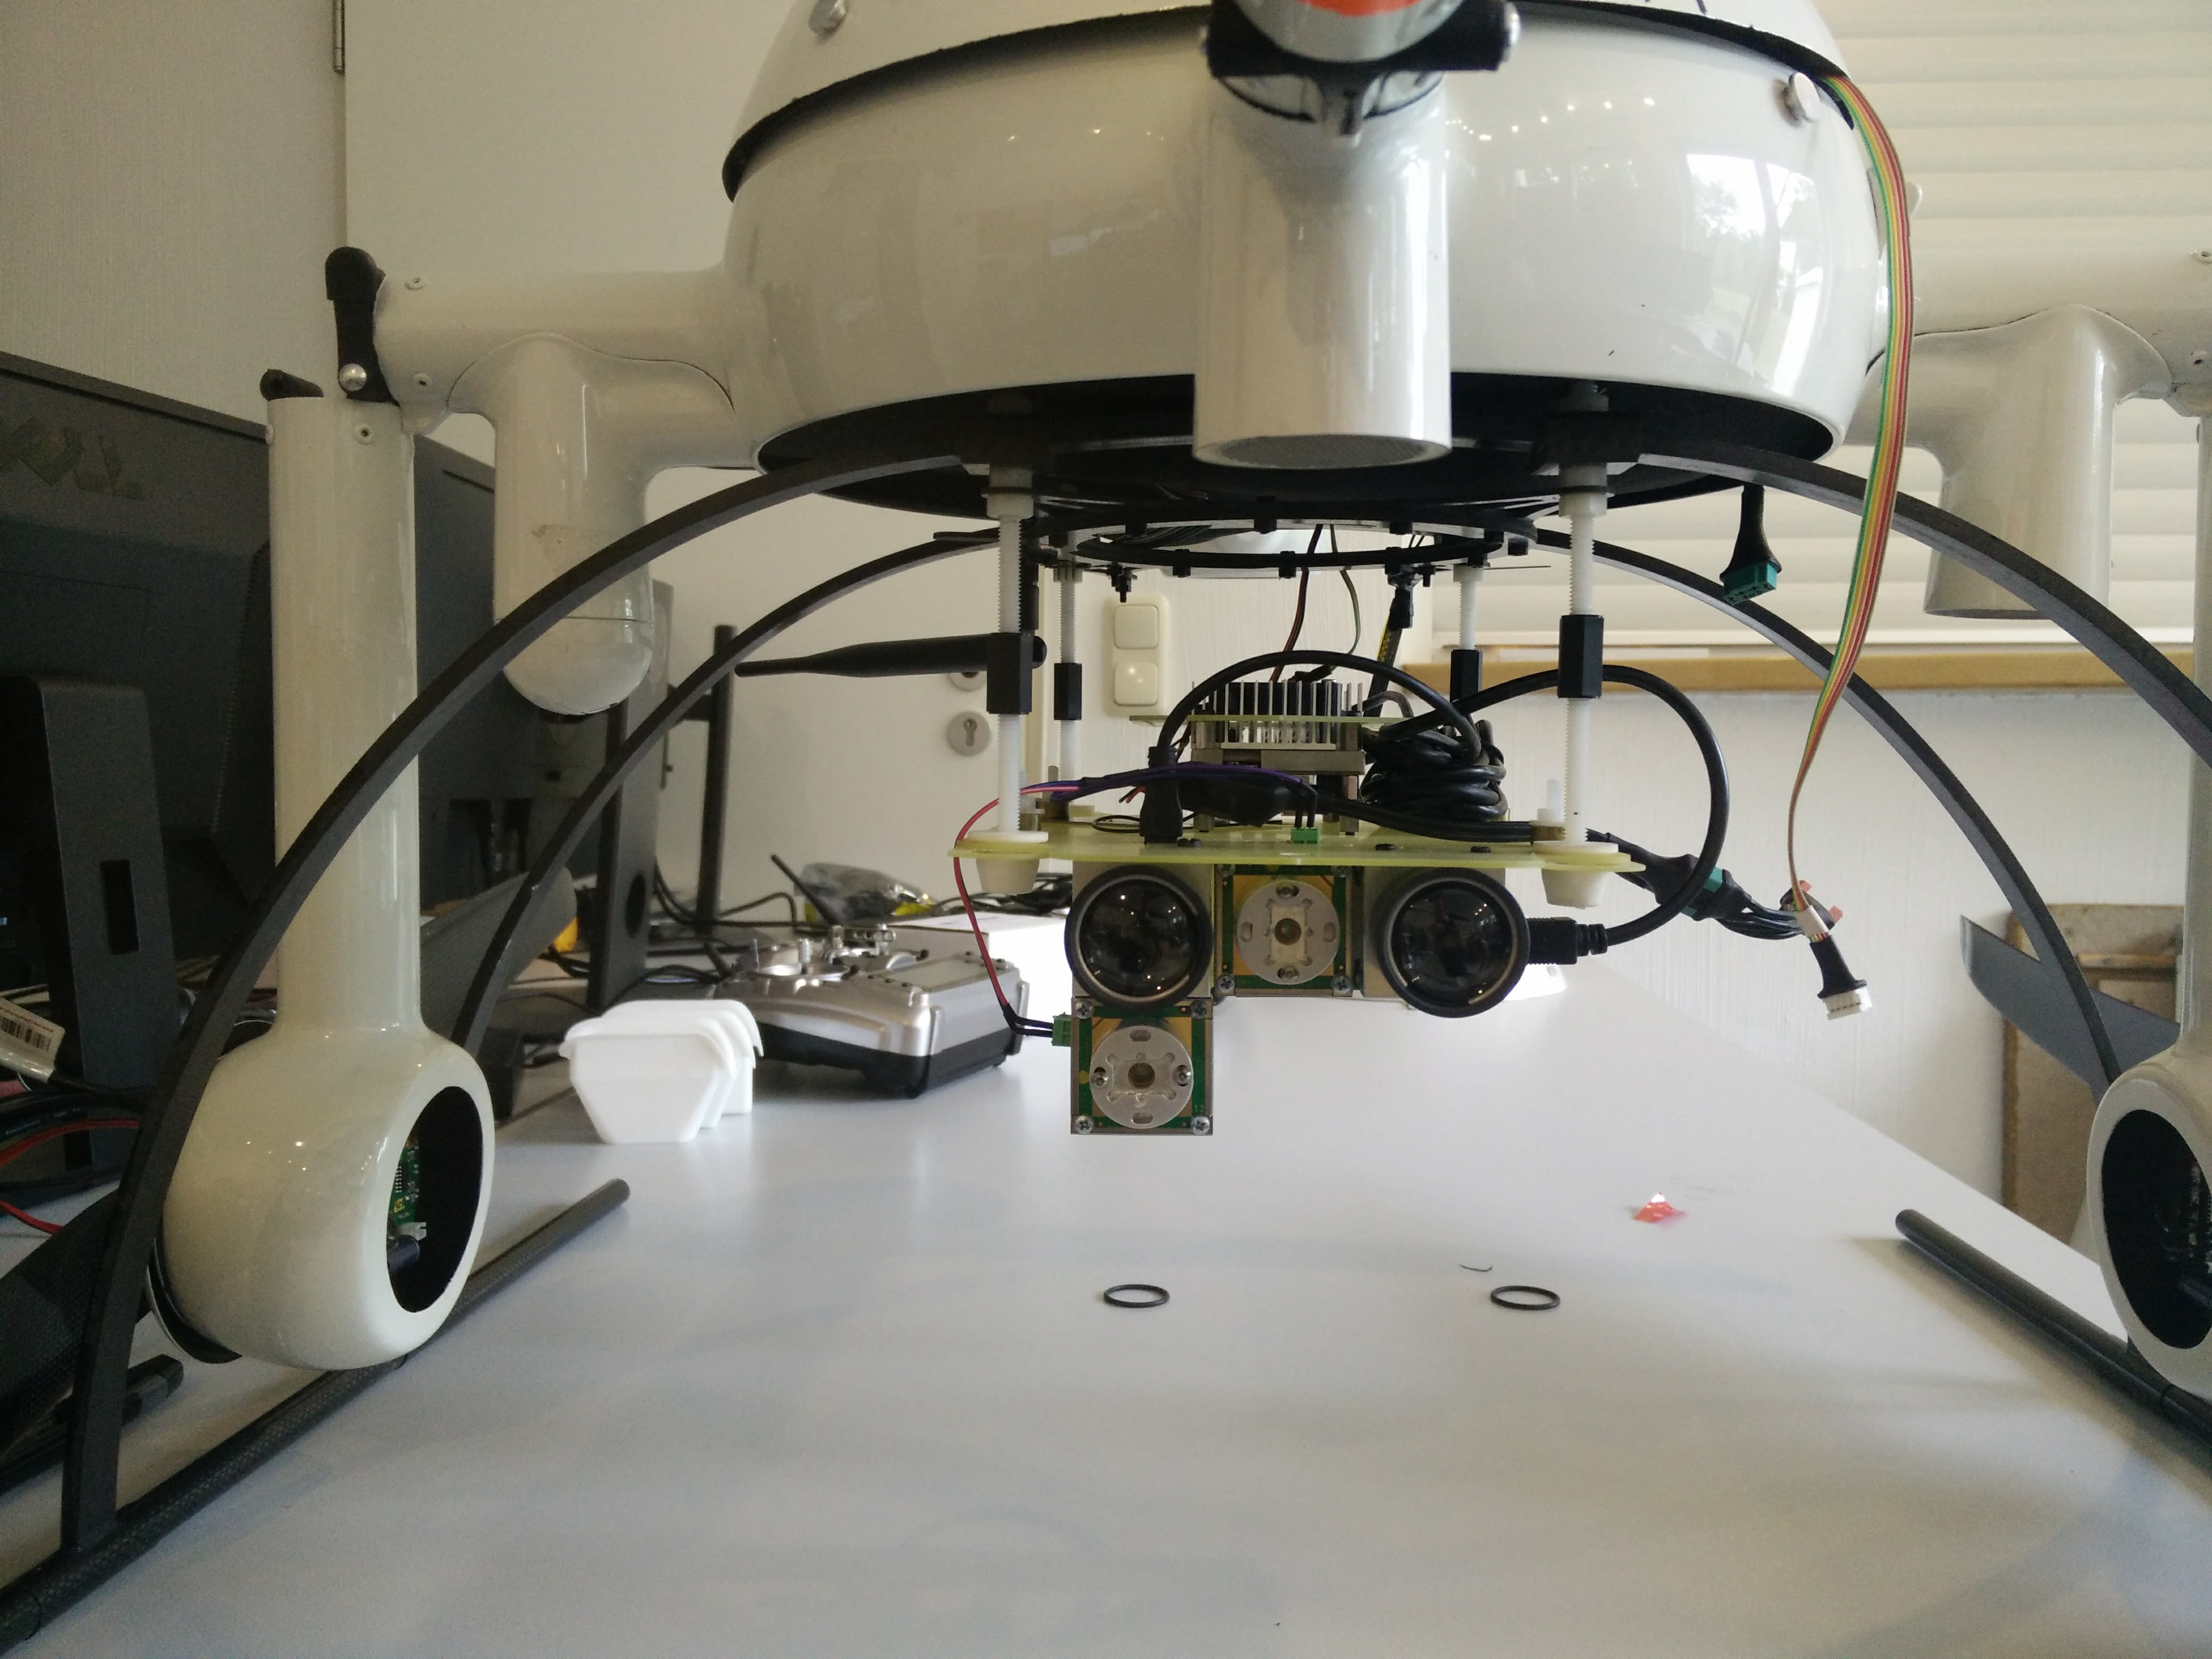
\includegraphics[width=\linewidth]{images/payload2.jpg}
    (B)
  \end{minipage}
  \caption{Véhicule md4-1000 avec les capteurs et l'ordinateur de bord intégré. (A) Caméra ZED et les télémètres lasers LeddarVu8. (B) La charge utile installé sur le robot (sans la ZED), avec la Nvidia TX2 visible.}
  \label{fig:field_vehicle}
\end{figure}

Les tests de vol ont été effectués au parc éolien Pierre-de-Saurel où la hauteur de la tour est de $100$ mètres et le diamètre du rotor est de $92.5$ mètres. La Figure \ref{fig:test_eolienne} nous donne un ordre de grandeur de la structure par rapport à l'UAV.

% En collaboration avec le personnel de Microdrones, une procédure d'inspection a été développée pour assurer une mission sécuritaire.
%
% \begin{enumerate}
%   \item La nacelle est tournée en aval du vent, c'est-à-dire que le vent arrive de l'arrière de l'éolienne. Ceci a pour effet que si jamais le signal GPS est perdu ou que l'interférence magnétique cause une perte du contrôle de position, l'UAV s'éloignera de la structure.
%   \item Les pales sont tournées parallèles au vent pour les empêcher de tourner.
%   \item Un système de télémétrie relai au pilote la distance moyenne des objets détectés par les lasers.
%   \item Un observateur se place près de la tour pour prévenir le pilote de dangers de collision.
% \end{enumerate}

La caméra stereo s'avère à avoir une performance extrêmement variable à travers le vol tel que l'on peut voir dans la Figure \ref{fig:field_stereo_fail}. Il est difficile de corréler exactement les charactéristiques de la scène au succès ou à l'échec de la résolution de profondeur. Dans certains cas une pale diagonale est invisible alors que dans le dernier exemple elle est parfaitement visible. On voit aussi que le ciel clair est parfois résolu par erreur. Par conséquent, nous prouvons notre hypothèse initiale et en concluons qu'une caméra stereo est inutilisable dans le contexte de l'inspection d'éoliennes.

\begin{figure}
  \begin{tabular}{cc}
    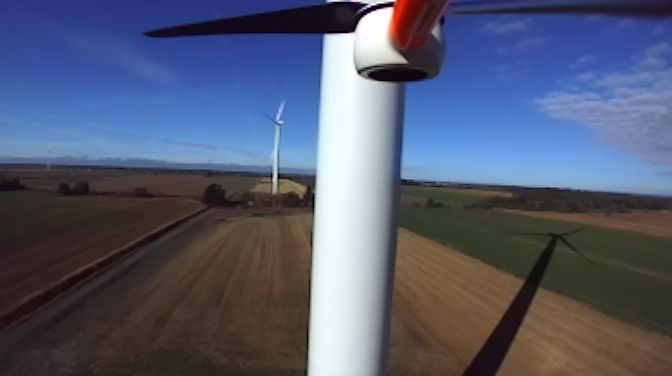
\includegraphics[width=0.5\linewidth]{images/field_stereo_fail_rgb.png} &
    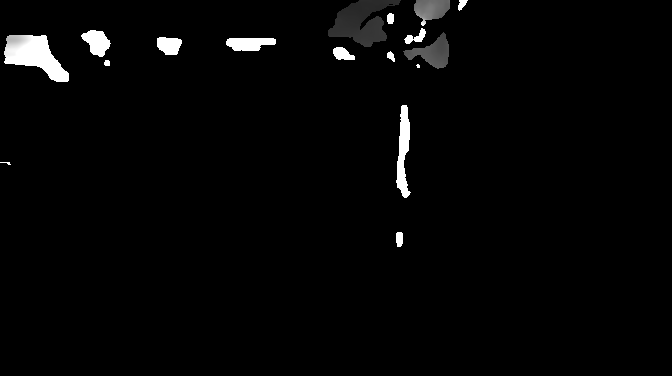
\includegraphics[width=0.5\linewidth]{images/field_stereo_fail_pcl.png} \\
    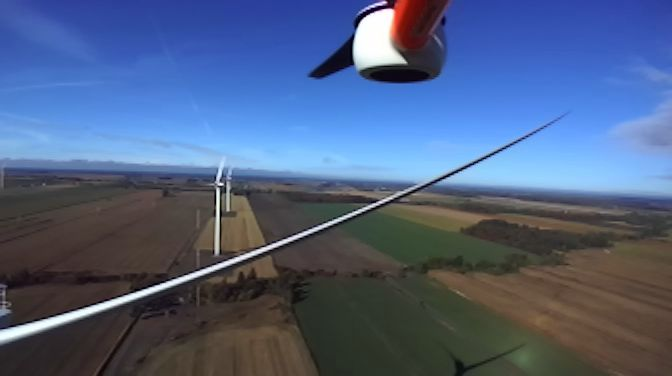
\includegraphics[width=0.5\linewidth]{images/field_stereo_fail_rgb2.png} &
    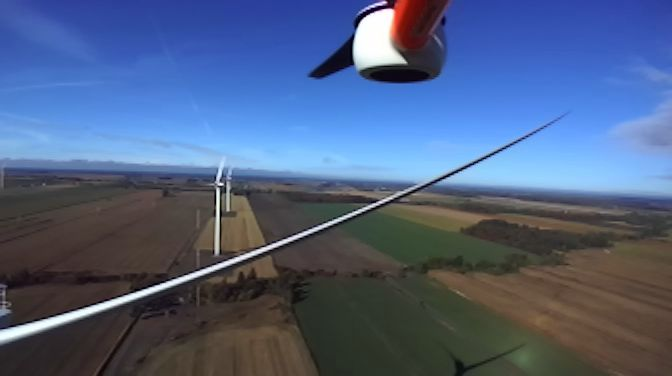
\includegraphics[width=0.5\linewidth]{images/field_stereo_fail_rgb2.png} \\
    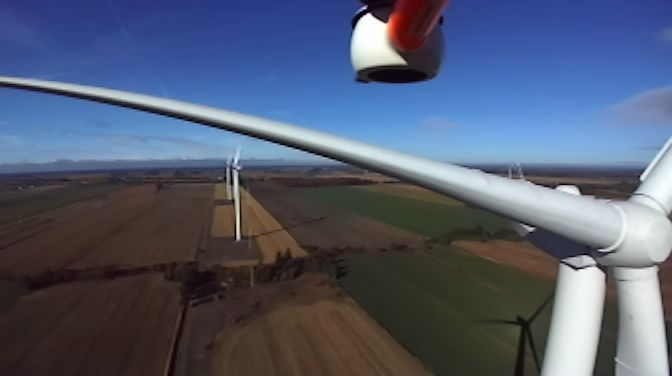
\includegraphics[width=0.5\linewidth]{images/field_stereo_success_rgb.png} &
    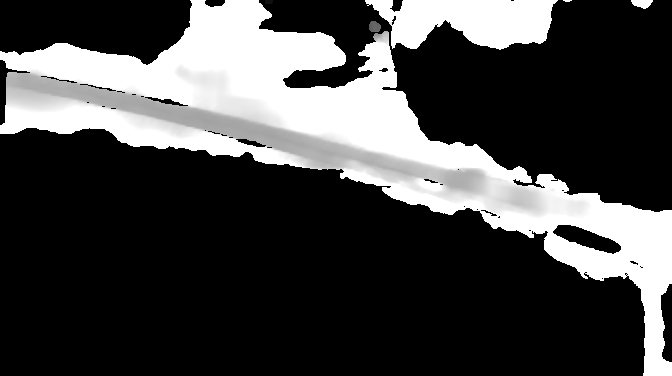
\includegraphics[width=0.5\linewidth]{images/field_stereo_success_pcl.png} \\
    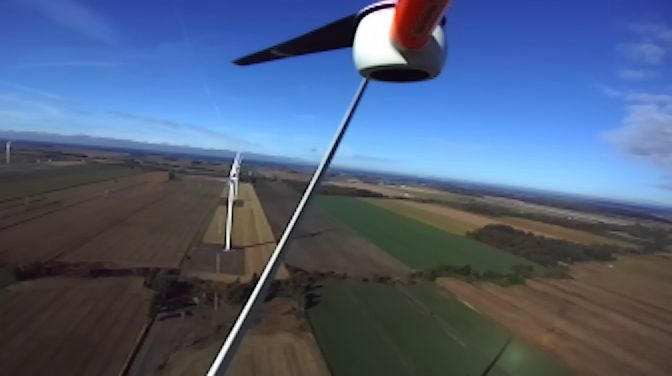
\includegraphics[width=0.5\linewidth]{images/field_stereo_success_rgb2.png} &
    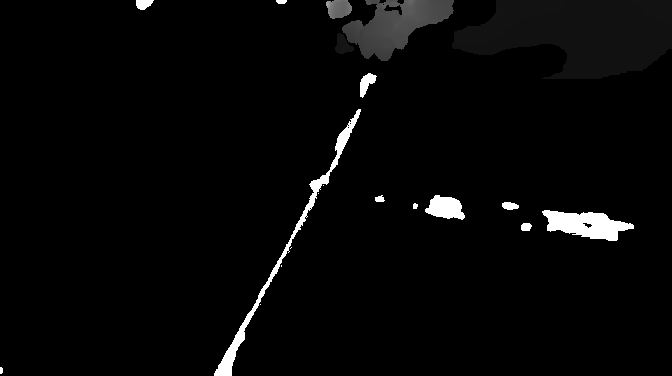
\includegraphics[width=0.5\linewidth]{images/field_stereo_success_pcl2.png} \\
  \end{tabular}
  \caption{Exemples de succès et d'échecs de perception de distance. À gauche les images RGB de la caméra de gauche et à droite les images de profondeur ramenées sur la caméra de gauche.}
  \label{fig:field_stereo_fail}
\end{figure}

\color{red}
En ce qui concerne l'approche par laser il n'a pas été possible de tester le système sur le terrain en raison de différentes circonstances (ils ont pas mit le frein alors l'éolienne bougeait, le gars en allemagne a fait une erreure dans le driver du laser etc...). Plus de temps serait requis pour faire l'intégration et le réglage des gains PID sur le vrai véhicule. Par contre, puisque l'entièreté du logiciel est déjà écrit en C++ et prêt à installer sur le véhicule, il ne suffirait que de changer quelques branchements au niveau des flux de données pour faire les tests sur le terrain.
\color{black}

\clearpage
\section{Discussion des résultats et travaux futurs}

Bien que nous n'avons pas pu valider notre approche sur le terrain, les résultats en simulation demeurent prometteurs et l'inspection d'éoliennes reste un projet important à poursuivre dans le futur. Par contre, suite à nos tests de vol manuels sur le terrain nous réalisons maintenant que la méthode d'inspection bénificierait de plusieurs changements.

Tout d'abord, pour qu'un UAV entre $1$ et $25$ kg utilisé à des fins non-récréatives soit exempt du besoin d'un Certificat d'Opération Aériennes Spécialisées (COAS) par Transport Canada, il doit demeurer en dessous d'une altitude de $300$ pieds ($91$ mètres) \citep{transportscanada2016}. Puisque les grandes éoliennes ont leur nacelle à une altitude de $100$ mètres ou plus, ceci implique que chaque fois qu'un inspecteur voudrait aller travailler il faudrait appliquer pour un COAS à l'avance ce qui peut prendre beaucoup de temps à être approuvé. Sans quoi, l'UAV n'aurait pas le droit d'inspecter les pales autres que celles pointant vers le bas.

Il reste néanmoins une alternative possible qui comporterait plusieurs avantages sur le système proposé à condition de remettre en question les modalités de la participation de l'inspecteur et du budget alloué. Le système pourrait faire une inspection en 3 dimensions d'une seule pale à la fois pointée vers le bas suivant une trajectoire présenté dans la Figure \ref{fig:alternative}. En commençant sur le côté de la pale l'UAV longerait la pale vers bas. Il pivoterait ensuite pour remoter le bord d'attaque avant de pivoter une dernière fois pour longer le côté droit. Ceci demanderait des capteurs différents et que l'inspecteur fasse tourner les pales entre chaque vol mais aurait l'avantage d'avoir de bien meilleures images puisque la caméra serait pointée perpendiculairement à la surface à inspecter.

\begin{figure}[htb]
  \centering
  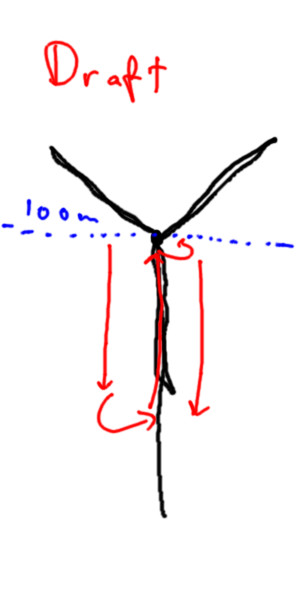
\includegraphics[width=0.3\linewidth]{images/cool_alternative.jpg}
  \caption{Trajectoire alternative pour l'inspection d'une pale à la fois sans besoin de COAS.}
  \label{fig:alternative}
\end{figure}

Pour en revenir à la méthode que nous proposons, l'UAV bénificierait grandement de l'utilisation de D-GPS ou de GPS-RTK à deux antennes. Le premier avantage serait que avec un positionnement plus précis il serait possible de se rapprocher beaucoup plus de la structure et obtenir de meilleures images. Les distances utilisées en simulation prennent en compte que la précision du positionnement du md4-100 est typiquement entre $\sigma = 1.0$ et $\sigma = 1.5$ mètres. De plus, avec les systèmes à deux receveurs, il n'y aurait plus d'inquiétudes à propos de la zone d'interférence magnétique devant la nacelle.

Bien que ce soit rare, il arrive parfois que la mission échoue lorsque l'UAV perd de vue la pale qu'il est en train de suivre. La cause est habituellement une instabilité lorsque le dernier faisceau du lidar est près de la bordure de la pale. L'UAV tangue pour s'approcher ou reculer et le lidar perd et regagne de vue la pale. Ce mouvement peut se répéter jusqu'à ce que l'oscillation fasse perdre la pale complètement. Ce problème peut être palié en introduisant une meilleure gestion du cas où le lidar tombe en faute, une procédure de recherche lorsque la pale est perdue et une limite sur l'accélération à la sortie des contrôleurs.

En ce qui concerne les résultats du traitement visuel, il est difficile d'imaginer que ça vaille réellement la peine de poursuivre dans cette direction. Certaines possibilités pourraient être étudiées par exemple après une détection réussie, les descripteurs de caractéristiques tel que \textit{Oriented FAST and Rotated BRIEF} \citep{Rublee2011} pourraient êtres extraits et suivit par un algorithme de flux optique \citep{Lucas1981}. Ceci donnerait une deuxième mesure au filtre de Kalman potentiellement plus fiable. Une autre possibilité serait de remplacer la procédure de détection par un réseau de neuronnes entièrement convolutionnel qui calculerait conjointement la segmentation et l'orientation des pales.


%Nous avions brièvement aussi étudié la possibilité d'utiliser un filtre à particule basé sur la couleur pour le suivit d'une objet basé sur \citep{truong2016object}, par contre puisque
             % Troisième thème (Doctorat) ou effacez ce fichier si vous êtes à la Maîtrise.
% !TEX root = Document.tex
%!TeX spellcheck = fr
\Chapter{CONCLUSION}\label{sec:Conclusion}

Dans ce mémoire, nous avons présenté deux méthodes, pour l'inspection de diverses infrastructures civiles, l'une par UGV et l'autre par UAV. À travers ceci, nous étudions aussi l'utilisation d'une variété de capteurs permettant la navigation d'un robot dans un environnement inconnu. Dans ce chapitre, nous faisons un survol des méthodes proposées et nous proposons des pistes pour la poursuite du travail présenté.

%%
%%  SYNTHESE DES TRAVAUX
%%
\section{Synthèse des travaux}

Le système d'inspection par UGV permet de cartographier la surface visible d'une structure tout en minimisant l'erreur de localisation sur le module de SLAM utilisé. L'UGV perçoit son environnement au moyen d'un bras articulé sur lequel nous installons une caméra de profondeur. La carte construite par la caméra permet ensuite d'appliquer la méthode des champs de potentiel pour déplacer le robot à l'endroit désiré. Notre stratégie consiste en une exploration de périmètre permettant d'effectuer une fermeture de boucle le plus tôt possible. Une fois la boucle fermée et la contrainte sur le graphe de poses imposé, l'exploration des cavités débute pour compléter le modèle en construction. Les cavités sont détectées par une analyse des voxels d'une OctoMap pour décerner les frontières entre l'espace connu et l'espace inconnu. Nous prouvons la validité de la méthode au travers de multiples expériences tant en simulation qu'en expérimentation réelle. Le travail a eu pour point culminant la publication d'un article dans le journal \emph{IEEE Transactions on Automation Science and Engineering} \citep{Ramanagopal2017}.

Nous proposons aussi un système d'inspection par UAV permettant de survoler la surface des pales d'une éolienne à l'arrêt. Au moyen de deux lidars 2D, une méthode de contrôle PID est appliquée pour centrer le véhicule sur la partie de l'éolienne sous inspection. Une simple machine à états dirige l'UAV pour décoller du sol et inspecter une grande partie de la surface avant de la structure. La méthode est validée à travers de multiples simulations dans l'environnement Gazebo. Cependant, plus de travail serait requis pour terminer l'implémentation sur un véhicule réel. Nous étudions aussi l'utilisation de vision par ordinateur pour la détection et l'approche de l'éolienne. Les résultats expérimentaux indiquent que la poursuite de cette méthode demanderait l'exploration d'algorithmes entièrement différents.


%%
%%  LIMITATIONS
%%
\section{Limitations de la solution proposée et améliorations futures}\label{sec:Limitations}

Dans les sections \ref{subsec:ugv_noise_sim} et \ref{sec:ugv_conclusion}, nous avons fait un survol des cas d'échec possible de la méthode d'inspection par UGV. En particulier, notre algorithme est sensible aux irrégularités présentes à la surface de la structure, telles que des fenêtres ou des trous dans les murs. En présence de cette sorte de défaut, le caméra de profondeur peut capter une partie de l'intérieur de la structure, ce qui fausse le calcul de la prochaine pose objectif lors du suivi de mur. Bien qu'un seuillage sur le nuage de points est possible pour mitiger ce problème, il peut arriver qu'une partie des points qui nous intéressent soient perdus dans le processus. Pour mitiger le problème il faudrait développer un moyen intelligent de segmenter le nuage de points capté pour n'inclure que la surface de la structure. Ce problème sera particulièrement important à résoudre pour déployer notre robot dans des missions d'inspection de chantiers où les surfaces de la structure seront incomplètes. 

Dans la section \ref{uav:results_conclusion_future_work}, nous avons discuté des limites du système d'inspection par UAV. Le projet a été réalisé avec une simplification de la tâche où, seul le bord d'attaque des pales de l'éolienne devait être inspectées. Un système complet devrait être capable d'inspecter toutes les facettes d'une pale incluant les deux côtés, le bord d'attaque et le bord de fuite. De plus, la conception du véhicule multi-rotor devrait être revue pour éliminer le moteur dans le champ de vision de la caméra et pour permettre à la caméra de pointer vers le haut afin d'inspecter le dessous des pales. 

Une axe de recherche intéressante pour la poursuite de ce travail serait de résoudre le problème de l'approche de loin sachant par exemple seulement les coordonnées GPS de l'éolienne. Ceci serait la prochaine étape avant d'attaquer le développement d'une flotte d'UAV assurant l'entretien d'un parc éolien entier en effectuant des inspections en parallèles. Une autre piste de recherche pour la continuation de ce projet serait l'inspection d'éoliennes en mouvement.

%%
%%  AMELIORATIONS FUTURES
%%
%\section{Améliorations futures}
%Texte.
         % Conclusion.
%\backmatter
\renewcommand\bibname{RÉFÉRENCES}
\bibliography{Document}
%\bibliographystyle{polymtl}  % Format de la bibliographie.
\bibliographystyle{IEEEtranSN-francais}  % Format de la bibliographie.
%
\ifthenelse{\equal{\AnnexesPresentes}{O}}{
\appendix%
\newcommand{\Annexe}[1]{\annexe{#1}\setcounter{figure}{0}\setcounter{table}{0}\setcounter{footnote}{0}}%
% !TEX root = Document.tex
%%
%%  Annexes.
%%
%%  Note: Ne pas modifier la ligne ci-dessous.
\addcontentsline{toc}{compteur}{ANNEXES}

\Annexe{VISUALISATION DES ÉTAPES DE L'ALGORITHME DE SUIVI DE MUR}
\label{annexe:suivi_mur}
\begin{tabular}{cc}
  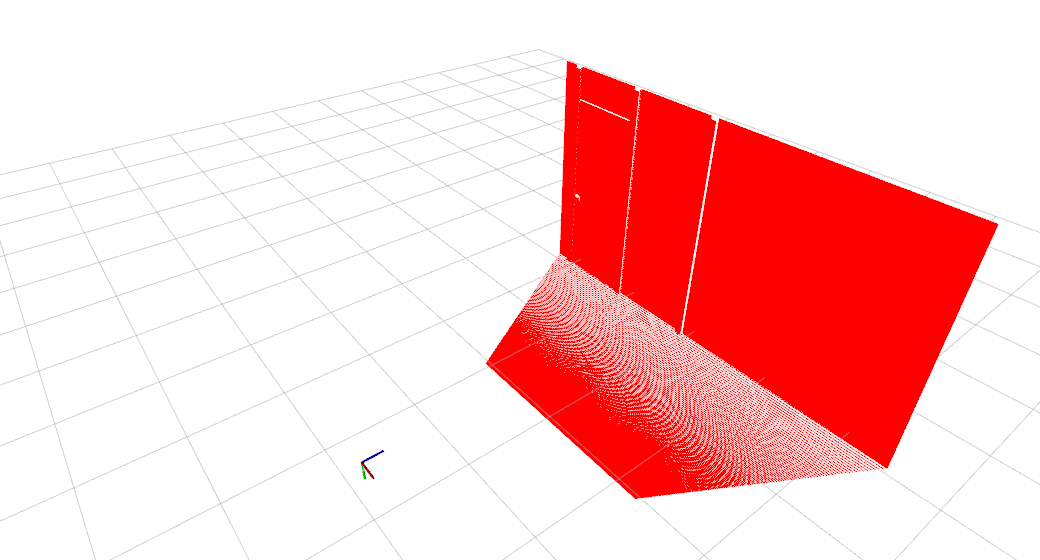
\includegraphics[width=0.5\linewidth]{images/pcl/Selection_060} &
  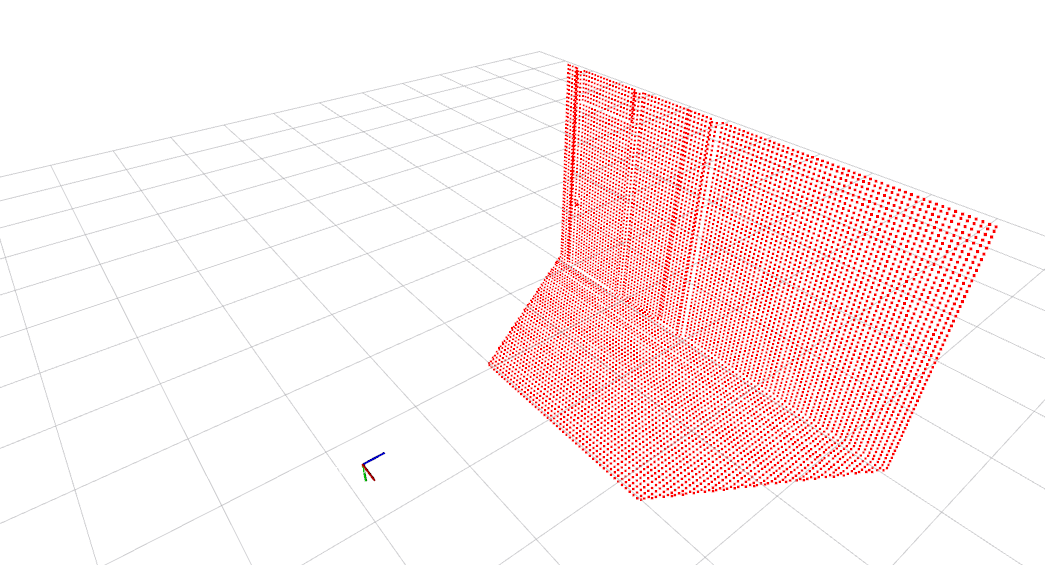
\includegraphics[width=0.5\linewidth]{images/pcl/Selection_061} \\
  (1) & (2) \\
  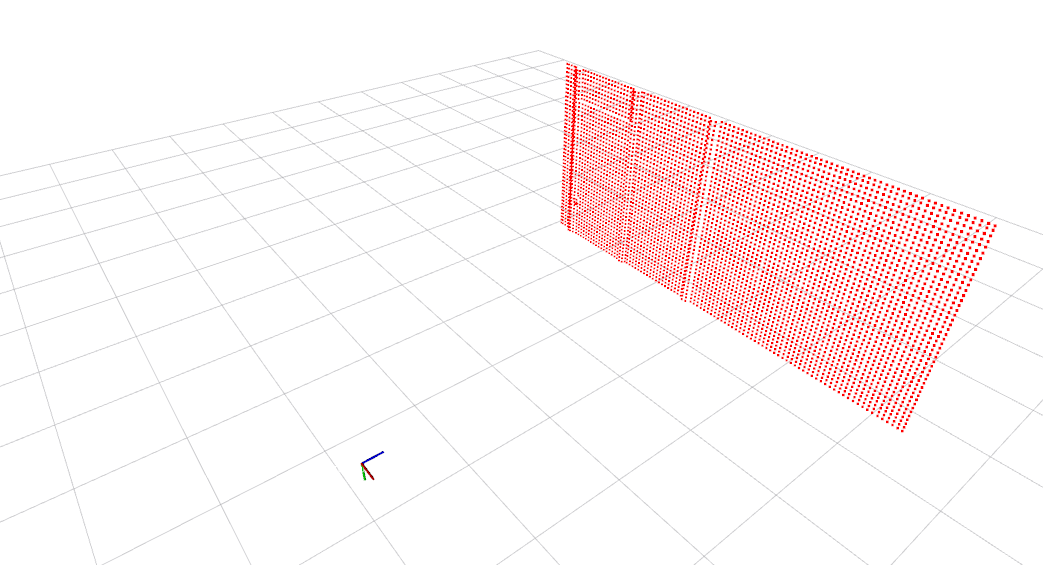
\includegraphics[width=0.5\linewidth]{images/pcl/Selection_062} &
  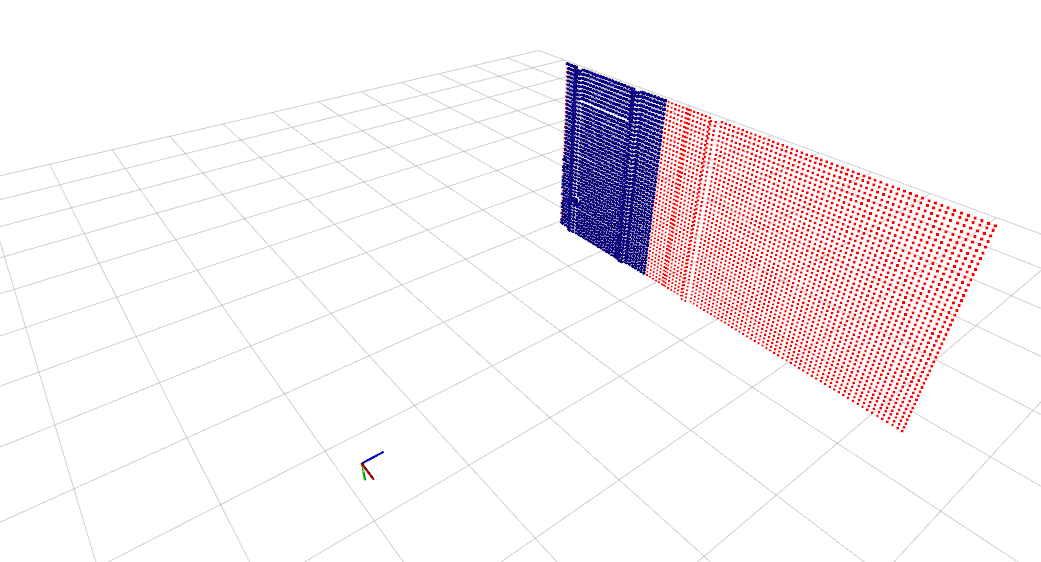
\includegraphics[width=0.5\linewidth]{images/pcl/Selection_063} \\
  (3) & (4) \\
  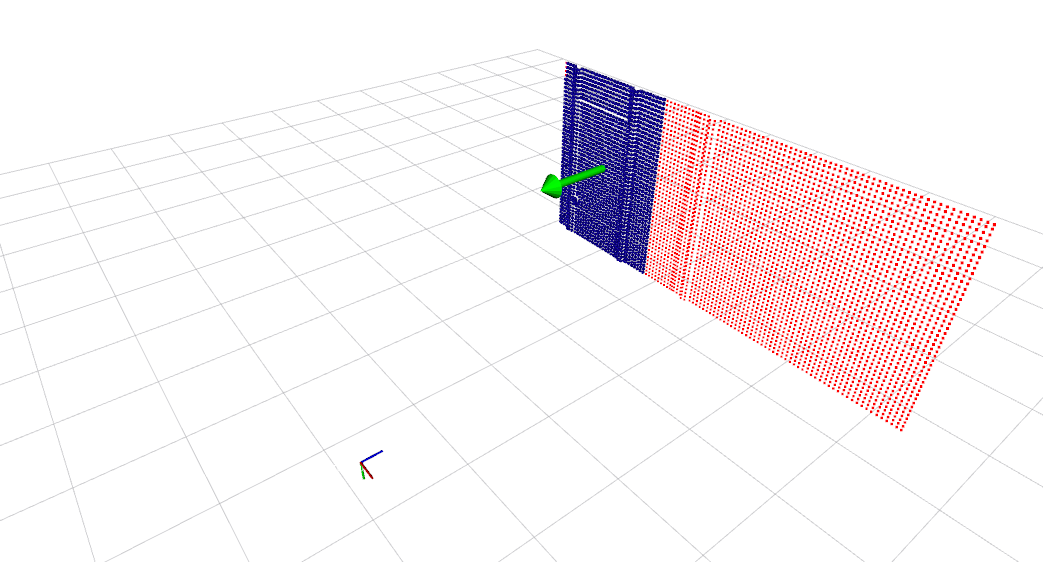
\includegraphics[width=0.5\linewidth]{images/pcl/Selection_064} &
  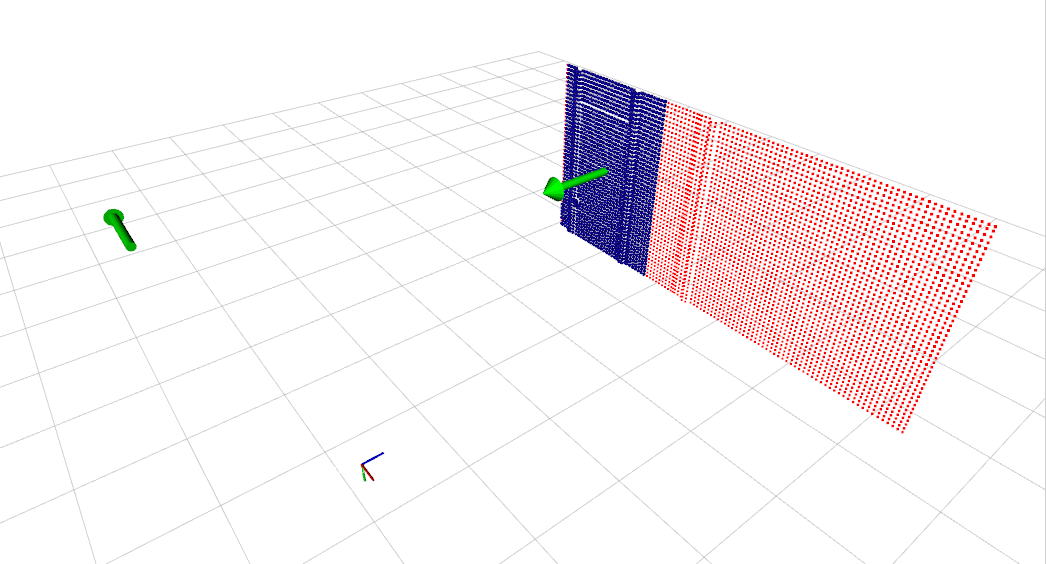
\includegraphics[width=0.5\linewidth]{images/pcl/Selection_065} \\
  (5) & (6)
\end{tabular}

(1) Nuage de points initial. (2) Downsampling du nuage. (3) Filtrage du sol par seuillage de la coordonnée $z$. (4) Sélection de un tiers du nuage vers l'avant du robot. (5) Calcul de la normale par ACP. (6) Calcul de la nouvelle pose objectif en prenant une longueur de pas dans la direction obtenue par le produit vectoriel entre la normale et l'axe $z$ du robot.

\Annexe{MACHINE À ÉTATS POUR L'INSPECTION D'ÉOLIENNES}
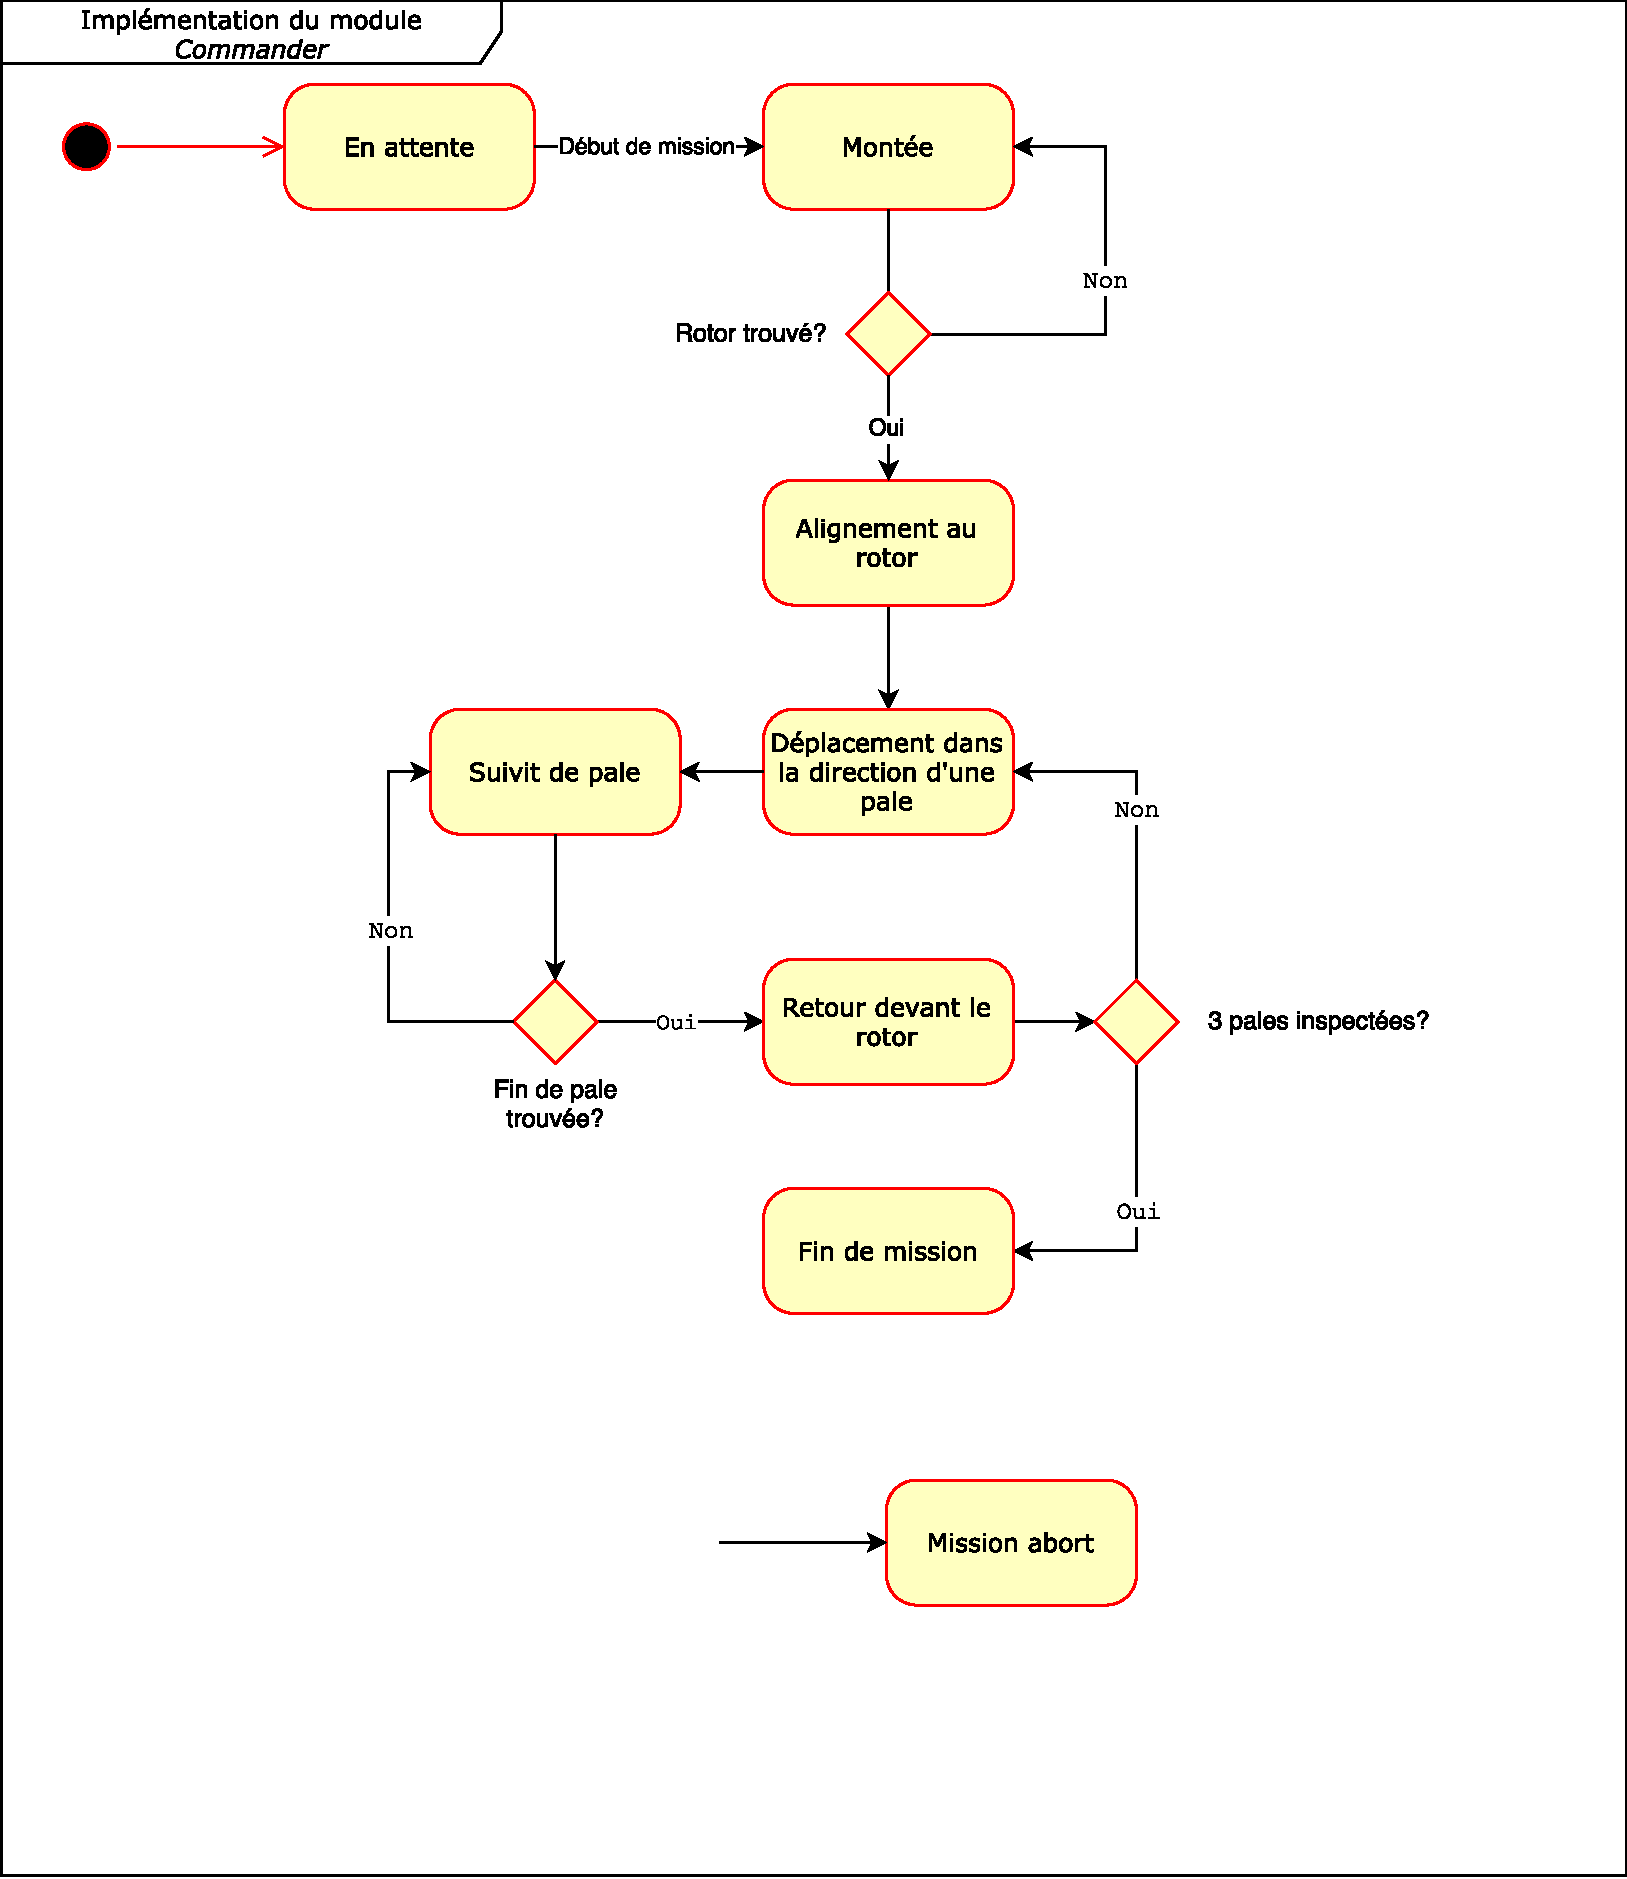
\includegraphics[width=\linewidth]{images/state_machine.pdf}
\label{annexe:state_machine}

\Annexe{LISTE DES PUBLICATIONS}
\begin{longtable}{lp{5in}}
  [Journal]     & A. Borowczyk, D.-T. Nguyen, \textbf{A. Phu-Van Nguyen}, D. Q. Nguyen, D. Saussié and J. Le Ny, \textit{Autonomous Landing of a Quadcopter on a High-Speed Ground Vehicle}. AIAA Journal of Guidance, Control and Dynamics, In Press, 2017.\\

  [Conférence]  & A. Borowczyk, D.-T. Nguyen, \textbf{A. Phu-Van Nguyen}, D. Q. Nguyen, D. Saussié and J. Le Ny, \textit{Autonomous Landing of a Multirotor Micro Air Vehicle on a High Velocity Ground Vehicle}. Proceedings of the IFAC World Congress, Toulouse, France, July 2017.\\

  [Journal]      & M. S. Ramanagopal, \textbf{A. Phu-Van Nguyen} and J. Le Ny, A Motion Planning Strategy for the Active Vision-Based Mapping of Ground-Level Structures. Accepted by Transactions on Automation Science and Engineering, November 2017.
\end{longtable}

Le travail des deux premières publications à propos de l'atterrissage d'un quadricoptère sur une voiture en mouvement a été réalisé dans le cadre de la participation du \textit{Mobile Robotics and Autonomous Systems Laboratory} au DJI Challenge lors des session d'hiver et d'été 2016. N'étant pas directement liées au présent mémoire, elles sont mentionnées ici car plusieurs des méthodes de contrôle de véhicule aérien et de traitement d'images ont été apprises lors de notre participation à cette compétition. Mon rôle spéficique dans ce projet était l'aide au traitement d'images pour la détection de la plateforme d'atterrissage et l'aide au niveau de l'implémentation du système en C++.

La dernière publication intitulée \textit{A Motion Planning Strategy for the Active Vision-Based Mapping of Ground-Level Structures} a été initialement soumise en février 2016 par M. S. Ramanagopal et J. Le Ny au journal \textit{Transactions on Automation Science and Engineering} (T-ASE). Lors du retour de l'évaluation par les pairs, il a été demandé entres autres d'ajouter un volet expérimental à l'article afin de prouver la validité des algorithmes développés dans l'article. C'est à ce moment, lors de la session d'automne 2016 et au début de la session d'hiver 2017 que je me suis ajouté au projet pour faire l'implémentation sur un robot physique. Au moment de l'écriture du présent mémoire, l'article a été accepté pour publication dans une édition future du journal T-ASE. Nous présentons le travail réalisé dans le cadre de ce projet au Chapitre \ref{sec:ugv}.


%%  Toutes les annexes doivent être inclues dans ce document
%%  les unes à la suite des autres.
% \Annexe{DÉMO}
% Texte de l'annexe A\@. Remarquez que la phrase précédente se termine
% par une lettre majuscule suivie d'un point. On indique explicitement
% cette situation à \LaTeX{} afin que ce dernier ajuste correctement
% l'espacement entre le point final de la phrase et le début de la
% phrase suivante.


%\begin{landscape}
%\Annexe{ENCORE UNE ANNEXE}
%Texte de l'annexe B\@ en mode «landscape».
%\end{landscape}
%
%\Annexe{UNE DERNIÈRE ANNEXE}
%Texte de l'annexe C\@.
}{}
\end{document}
